% Options for packages loaded elsewhere
\PassOptionsToPackage{unicode}{hyperref}
\PassOptionsToPackage{hyphens}{url}
%
\documentclass[
]{article}
\usepackage{amsmath,amssymb}
\usepackage{iftex}
\ifPDFTeX
  \usepackage[T1]{fontenc}
  \usepackage[utf8]{inputenc}
  \usepackage{textcomp} % provide euro and other symbols
\else % if luatex or xetex
  \usepackage{unicode-math} % this also loads fontspec
  \defaultfontfeatures{Scale=MatchLowercase}
  \defaultfontfeatures[\rmfamily]{Ligatures=TeX,Scale=1}
\fi
\usepackage{lmodern}
\ifPDFTeX\else
  % xetex/luatex font selection
\fi
% Use upquote if available, for straight quotes in verbatim environments
\IfFileExists{upquote.sty}{\usepackage{upquote}}{}
\IfFileExists{microtype.sty}{% use microtype if available
  \usepackage[]{microtype}
  \UseMicrotypeSet[protrusion]{basicmath} % disable protrusion for tt fonts
}{}
\makeatletter
\@ifundefined{KOMAClassName}{% if non-KOMA class
  \IfFileExists{parskip.sty}{%
    \usepackage{parskip}
  }{% else
    \setlength{\parindent}{0pt}
    \setlength{\parskip}{6pt plus 2pt minus 1pt}}
}{% if KOMA class
  \KOMAoptions{parskip=half}}
\makeatother
\usepackage{xcolor}
\usepackage[margin=1in]{geometry}
\usepackage{color}
\usepackage{fancyvrb}
\newcommand{\VerbBar}{|}
\newcommand{\VERB}{\Verb[commandchars=\\\{\}]}
\DefineVerbatimEnvironment{Highlighting}{Verbatim}{commandchars=\\\{\}}
% Add ',fontsize=\small' for more characters per line
\usepackage{framed}
\definecolor{shadecolor}{RGB}{248,248,248}
\newenvironment{Shaded}{\begin{snugshade}}{\end{snugshade}}
\newcommand{\AlertTok}[1]{\textcolor[rgb]{0.94,0.16,0.16}{#1}}
\newcommand{\AnnotationTok}[1]{\textcolor[rgb]{0.56,0.35,0.01}{\textbf{\textit{#1}}}}
\newcommand{\AttributeTok}[1]{\textcolor[rgb]{0.13,0.29,0.53}{#1}}
\newcommand{\BaseNTok}[1]{\textcolor[rgb]{0.00,0.00,0.81}{#1}}
\newcommand{\BuiltInTok}[1]{#1}
\newcommand{\CharTok}[1]{\textcolor[rgb]{0.31,0.60,0.02}{#1}}
\newcommand{\CommentTok}[1]{\textcolor[rgb]{0.56,0.35,0.01}{\textit{#1}}}
\newcommand{\CommentVarTok}[1]{\textcolor[rgb]{0.56,0.35,0.01}{\textbf{\textit{#1}}}}
\newcommand{\ConstantTok}[1]{\textcolor[rgb]{0.56,0.35,0.01}{#1}}
\newcommand{\ControlFlowTok}[1]{\textcolor[rgb]{0.13,0.29,0.53}{\textbf{#1}}}
\newcommand{\DataTypeTok}[1]{\textcolor[rgb]{0.13,0.29,0.53}{#1}}
\newcommand{\DecValTok}[1]{\textcolor[rgb]{0.00,0.00,0.81}{#1}}
\newcommand{\DocumentationTok}[1]{\textcolor[rgb]{0.56,0.35,0.01}{\textbf{\textit{#1}}}}
\newcommand{\ErrorTok}[1]{\textcolor[rgb]{0.64,0.00,0.00}{\textbf{#1}}}
\newcommand{\ExtensionTok}[1]{#1}
\newcommand{\FloatTok}[1]{\textcolor[rgb]{0.00,0.00,0.81}{#1}}
\newcommand{\FunctionTok}[1]{\textcolor[rgb]{0.13,0.29,0.53}{\textbf{#1}}}
\newcommand{\ImportTok}[1]{#1}
\newcommand{\InformationTok}[1]{\textcolor[rgb]{0.56,0.35,0.01}{\textbf{\textit{#1}}}}
\newcommand{\KeywordTok}[1]{\textcolor[rgb]{0.13,0.29,0.53}{\textbf{#1}}}
\newcommand{\NormalTok}[1]{#1}
\newcommand{\OperatorTok}[1]{\textcolor[rgb]{0.81,0.36,0.00}{\textbf{#1}}}
\newcommand{\OtherTok}[1]{\textcolor[rgb]{0.56,0.35,0.01}{#1}}
\newcommand{\PreprocessorTok}[1]{\textcolor[rgb]{0.56,0.35,0.01}{\textit{#1}}}
\newcommand{\RegionMarkerTok}[1]{#1}
\newcommand{\SpecialCharTok}[1]{\textcolor[rgb]{0.81,0.36,0.00}{\textbf{#1}}}
\newcommand{\SpecialStringTok}[1]{\textcolor[rgb]{0.31,0.60,0.02}{#1}}
\newcommand{\StringTok}[1]{\textcolor[rgb]{0.31,0.60,0.02}{#1}}
\newcommand{\VariableTok}[1]{\textcolor[rgb]{0.00,0.00,0.00}{#1}}
\newcommand{\VerbatimStringTok}[1]{\textcolor[rgb]{0.31,0.60,0.02}{#1}}
\newcommand{\WarningTok}[1]{\textcolor[rgb]{0.56,0.35,0.01}{\textbf{\textit{#1}}}}
\usepackage{longtable,booktabs,array}
\usepackage{calc} % for calculating minipage widths
% Correct order of tables after \paragraph or \subparagraph
\usepackage{etoolbox}
\makeatletter
\patchcmd\longtable{\par}{\if@noskipsec\mbox{}\fi\par}{}{}
\makeatother
% Allow footnotes in longtable head/foot
\IfFileExists{footnotehyper.sty}{\usepackage{footnotehyper}}{\usepackage{footnote}}
\makesavenoteenv{longtable}
\usepackage{graphicx}
\makeatletter
\def\maxwidth{\ifdim\Gin@nat@width>\linewidth\linewidth\else\Gin@nat@width\fi}
\def\maxheight{\ifdim\Gin@nat@height>\textheight\textheight\else\Gin@nat@height\fi}
\makeatother
% Scale images if necessary, so that they will not overflow the page
% margins by default, and it is still possible to overwrite the defaults
% using explicit options in \includegraphics[width, height, ...]{}
\setkeys{Gin}{width=\maxwidth,height=\maxheight,keepaspectratio}
% Set default figure placement to htbp
\makeatletter
\def\fps@figure{htbp}
\makeatother
\setlength{\emergencystretch}{3em} % prevent overfull lines
\providecommand{\tightlist}{%
  \setlength{\itemsep}{0pt}\setlength{\parskip}{0pt}}
\setcounter{secnumdepth}{5}
\usepackage{pdfpages}
\usepackage{tcolorbox}
\usepackage{graphicx}
\usepackage{setspace}
\usepackage{booktabs}
\usepackage{caption}
\usepackage{longtable}
\usepackage{multirow}
\usepackage{multicol}
\usepackage{colortbl}
\usepackage{hhline}
\newlength\Oldarrayrulewidth
\newlength\Oldtabcolsep
\usepackage{array}
\usepackage{hyperref}
\usepackage{float}
\usepackage{wrapfig}
\ifLuaTeX
  \usepackage{selnolig}  % disable illegal ligatures
\fi
\IfFileExists{bookmark.sty}{\usepackage{bookmark}}{\usepackage{hyperref}}
\IfFileExists{xurl.sty}{\usepackage{xurl}}{} % add URL line breaks if available
\urlstyle{same}
\hypersetup{
  hidelinks,
  pdfcreator={LaTeX via pandoc}}

\author{}
\date{\vspace{-2.5em}}

\begin{document}

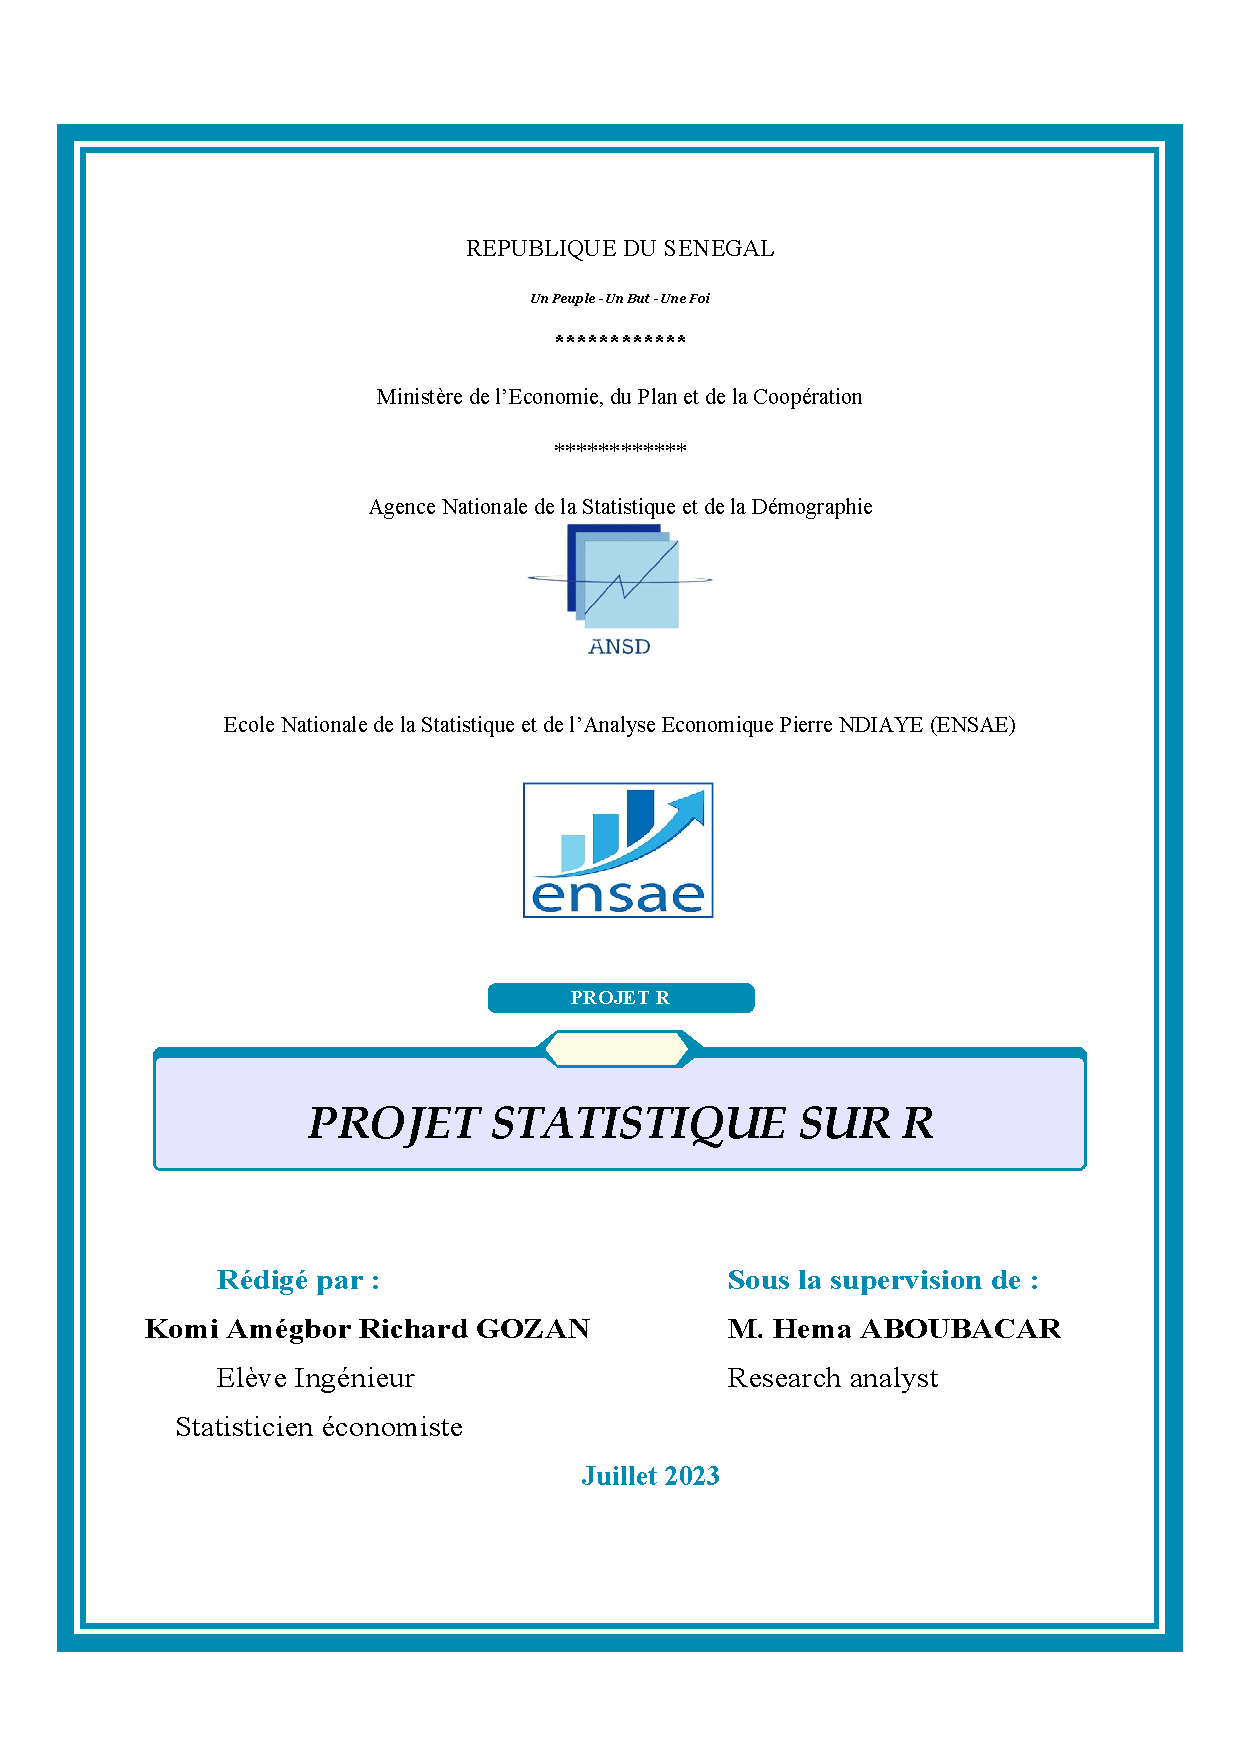
\includepdf{page}

\newpage

\setstretch{1.5}

\renewcommand{\contentsname}{\textcolor{blue}{Table des matières}}

\textcolor{blue}{\tableofcontents}

\newpage

\hypertarget{chargement-des-packages}{%
\section{Chargement des packages}\label{chargement-des-packages}}

\begin{Shaded}
\begin{Highlighting}[]
\FunctionTok{library}\NormalTok{(readxl)}
\FunctionTok{library}\NormalTok{(dplyr)}
\FunctionTok{library}\NormalTok{(gtsummary)}
\FunctionTok{library}\NormalTok{(gt)}
\FunctionTok{library}\NormalTok{(sf)}
\FunctionTok{library}\NormalTok{(leaflet)}
\FunctionTok{library}\NormalTok{(ggplot2)}
\FunctionTok{library}\NormalTok{(flextable)}
\FunctionTok{library}\NormalTok{(ggspatial)}
\FunctionTok{library}\NormalTok{(broom)}
\FunctionTok{library}\NormalTok{(questionr)}
\FunctionTok{library}\NormalTok{(lubridate)}
\FunctionTok{library}\NormalTok{(GGally)}
\end{Highlighting}
\end{Shaded}

\hypertarget{partie-1}{%
\section{Partie 1}\label{partie-1}}

\hypertarget{pruxe9paration-des-donnuxe9es}{%
\subsection{Préparation des
données}\label{pruxe9paration-des-donnuxe9es}}

\hypertarget{decription}{%
\subsubsection{Decription}\label{decription}}

\hypertarget{importation-et-mise-en-forme}{%
\subsubsection{Importation et mise en
forme}\label{importation-et-mise-en-forme}}

\begin{itemize}
\tightlist
\item
  Importation de la base de données dans un objet de type data.frame
  nommé projet :
\end{itemize}

\begin{Shaded}
\begin{Highlighting}[]
\NormalTok{projet }\OtherTok{\textless{}{-}} \FunctionTok{read\_excel}\NormalTok{(}\StringTok{"Bases/Base\_Partie 1.xlsx"}\NormalTok{)}
\end{Highlighting}
\end{Shaded}

\begin{itemize}
\tightlist
\item
  Tableau résumant les valeurs manquantes par variable :
\end{itemize}

\begin{Shaded}
\begin{Highlighting}[]
\NormalTok{df }\OtherTok{=} \FunctionTok{data.frame}\NormalTok{(}\AttributeTok{variables =} \FunctionTok{colnames}\NormalTok{(projet),}\AttributeTok{Valeurs\_manquantes =} \FunctionTok{colSums}\NormalTok{(}\FunctionTok{is.na}\NormalTok{(projet)))}
\NormalTok{df }\SpecialCharTok{\%\textgreater{}\%} \FunctionTok{gt}\NormalTok{()}
\end{Highlighting}
\end{Shaded}

\begin{longtable}{lr}
\toprule
variables & Valeurs\_manquantes \\ 
\midrule
key & 0 \\ 
q1 & 0 \\ 
q2 & 0 \\ 
q23 & 0 \\ 
q24 & 0 \\ 
q24a\_1 & 0 \\ 
q24a\_2 & 0 \\ 
q24a\_3 & 0 \\ 
q24a\_4 & 0 \\ 
q24a\_5 & 0 \\ 
q24a\_6 & 0 \\ 
q24a\_7 & 0 \\ 
q24a\_9 & 0 \\ 
q24a\_10 & 0 \\ 
q25 & 0 \\ 
q26 & 0 \\ 
q12 & 0 \\ 
q14b & 1 \\ 
q16 & 1 \\ 
q17 & 131 \\ 
q19 & 120 \\ 
q20 & 0 \\ 
filiere\_1 & 0 \\ 
filiere\_2 & 0 \\ 
filiere\_3 & 0 \\ 
filiere\_4 & 0 \\ 
q8 & 0 \\ 
q81 & 0 \\ 
gps\_menlatitude & 0 \\ 
gps\_menlongitude & 0 \\ 
submissiondate & 0 \\ 
start & 0 \\ 
today & 0 \\ 
\bottomrule
\end{longtable}

\begin{itemize}
\tightlist
\item
  Vérifions s'il y a des valeurs manquantes pour la variable key dans la
  base projet. Si oui, nous identifierons la (ou les) PME concernée(s).
\end{itemize}

\hypertarget{cruxe9ation-de-variables}{%
\subsubsection{Création de variables}\label{cruxe9ation-de-variables}}

\begin{itemize}
\tightlist
\item
  Renommage des variables
\end{itemize}

\begin{Shaded}
\begin{Highlighting}[]
\CommentTok{\# q1 en region, q2 en déparement et q23 en sexe}
\NormalTok{projet }\OtherTok{\textless{}{-}}\NormalTok{ projet }\SpecialCharTok{\%\textgreater{}\%}
  \FunctionTok{rename}\NormalTok{(}\AttributeTok{region =}\NormalTok{ q1, }\AttributeTok{departement =}\NormalTok{ q2, }\AttributeTok{sexe =}\NormalTok{ q23)}
\end{Highlighting}
\end{Shaded}

\begin{itemize}
\tightlist
\item
  Création de la variable sexe\_2 vallant 1 si sexe égale à Femme et 0
  sinon
\end{itemize}

\begin{Shaded}
\begin{Highlighting}[]
\NormalTok{projet }\OtherTok{\textless{}{-}}\NormalTok{ projet }\SpecialCharTok{\%\textgreater{}\%}
  \FunctionTok{mutate}\NormalTok{(}\AttributeTok{sexe\_2 =} \FunctionTok{ifelse}\NormalTok{(sexe }\SpecialCharTok{==} \StringTok{"Femme"}\NormalTok{, }\DecValTok{1}\NormalTok{, }\DecValTok{0}\NormalTok{))}
\end{Highlighting}
\end{Shaded}

\begin{itemize}
\tightlist
\item
  Création du data.frame ``langues''
\end{itemize}

\begin{Shaded}
\begin{Highlighting}[]
\NormalTok{langues }\OtherTok{\textless{}{-}}\NormalTok{ projet }\SpecialCharTok{\%\textgreater{}\%}
  \FunctionTok{select}\NormalTok{(key, }\FunctionTok{starts\_with}\NormalTok{(}\StringTok{"q24a\_"}\NormalTok{))}
\end{Highlighting}
\end{Shaded}

\begin{itemize}
\tightlist
\item
  Création de la variable ``parle''
\end{itemize}

\begin{Shaded}
\begin{Highlighting}[]
\NormalTok{langues }\OtherTok{\textless{}{-}}\NormalTok{ langues }\SpecialCharTok{\%\textgreater{}\%}
  \FunctionTok{mutate}\NormalTok{(}\AttributeTok{parle =} \FunctionTok{rowSums}\NormalTok{(.[}\DecValTok{2}\SpecialCharTok{:}\FunctionTok{ncol}\NormalTok{(.)]))}
\end{Highlighting}
\end{Shaded}

\begin{itemize}
\tightlist
\item
  Sélection des variables ``key'' et ``parle''
\end{itemize}

\begin{Shaded}
\begin{Highlighting}[]
\NormalTok{langues }\OtherTok{\textless{}{-}}\NormalTok{ langues }\SpecialCharTok{\%\textgreater{}\%}
  \FunctionTok{select}\NormalTok{(key, parle)}
\end{Highlighting}
\end{Shaded}

\begin{itemize}
\tightlist
\item
  Mergons les data.frame ``projet'' et ``langues''
\end{itemize}

\begin{Shaded}
\begin{Highlighting}[]
\NormalTok{projet }\OtherTok{\textless{}{-}}\NormalTok{ projet }\SpecialCharTok{\%\textgreater{}\%}
  \FunctionTok{left\_join}\NormalTok{(langues, }\AttributeTok{by =} \StringTok{"key"}\NormalTok{)}
\end{Highlighting}
\end{Shaded}

\hypertarget{statistiques-descriptives}{%
\subsection{Statistiques descriptives}\label{statistiques-descriptives}}

\hypertarget{satistiques-descriptives-demanduxe9es}{%
\subsubsection{Satistiques descriptives
demandées}\label{satistiques-descriptives-demanduxe9es}}

Il nous est demandé la répartion des PME suivant:

• le sexe

• le niveau d'instruction

• le statut juridique

• le propriétaire/locataire

• le statut juridique et le sexe

• le niveau d'instruction et le sexe

• Propriétaire/locataire suivant le sexe

Nous résumons ces répartitions dans un seul tableau avec l'analyse
univariée et l'anlyse buvariée

\begin{Shaded}
\begin{Highlighting}[]
\CommentTok{\# Répartition des PME suivant le sexe, le niveau d\textquotesingle{}instruction,}
\CommentTok{\# le statut juridique et le propriétaire locataire}
\NormalTok{tbl1 }\OtherTok{\textless{}{-}}\NormalTok{ projet }\SpecialCharTok{\%\textgreater{}\%} \FunctionTok{tbl\_summary}\NormalTok{(}
  \AttributeTok{include =} \FunctionTok{c}\NormalTok{(}\StringTok{"sexe"}\NormalTok{, }\StringTok{"q25"}\NormalTok{, }\StringTok{"q12"}\NormalTok{, }\StringTok{"q81"}\NormalTok{),}
  \AttributeTok{label=}\FunctionTok{list}\NormalTok{(q25}\SpecialCharTok{\textasciitilde{}} \StringTok{"Niveau d\textquotesingle{}instruction"}\NormalTok{, }
\NormalTok{             q12}\SpecialCharTok{\textasciitilde{}} \StringTok{"Statut juridique"}\NormalTok{,}
\NormalTok{             q81}\SpecialCharTok{\textasciitilde{}} \StringTok{"Propriétaire/locataire"}\NormalTok{))}

\CommentTok{\# Répartition des PME suivant le statut juridique et le sexe,}
\CommentTok{\# le niveau d’instruction et le sexe,   Propriétaire/locataire}
\CommentTok{\# et le sexe}
\NormalTok{tbl2 }\OtherTok{\textless{}{-}}\NormalTok{ projet }\SpecialCharTok{\%\textgreater{}\%} \FunctionTok{tbl\_summary}\NormalTok{(}
  \AttributeTok{include =} \FunctionTok{c}\NormalTok{(}\StringTok{"q25"}\NormalTok{, }\StringTok{"q12"}\NormalTok{, }\StringTok{"q81"}\NormalTok{), }
  \AttributeTok{by =}\StringTok{"sexe"}\NormalTok{, }\AttributeTok{label=}\FunctionTok{list}\NormalTok{(q12}\SpecialCharTok{\textasciitilde{}} \StringTok{"Statut juridique"}\NormalTok{, }
\NormalTok{                         q25}\SpecialCharTok{\textasciitilde{}} \StringTok{"Niveau d\textquotesingle{}instruction"}\NormalTok{, }
\NormalTok{                         q81}\SpecialCharTok{\textasciitilde{}} \StringTok{"Propriétaire/locataire"}\NormalTok{)) }\SpecialCharTok{\%\textgreater{}\%} 
  \FunctionTok{modify\_header}\NormalTok{(label }\SpecialCharTok{\textasciitilde{}} \StringTok{"**Variables**"}\NormalTok{) }\SpecialCharTok{\%\textgreater{}\%}
  \FunctionTok{modify\_spanning\_header}\NormalTok{(}\FunctionTok{all\_stat\_cols}\NormalTok{() }\SpecialCharTok{\textasciitilde{}} \StringTok{"**Sexe**"}\NormalTok{) }\SpecialCharTok{\%\textgreater{}\%}
  \FunctionTok{bold\_labels}\NormalTok{()}

\DocumentationTok{\#\# Empillement l\textquotesingle{}une sur l\textquotesingle{}autre}
\FunctionTok{tbl\_merge}\NormalTok{(}
    \AttributeTok{tbls =} \FunctionTok{list}\NormalTok{(tbl1, tbl2),}
    \AttributeTok{tab\_spanner =} \FunctionTok{c}\NormalTok{(}\StringTok{"**Analyse univariée**"}\NormalTok{, }\StringTok{"**Analye bivariée**"}\NormalTok{)) }\SpecialCharTok{\%\textgreater{}\%}
  \FunctionTok{italicize\_levels}\NormalTok{() }\SpecialCharTok{\%\textgreater{}\%}
  \FunctionTok{as\_flex\_table}\NormalTok{() }\SpecialCharTok{\%\textgreater{}\%}
  \FunctionTok{fontsize}\NormalTok{(}\AttributeTok{size=}\DecValTok{10}\NormalTok{) }\SpecialCharTok{\%\textgreater{}\%}
  \FunctionTok{width}\NormalTok{(}\AttributeTok{width =} \FloatTok{1.3}\NormalTok{)}
\end{Highlighting}
\end{Shaded}

\global\setlength{\Oldarrayrulewidth}{\arrayrulewidth}

\global\setlength{\Oldtabcolsep}{\tabcolsep}

\setlength{\tabcolsep}{0pt}

\renewcommand*{\arraystretch}{1.5}



\providecommand{\ascline}[3]{\noalign{\global\arrayrulewidth #1}\arrayrulecolor[HTML]{#2}\cline{#3}}

\begin{longtable}[c]{|p{1.30in}|p{1.30in}|p{1.30in}|p{1.30in}}



\ascline{1pt}{000000}{1-4}

\multicolumn{1}{>{\raggedright}m{\dimexpr 1.3in+0\tabcolsep}}{\textcolor[HTML]{000000}{\fontsize{11}{11}\selectfont{\ }}} & \multicolumn{1}{>{\centering}m{\dimexpr 1.3in+0\tabcolsep}}{\textcolor[HTML]{000000}{\fontsize{11}{11}\selectfont{\textbf{Analyse\ univariée}}}} & \multicolumn{2}{>{\centering}m{\dimexpr 2.6in+2\tabcolsep}}{\textcolor[HTML]{000000}{\fontsize{11}{11}\selectfont{\textbf{Analye\ bivariée}}}} \\

\ascline{1pt}{000000}{1-4}



\multicolumn{1}{>{\raggedright}m{\dimexpr 1.3in+0\tabcolsep}}{\textcolor[HTML]{000000}{\fontsize{11}{11}\selectfont{\textbf{Characteristic}}}} & \multicolumn{1}{>{\centering}m{\dimexpr 1.3in+0\tabcolsep}}{\textcolor[HTML]{000000}{\fontsize{11}{11}\selectfont{\textbf{N\ =\ 250}}}\textcolor[HTML]{000000}{\textsuperscript{\fontsize{11}{11}\selectfont{1}}}} & \multicolumn{1}{>{\centering}m{\dimexpr 1.3in+0\tabcolsep}}{\textcolor[HTML]{000000}{\fontsize{11}{11}\selectfont{\textbf{Femme}}}\textcolor[HTML]{000000}{\fontsize{11}{11}\selectfont{,\ N\ =\ 191}}\textcolor[HTML]{000000}{\textsuperscript{\fontsize{11}{11}\selectfont{1}}}} & \multicolumn{1}{>{\centering}m{\dimexpr 1.3in+0\tabcolsep}}{\textcolor[HTML]{000000}{\fontsize{11}{11}\selectfont{\textbf{Homme}}}\textcolor[HTML]{000000}{\fontsize{11}{11}\selectfont{,\ N\ =\ 59}}\textcolor[HTML]{000000}{\textsuperscript{\fontsize{11}{11}\selectfont{1}}}} \\

\ascline{1pt}{000000}{1-4}\endfirsthead 

\ascline{1pt}{000000}{1-4}

\multicolumn{1}{>{\raggedright}m{\dimexpr 1.3in+0\tabcolsep}}{\textcolor[HTML]{000000}{\fontsize{11}{11}\selectfont{\ }}} & \multicolumn{1}{>{\centering}m{\dimexpr 1.3in+0\tabcolsep}}{\textcolor[HTML]{000000}{\fontsize{11}{11}\selectfont{\textbf{Analyse\ univariée}}}} & \multicolumn{2}{>{\centering}m{\dimexpr 2.6in+2\tabcolsep}}{\textcolor[HTML]{000000}{\fontsize{11}{11}\selectfont{\textbf{Analye\ bivariée}}}} \\

\ascline{1pt}{000000}{1-4}



\multicolumn{1}{>{\raggedright}m{\dimexpr 1.3in+0\tabcolsep}}{\textcolor[HTML]{000000}{\fontsize{11}{11}\selectfont{\textbf{Characteristic}}}} & \multicolumn{1}{>{\centering}m{\dimexpr 1.3in+0\tabcolsep}}{\textcolor[HTML]{000000}{\fontsize{11}{11}\selectfont{\textbf{N\ =\ 250}}}\textcolor[HTML]{000000}{\textsuperscript{\fontsize{11}{11}\selectfont{1}}}} & \multicolumn{1}{>{\centering}m{\dimexpr 1.3in+0\tabcolsep}}{\textcolor[HTML]{000000}{\fontsize{11}{11}\selectfont{\textbf{Femme}}}\textcolor[HTML]{000000}{\fontsize{11}{11}\selectfont{,\ N\ =\ 191}}\textcolor[HTML]{000000}{\textsuperscript{\fontsize{11}{11}\selectfont{1}}}} & \multicolumn{1}{>{\centering}m{\dimexpr 1.3in+0\tabcolsep}}{\textcolor[HTML]{000000}{\fontsize{11}{11}\selectfont{\textbf{Homme}}}\textcolor[HTML]{000000}{\fontsize{11}{11}\selectfont{,\ N\ =\ 59}}\textcolor[HTML]{000000}{\textsuperscript{\fontsize{11}{11}\selectfont{1}}}} \\

\ascline{1pt}{000000}{1-4}\endhead



\multicolumn{4}{>{\raggedright}m{\dimexpr 5.2in+6\tabcolsep}}{\textcolor[HTML]{000000}{\textsuperscript{\fontsize{11}{11}\selectfont{1}}}\textcolor[HTML]{000000}{\fontsize{11}{11}\selectfont{n\ (\%)}}} \\

\endfoot



\multicolumn{1}{>{\raggedright}p{\dimexpr 1.3in+0\tabcolsep}}{\textcolor[HTML]{000000}{\fontsize{10}{10}\selectfont{\textbf{sexe}}}} & \multicolumn{1}{>{\centering}p{\dimexpr 1.3in+0\tabcolsep}}{\textcolor[HTML]{000000}{\fontsize{10}{10}\selectfont{}}} & \multicolumn{1}{>{\centering}p{\dimexpr 1.3in+0\tabcolsep}}{\textcolor[HTML]{000000}{\fontsize{10}{10}\selectfont{}}} & \multicolumn{1}{>{\centering}p{\dimexpr 1.3in+0\tabcolsep}}{\textcolor[HTML]{000000}{\fontsize{10}{10}\selectfont{}}} \\





\multicolumn{1}{>{\raggedright}p{\dimexpr 1.3in+0\tabcolsep}}{\textcolor[HTML]{000000}{\fontsize{10}{10}\selectfont{\textit{Femme}}}} & \multicolumn{1}{>{\centering}p{\dimexpr 1.3in+0\tabcolsep}}{\textcolor[HTML]{000000}{\fontsize{10}{10}\selectfont{191\ (76\%)}}} & \multicolumn{1}{>{\centering}p{\dimexpr 1.3in+0\tabcolsep}}{\textcolor[HTML]{000000}{\fontsize{10}{10}\selectfont{}}} & \multicolumn{1}{>{\centering}p{\dimexpr 1.3in+0\tabcolsep}}{\textcolor[HTML]{000000}{\fontsize{10}{10}\selectfont{}}} \\





\multicolumn{1}{>{\raggedright}p{\dimexpr 1.3in+0\tabcolsep}}{\textcolor[HTML]{000000}{\fontsize{10}{10}\selectfont{\textit{Homme}}}} & \multicolumn{1}{>{\centering}p{\dimexpr 1.3in+0\tabcolsep}}{\textcolor[HTML]{000000}{\fontsize{10}{10}\selectfont{59\ (24\%)}}} & \multicolumn{1}{>{\centering}p{\dimexpr 1.3in+0\tabcolsep}}{\textcolor[HTML]{000000}{\fontsize{10}{10}\selectfont{}}} & \multicolumn{1}{>{\centering}p{\dimexpr 1.3in+0\tabcolsep}}{\textcolor[HTML]{000000}{\fontsize{10}{10}\selectfont{}}} \\





\multicolumn{1}{>{\raggedright}p{\dimexpr 1.3in+0\tabcolsep}}{\textcolor[HTML]{000000}{\fontsize{10}{10}\selectfont{\textbf{Niveau\ d'instruction}}}} & \multicolumn{1}{>{\centering}p{\dimexpr 1.3in+0\tabcolsep}}{\textcolor[HTML]{000000}{\fontsize{10}{10}\selectfont{}}} & \multicolumn{1}{>{\centering}p{\dimexpr 1.3in+0\tabcolsep}}{\textcolor[HTML]{000000}{\fontsize{10}{10}\selectfont{}}} & \multicolumn{1}{>{\centering}p{\dimexpr 1.3in+0\tabcolsep}}{\textcolor[HTML]{000000}{\fontsize{10}{10}\selectfont{}}} \\





\multicolumn{1}{>{\raggedright}p{\dimexpr 1.3in+0\tabcolsep}}{\textcolor[HTML]{000000}{\fontsize{10}{10}\selectfont{\textit{Aucun\ niveau}}}} & \multicolumn{1}{>{\centering}p{\dimexpr 1.3in+0\tabcolsep}}{\textcolor[HTML]{000000}{\fontsize{10}{10}\selectfont{79\ (32\%)}}} & \multicolumn{1}{>{\centering}p{\dimexpr 1.3in+0\tabcolsep}}{\textcolor[HTML]{000000}{\fontsize{10}{10}\selectfont{70\ (37\%)}}} & \multicolumn{1}{>{\centering}p{\dimexpr 1.3in+0\tabcolsep}}{\textcolor[HTML]{000000}{\fontsize{10}{10}\selectfont{9\ (15\%)}}} \\





\multicolumn{1}{>{\raggedright}p{\dimexpr 1.3in+0\tabcolsep}}{\textcolor[HTML]{000000}{\fontsize{10}{10}\selectfont{\textit{Niveau\ primaire}}}} & \multicolumn{1}{>{\centering}p{\dimexpr 1.3in+0\tabcolsep}}{\textcolor[HTML]{000000}{\fontsize{10}{10}\selectfont{56\ (22\%)}}} & \multicolumn{1}{>{\centering}p{\dimexpr 1.3in+0\tabcolsep}}{\textcolor[HTML]{000000}{\fontsize{10}{10}\selectfont{48\ (25\%)}}} & \multicolumn{1}{>{\centering}p{\dimexpr 1.3in+0\tabcolsep}}{\textcolor[HTML]{000000}{\fontsize{10}{10}\selectfont{8\ (14\%)}}} \\





\multicolumn{1}{>{\raggedright}p{\dimexpr 1.3in+0\tabcolsep}}{\textcolor[HTML]{000000}{\fontsize{10}{10}\selectfont{\textit{Niveau\ secondaire}}}} & \multicolumn{1}{>{\centering}p{\dimexpr 1.3in+0\tabcolsep}}{\textcolor[HTML]{000000}{\fontsize{10}{10}\selectfont{74\ (30\%)}}} & \multicolumn{1}{>{\centering}p{\dimexpr 1.3in+0\tabcolsep}}{\textcolor[HTML]{000000}{\fontsize{10}{10}\selectfont{56\ (29\%)}}} & \multicolumn{1}{>{\centering}p{\dimexpr 1.3in+0\tabcolsep}}{\textcolor[HTML]{000000}{\fontsize{10}{10}\selectfont{18\ (31\%)}}} \\





\multicolumn{1}{>{\raggedright}p{\dimexpr 1.3in+0\tabcolsep}}{\textcolor[HTML]{000000}{\fontsize{10}{10}\selectfont{\textit{Niveau\ Superieur}}}} & \multicolumn{1}{>{\centering}p{\dimexpr 1.3in+0\tabcolsep}}{\textcolor[HTML]{000000}{\fontsize{10}{10}\selectfont{41\ (16\%)}}} & \multicolumn{1}{>{\centering}p{\dimexpr 1.3in+0\tabcolsep}}{\textcolor[HTML]{000000}{\fontsize{10}{10}\selectfont{17\ (8.9\%)}}} & \multicolumn{1}{>{\centering}p{\dimexpr 1.3in+0\tabcolsep}}{\textcolor[HTML]{000000}{\fontsize{10}{10}\selectfont{24\ (41\%)}}} \\





\multicolumn{1}{>{\raggedright}p{\dimexpr 1.3in+0\tabcolsep}}{\textcolor[HTML]{000000}{\fontsize{10}{10}\selectfont{\textbf{Statut\ juridique}}}} & \multicolumn{1}{>{\centering}p{\dimexpr 1.3in+0\tabcolsep}}{\textcolor[HTML]{000000}{\fontsize{10}{10}\selectfont{}}} & \multicolumn{1}{>{\centering}p{\dimexpr 1.3in+0\tabcolsep}}{\textcolor[HTML]{000000}{\fontsize{10}{10}\selectfont{}}} & \multicolumn{1}{>{\centering}p{\dimexpr 1.3in+0\tabcolsep}}{\textcolor[HTML]{000000}{\fontsize{10}{10}\selectfont{}}} \\





\multicolumn{1}{>{\raggedright}p{\dimexpr 1.3in+0\tabcolsep}}{\textcolor[HTML]{000000}{\fontsize{10}{10}\selectfont{\textit{Association}}}} & \multicolumn{1}{>{\centering}p{\dimexpr 1.3in+0\tabcolsep}}{\textcolor[HTML]{000000}{\fontsize{10}{10}\selectfont{6\ (2.4\%)}}} & \multicolumn{1}{>{\centering}p{\dimexpr 1.3in+0\tabcolsep}}{\textcolor[HTML]{000000}{\fontsize{10}{10}\selectfont{3\ (1.6\%)}}} & \multicolumn{1}{>{\centering}p{\dimexpr 1.3in+0\tabcolsep}}{\textcolor[HTML]{000000}{\fontsize{10}{10}\selectfont{3\ (5.1\%)}}} \\





\multicolumn{1}{>{\raggedright}p{\dimexpr 1.3in+0\tabcolsep}}{\textcolor[HTML]{000000}{\fontsize{10}{10}\selectfont{\textit{GIE}}}} & \multicolumn{1}{>{\centering}p{\dimexpr 1.3in+0\tabcolsep}}{\textcolor[HTML]{000000}{\fontsize{10}{10}\selectfont{179\ (72\%)}}} & \multicolumn{1}{>{\centering}p{\dimexpr 1.3in+0\tabcolsep}}{\textcolor[HTML]{000000}{\fontsize{10}{10}\selectfont{149\ (78\%)}}} & \multicolumn{1}{>{\centering}p{\dimexpr 1.3in+0\tabcolsep}}{\textcolor[HTML]{000000}{\fontsize{10}{10}\selectfont{30\ (51\%)}}} \\





\multicolumn{1}{>{\raggedright}p{\dimexpr 1.3in+0\tabcolsep}}{\textcolor[HTML]{000000}{\fontsize{10}{10}\selectfont{\textit{Informel}}}} & \multicolumn{1}{>{\centering}p{\dimexpr 1.3in+0\tabcolsep}}{\textcolor[HTML]{000000}{\fontsize{10}{10}\selectfont{38\ (15\%)}}} & \multicolumn{1}{>{\centering}p{\dimexpr 1.3in+0\tabcolsep}}{\textcolor[HTML]{000000}{\fontsize{10}{10}\selectfont{32\ (17\%)}}} & \multicolumn{1}{>{\centering}p{\dimexpr 1.3in+0\tabcolsep}}{\textcolor[HTML]{000000}{\fontsize{10}{10}\selectfont{6\ (10\%)}}} \\





\multicolumn{1}{>{\raggedright}p{\dimexpr 1.3in+0\tabcolsep}}{\textcolor[HTML]{000000}{\fontsize{10}{10}\selectfont{\textit{SA}}}} & \multicolumn{1}{>{\centering}p{\dimexpr 1.3in+0\tabcolsep}}{\textcolor[HTML]{000000}{\fontsize{10}{10}\selectfont{7\ (2.8\%)}}} & \multicolumn{1}{>{\centering}p{\dimexpr 1.3in+0\tabcolsep}}{\textcolor[HTML]{000000}{\fontsize{10}{10}\selectfont{1\ (0.5\%)}}} & \multicolumn{1}{>{\centering}p{\dimexpr 1.3in+0\tabcolsep}}{\textcolor[HTML]{000000}{\fontsize{10}{10}\selectfont{6\ (10\%)}}} \\





\multicolumn{1}{>{\raggedright}p{\dimexpr 1.3in+0\tabcolsep}}{\textcolor[HTML]{000000}{\fontsize{10}{10}\selectfont{\textit{SARL}}}} & \multicolumn{1}{>{\centering}p{\dimexpr 1.3in+0\tabcolsep}}{\textcolor[HTML]{000000}{\fontsize{10}{10}\selectfont{13\ (5.2\%)}}} & \multicolumn{1}{>{\centering}p{\dimexpr 1.3in+0\tabcolsep}}{\textcolor[HTML]{000000}{\fontsize{10}{10}\selectfont{2\ (1.0\%)}}} & \multicolumn{1}{>{\centering}p{\dimexpr 1.3in+0\tabcolsep}}{\textcolor[HTML]{000000}{\fontsize{10}{10}\selectfont{11\ (19\%)}}} \\





\multicolumn{1}{>{\raggedright}p{\dimexpr 1.3in+0\tabcolsep}}{\textcolor[HTML]{000000}{\fontsize{10}{10}\selectfont{\textit{SUARL}}}} & \multicolumn{1}{>{\centering}p{\dimexpr 1.3in+0\tabcolsep}}{\textcolor[HTML]{000000}{\fontsize{10}{10}\selectfont{7\ (2.8\%)}}} & \multicolumn{1}{>{\centering}p{\dimexpr 1.3in+0\tabcolsep}}{\textcolor[HTML]{000000}{\fontsize{10}{10}\selectfont{4\ (2.1\%)}}} & \multicolumn{1}{>{\centering}p{\dimexpr 1.3in+0\tabcolsep}}{\textcolor[HTML]{000000}{\fontsize{10}{10}\selectfont{3\ (5.1\%)}}} \\





\multicolumn{1}{>{\raggedright}p{\dimexpr 1.3in+0\tabcolsep}}{\textcolor[HTML]{000000}{\fontsize{10}{10}\selectfont{\textbf{Propriétaire/locataire}}}} & \multicolumn{1}{>{\centering}p{\dimexpr 1.3in+0\tabcolsep}}{\textcolor[HTML]{000000}{\fontsize{10}{10}\selectfont{}}} & \multicolumn{1}{>{\centering}p{\dimexpr 1.3in+0\tabcolsep}}{\textcolor[HTML]{000000}{\fontsize{10}{10}\selectfont{}}} & \multicolumn{1}{>{\centering}p{\dimexpr 1.3in+0\tabcolsep}}{\textcolor[HTML]{000000}{\fontsize{10}{10}\selectfont{}}} \\





\multicolumn{1}{>{\raggedright}p{\dimexpr 1.3in+0\tabcolsep}}{\textcolor[HTML]{000000}{\fontsize{10}{10}\selectfont{\textit{Locataire}}}} & \multicolumn{1}{>{\centering}p{\dimexpr 1.3in+0\tabcolsep}}{\textcolor[HTML]{000000}{\fontsize{10}{10}\selectfont{24\ (9.6\%)}}} & \multicolumn{1}{>{\centering}p{\dimexpr 1.3in+0\tabcolsep}}{\textcolor[HTML]{000000}{\fontsize{10}{10}\selectfont{16\ (8.4\%)}}} & \multicolumn{1}{>{\centering}p{\dimexpr 1.3in+0\tabcolsep}}{\textcolor[HTML]{000000}{\fontsize{10}{10}\selectfont{8\ (14\%)}}} \\





\multicolumn{1}{>{\raggedright}p{\dimexpr 1.3in+0\tabcolsep}}{\textcolor[HTML]{000000}{\fontsize{10}{10}\selectfont{\textit{Propriétaire}}}} & \multicolumn{1}{>{\centering}p{\dimexpr 1.3in+0\tabcolsep}}{\textcolor[HTML]{000000}{\fontsize{10}{10}\selectfont{226\ (90\%)}}} & \multicolumn{1}{>{\centering}p{\dimexpr 1.3in+0\tabcolsep}}{\textcolor[HTML]{000000}{\fontsize{10}{10}\selectfont{175\ (92\%)}}} & \multicolumn{1}{>{\centering}p{\dimexpr 1.3in+0\tabcolsep}}{\textcolor[HTML]{000000}{\fontsize{10}{10}\selectfont{51\ (86\%)}}} \\

\ascline{1pt}{000000}{1-4}



\end{longtable}



\arrayrulecolor[HTML]{000000}

\global\setlength{\arrayrulewidth}{\Oldarrayrulewidth}

\global\setlength{\tabcolsep}{\Oldtabcolsep}

\renewcommand*{\arraystretch}{1}

\hypertarget{statistiques-descriptives-de-notre-choix-sur-les-autres-variables}{%
\subsubsection{Statistiques descriptives de notre choix sur les autres
variables:}\label{statistiques-descriptives-de-notre-choix-sur-les-autres-variables}}

\hypertarget{analyse-univariuxe9e}{%
\paragraph{Analyse univariée:}\label{analyse-univariuxe9e}}

\begin{itemize}
\tightlist
\item
  \textbf{Analyse des filières}
\end{itemize}

\begin{Shaded}
\begin{Highlighting}[]
\NormalTok{projet2 }\OtherTok{\textless{}{-}}\NormalTok{ projet }\SpecialCharTok{\%\textgreater{}\%}
  \FunctionTok{rename}\NormalTok{(}\AttributeTok{arachide =}\NormalTok{ filiere\_1, }\AttributeTok{anacarde =}\NormalTok{ filiere\_2, }\AttributeTok{mangue =}\NormalTok{ filiere\_3, }\AttributeTok{riz =}\NormalTok{filiere\_4)}
\NormalTok{projet2 }\SpecialCharTok{\%\textgreater{}\%} \FunctionTok{tbl\_summary}\NormalTok{(}
      \AttributeTok{include =} \FunctionTok{c}\NormalTok{(}\StringTok{"arachide"}\NormalTok{, }\StringTok{"anacarde"}\NormalTok{, }\StringTok{"mangue"}\NormalTok{, }\StringTok{"riz"}\NormalTok{),}
      \AttributeTok{label=}\FunctionTok{list}\NormalTok{(arachide}\SpecialCharTok{\textasciitilde{}} \StringTok{"Arachide"}\NormalTok{, }
\NormalTok{             anacarde}\SpecialCharTok{\textasciitilde{}} \StringTok{"anacarde"}\NormalTok{,}
\NormalTok{             mangue}\SpecialCharTok{\textasciitilde{}} \StringTok{"mangue"}\NormalTok{,}
\NormalTok{             riz}\SpecialCharTok{\textasciitilde{}} \StringTok{"riz"}\NormalTok{)) }\SpecialCharTok{\%\textgreater{}\%}
      \FunctionTok{bold\_labels}\NormalTok{()}
\end{Highlighting}
\end{Shaded}

\begin{longtable}[]{@{}lc@{}}
\toprule\noalign{}
\textbf{Characteristic} & \textbf{N = 250} \\
\midrule\noalign{}
\endhead
\bottomrule\noalign{}
\endlastfoot
\textbf{Arachide} & 108 (43\%) \\
\textbf{anacarde} & 61 (24\%) \\
\textbf{mangue} & 89 (36\%) \\
\textbf{riz} & 92 (37\%) \\
\end{longtable}

\begin{itemize}
\tightlist
\item
  \textbf{Statistiques descriptives pour les variables de date}
\end{itemize}

\begin{Shaded}
\begin{Highlighting}[]
\CommentTok{\# Nous copie notre objet projet dans l\textquotesingle{}objet data}
\NormalTok{data }\OtherTok{=}\NormalTok{ projet}
\CommentTok{\# Convertir les colonnes en format de date}
\NormalTok{data}\SpecialCharTok{$}\NormalTok{submissiondate }\OtherTok{\textless{}{-}} \FunctionTok{as\_date}\NormalTok{(data}\SpecialCharTok{$}\NormalTok{submissiondate)}
\NormalTok{data}\SpecialCharTok{$}\NormalTok{start }\OtherTok{\textless{}{-}} \FunctionTok{as\_date}\NormalTok{(data}\SpecialCharTok{$}\NormalTok{start)}
\NormalTok{data}\SpecialCharTok{$}\NormalTok{today }\OtherTok{\textless{}{-}} \FunctionTok{as\_date}\NormalTok{(data}\SpecialCharTok{$}\NormalTok{today)}

\CommentTok{\# Résumé statistique des colonnes de date}
\FunctionTok{summary}\NormalTok{(data}\SpecialCharTok{$}\NormalTok{submissiondate)}
\end{Highlighting}
\end{Shaded}

\begin{verbatim}
##         Min.      1st Qu.       Median         Mean      3rd Qu.         Max. 
## "2021-05-17" "2021-06-08" "2021-06-11" "2021-06-09" "2021-06-15" "2021-06-21"
\end{verbatim}

\begin{Shaded}
\begin{Highlighting}[]
\FunctionTok{summary}\NormalTok{(data}\SpecialCharTok{$}\NormalTok{start)}
\end{Highlighting}
\end{Shaded}

\begin{verbatim}
##         Min.      1st Qu.       Median         Mean      3rd Qu.         Max. 
## "2021-05-06" "2021-06-03" "2021-06-07" "2021-06-03" "2021-06-10" "2021-06-20"
\end{verbatim}

\begin{Shaded}
\begin{Highlighting}[]
\FunctionTok{summary}\NormalTok{(data}\SpecialCharTok{$}\NormalTok{today)}
\end{Highlighting}
\end{Shaded}

\begin{verbatim}
##         Min.      1st Qu.       Median         Mean      3rd Qu.         Max. 
## "2021-05-06" "2021-06-03" "2021-06-07" "2021-06-03" "2021-06-10" "2021-06-20"
\end{verbatim}

\begin{Shaded}
\begin{Highlighting}[]
\CommentTok{\# Graphique de la distribution des dates de soumission}
\FunctionTok{ggplot}\NormalTok{(data, }\FunctionTok{aes}\NormalTok{(}\AttributeTok{x =}\NormalTok{ submissiondate)) }\SpecialCharTok{+}
  \FunctionTok{geom\_histogram}\NormalTok{(}\AttributeTok{binwidth =} \DecValTok{1}\NormalTok{, }\AttributeTok{fill =} \StringTok{"blue"}\NormalTok{, }\AttributeTok{color =} \StringTok{"black"}\NormalTok{) }\SpecialCharTok{+}
  \FunctionTok{labs}\NormalTok{(}\AttributeTok{title =} \StringTok{"Distribution des dates de soumission"}\NormalTok{,}
       \AttributeTok{x =} \StringTok{"Date de soumission"}\NormalTok{,}
       \AttributeTok{y =} \StringTok{"Nombre d\textquotesingle{}observations"}\NormalTok{)}
\end{Highlighting}
\end{Shaded}

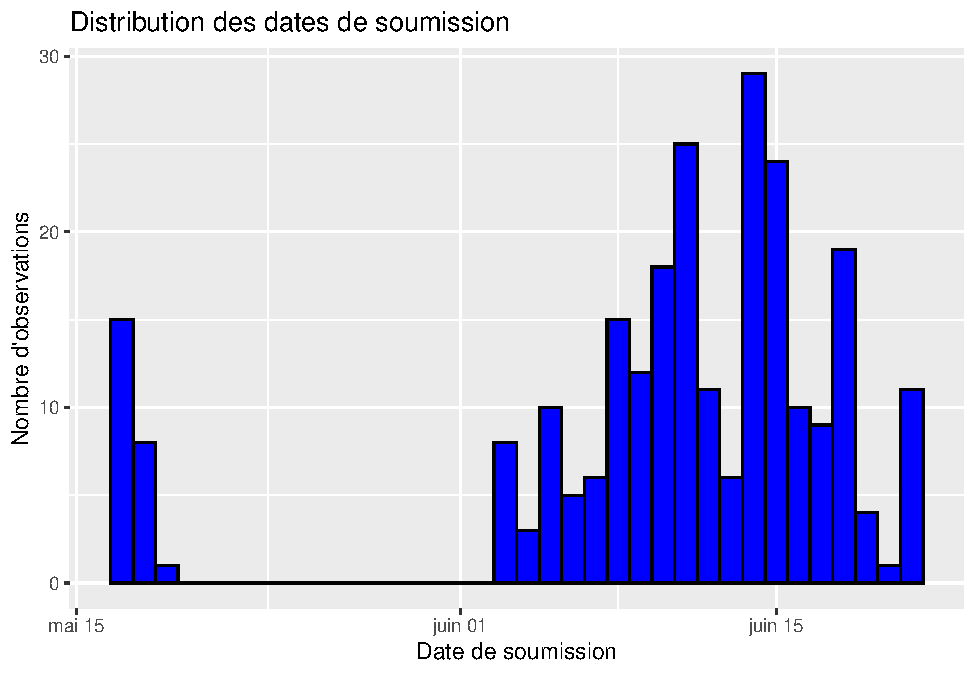
\includegraphics{RMarkdown_files/figure-latex/unnamed-chunk-13-1.pdf}

\begin{Shaded}
\begin{Highlighting}[]
\CommentTok{\# Graphique des dates de début d\textquotesingle{}enregistrement des informations}
\FunctionTok{ggplot}\NormalTok{(data, }\FunctionTok{aes}\NormalTok{(}\AttributeTok{x =}\NormalTok{ start)) }\SpecialCharTok{+}
  \FunctionTok{geom\_histogram}\NormalTok{(}\AttributeTok{binwidth =} \DecValTok{1}\NormalTok{, }\AttributeTok{fill =} \StringTok{"green"}\NormalTok{, }\AttributeTok{color =} \StringTok{"black"}\NormalTok{) }\SpecialCharTok{+}
  \FunctionTok{labs}\NormalTok{(}\AttributeTok{title =} \StringTok{"Dates de début d\textquotesingle{}enregistrement des informations"}\NormalTok{,}
       \AttributeTok{x =} \StringTok{"Date de début d\textquotesingle{}enregistrement"}\NormalTok{,}
       \AttributeTok{y =} \StringTok{"Nombre d\textquotesingle{}observations"}\NormalTok{)}
\end{Highlighting}
\end{Shaded}

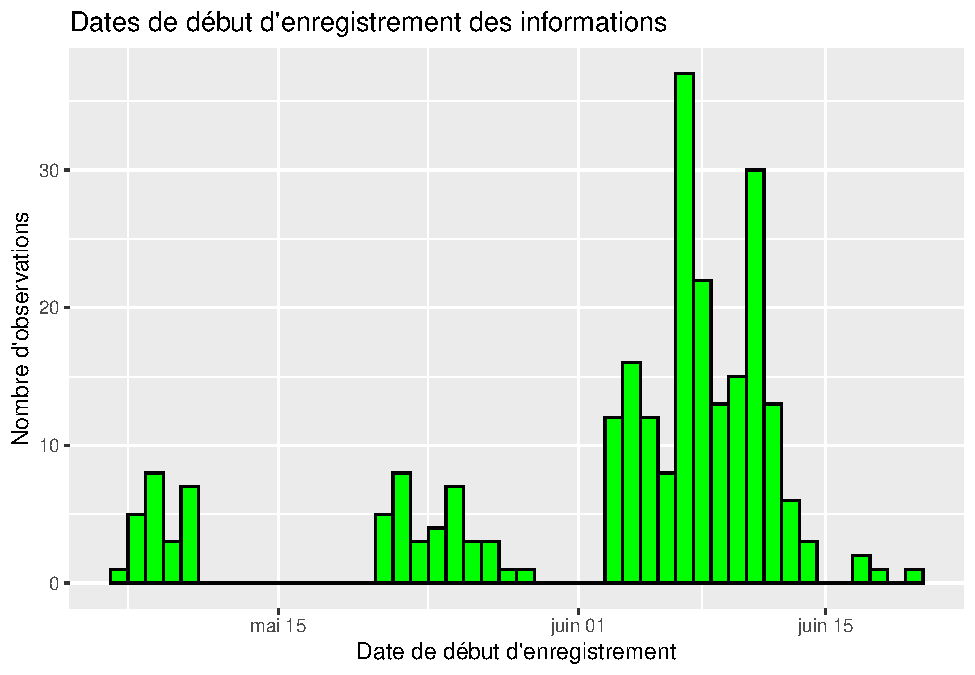
\includegraphics{RMarkdown_files/figure-latex/unnamed-chunk-13-2.pdf}

\begin{Shaded}
\begin{Highlighting}[]
\CommentTok{\# Graphique des dates de l\textquotesingle{}enquête}
\FunctionTok{ggplot}\NormalTok{(data, }\FunctionTok{aes}\NormalTok{(}\AttributeTok{x =}\NormalTok{ today)) }\SpecialCharTok{+}
  \FunctionTok{geom\_histogram}\NormalTok{(}\AttributeTok{binwidth =} \DecValTok{1}\NormalTok{, }\AttributeTok{fill =} \StringTok{"red"}\NormalTok{, }\AttributeTok{color =} \StringTok{"black"}\NormalTok{) }\SpecialCharTok{+}
  \FunctionTok{labs}\NormalTok{(}\AttributeTok{title =} \StringTok{"Dates de l\textquotesingle{}enquête"}\NormalTok{,}
       \AttributeTok{x =} \StringTok{"Date de l\textquotesingle{}enquête"}\NormalTok{,}
       \AttributeTok{y =} \StringTok{"Nombre d\textquotesingle{}observations"}\NormalTok{)}
\end{Highlighting}
\end{Shaded}

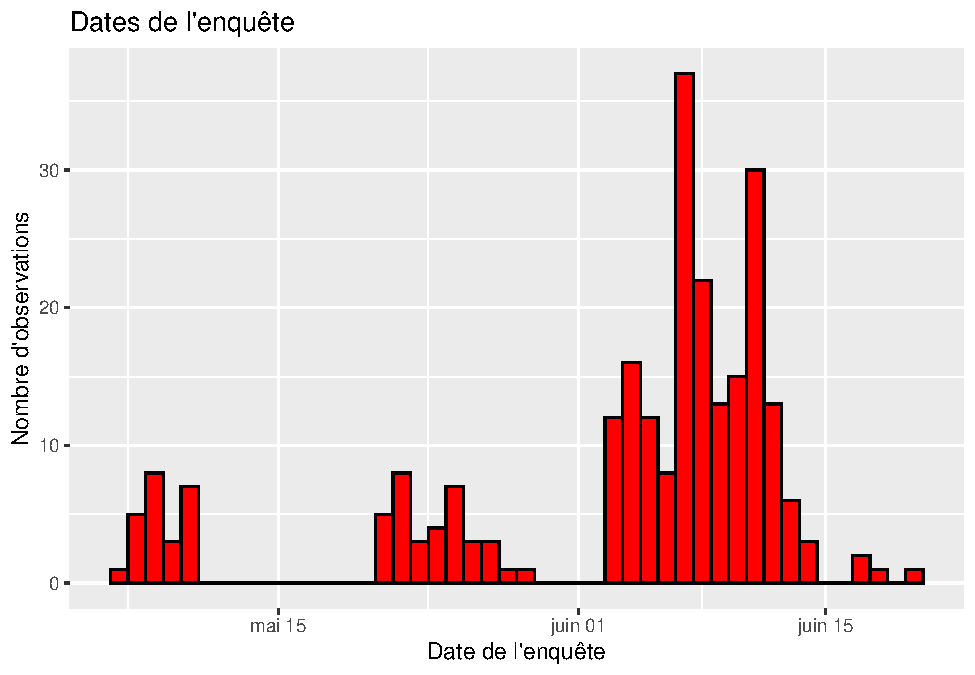
\includegraphics{RMarkdown_files/figure-latex/unnamed-chunk-13-3.pdf}

\begin{Shaded}
\begin{Highlighting}[]
\CommentTok{\# Tableau récapitulatif des dates}
\FunctionTok{tbl\_summary}\NormalTok{(data,}
            \AttributeTok{missing =} \StringTok{"no"}\NormalTok{,}
            \AttributeTok{include =} \FunctionTok{c}\NormalTok{(submissiondate, start, today),}
            \AttributeTok{label=}\FunctionTok{list}\NormalTok{(submissiondate}\SpecialCharTok{\textasciitilde{}} \StringTok{"Date de soumission"}\NormalTok{, }
\NormalTok{                         start}\SpecialCharTok{\textasciitilde{}} \StringTok{"Date de début de l’enrégistrement"}\NormalTok{,}
\NormalTok{                       today}\SpecialCharTok{\textasciitilde{}} \StringTok{"Date de l’enquête"}\NormalTok{)) }\SpecialCharTok{\%\textgreater{}\%} 
  \FunctionTok{modify\_header}\NormalTok{(label }\SpecialCharTok{\textasciitilde{}} \StringTok{"**Date**"}\NormalTok{) }\SpecialCharTok{\%\textgreater{}\%}
  \FunctionTok{italicize\_labels}\NormalTok{() }\SpecialCharTok{\%\textgreater{}\%}
  \FunctionTok{as\_flex\_table}\NormalTok{()}
\end{Highlighting}
\end{Shaded}

\global\setlength{\Oldarrayrulewidth}{\arrayrulewidth}

\global\setlength{\Oldtabcolsep}{\tabcolsep}

\setlength{\tabcolsep}{0pt}

\renewcommand*{\arraystretch}{1.5}



\providecommand{\ascline}[3]{\noalign{\global\arrayrulewidth #1}\arrayrulecolor[HTML]{#2}\cline{#3}}

\begin{longtable}[c]{|p{2.59in}|p{2.06in}}



\ascline{1pt}{000000}{1-2}

\multicolumn{1}{>{\raggedright}m{\dimexpr 2.59in+0\tabcolsep}}{\textcolor[HTML]{000000}{\fontsize{11}{11}\selectfont{\textbf{Date}}}} & \multicolumn{1}{>{\centering}m{\dimexpr 2.06in+0\tabcolsep}}{\textcolor[HTML]{000000}{\fontsize{11}{11}\selectfont{\textbf{N\ =\ 250}}}\textcolor[HTML]{000000}{\textsuperscript{\fontsize{11}{11}\selectfont{1}}}} \\

\ascline{1pt}{000000}{1-2}\endfirsthead 

\ascline{1pt}{000000}{1-2}

\multicolumn{1}{>{\raggedright}m{\dimexpr 2.59in+0\tabcolsep}}{\textcolor[HTML]{000000}{\fontsize{11}{11}\selectfont{\textbf{Date}}}} & \multicolumn{1}{>{\centering}m{\dimexpr 2.06in+0\tabcolsep}}{\textcolor[HTML]{000000}{\fontsize{11}{11}\selectfont{\textbf{N\ =\ 250}}}\textcolor[HTML]{000000}{\textsuperscript{\fontsize{11}{11}\selectfont{1}}}} \\

\ascline{1pt}{000000}{1-2}\endhead



\multicolumn{2}{>{\raggedright}m{\dimexpr 4.65in+2\tabcolsep}}{\textcolor[HTML]{000000}{\textsuperscript{\fontsize{11}{11}\selectfont{1}}}\textcolor[HTML]{000000}{\fontsize{11}{11}\selectfont{Range}}} \\

\endfoot



\multicolumn{1}{>{\raggedright}p{\dimexpr 2.59in+0\tabcolsep}}{\textcolor[HTML]{000000}{\fontsize{11}{11}\selectfont{\textit{Date\ de\ soumission}}}} & \multicolumn{1}{>{\centering}p{\dimexpr 2.06in+0\tabcolsep}}{\textcolor[HTML]{000000}{\fontsize{11}{11}\selectfont{2021-05-17\ to\ 2021-06-21}}} \\





\multicolumn{1}{>{\raggedright}p{\dimexpr 2.59in+0\tabcolsep}}{\textcolor[HTML]{000000}{\fontsize{11}{11}\selectfont{\textit{Date\ de\ début\ de\ l’enrégistrement}}}} & \multicolumn{1}{>{\centering}p{\dimexpr 2.06in+0\tabcolsep}}{\textcolor[HTML]{000000}{\fontsize{11}{11}\selectfont{2021-05-06\ to\ 2021-06-20}}} \\





\multicolumn{1}{>{\raggedright}p{\dimexpr 2.59in+0\tabcolsep}}{\textcolor[HTML]{000000}{\fontsize{11}{11}\selectfont{\textit{Date\ de\ l’enquête}}}} & \multicolumn{1}{>{\centering}p{\dimexpr 2.06in+0\tabcolsep}}{\textcolor[HTML]{000000}{\fontsize{11}{11}\selectfont{2021-05-06\ to\ 2021-06-20}}} \\

\ascline{1pt}{000000}{1-2}



\end{longtable}



\arrayrulecolor[HTML]{000000}

\global\setlength{\arrayrulewidth}{\Oldarrayrulewidth}

\global\setlength{\tabcolsep}{\Oldtabcolsep}

\renewcommand*{\arraystretch}{1}

\textbf{Analyse} :

• La date de soumission varie du 17 mai 2021 au 21 juin 2021 : Cela
indique que les informations de l'enquête ont été soumises sur une
période d'environ un mois.

• La date de début d'enregistrement varie du 6 mai 2021 au 20 juin 2021
: Cela signifie que l'enregistrement des informations pour l'enquête a
commencé à partir du 6 mai 2021 et s'est poursuivi jusqu'au 20 juin
2021.

• La date de l'enquête varie également du 6 mai 2021 au 20 juin 2021 :
Cela indique que les enquêtes ont été menées sur la même période que
l'enregistrement des informations.

\hypertarget{analyse-bivariuxe9e}{%
\paragraph{Analyse bivariée:}\label{analyse-bivariuxe9e}}

\begin{itemize}
\tightlist
\item
  \textbf{Croisement de avec les filières}
\end{itemize}

\begin{Shaded}
\begin{Highlighting}[]
\CommentTok{\# Nous renommons les variables filières aux noms des différents filières}

\CommentTok{\# Nous créeons une fonction croiser\_filiere qui prend en argument}
\CommentTok{\# une filière et renvoie une analyse suivant la filière donnée}
\NormalTok{croiser\_filiere }\OtherTok{\textless{}{-}} \ControlFlowTok{function}\NormalTok{(projet, filiere) \{}
\NormalTok{  tbl\_summary\_result }\OtherTok{\textless{}{-}}\NormalTok{ projet }\SpecialCharTok{\%\textgreater{}\%}
    \FunctionTok{tbl\_summary}\NormalTok{(}
      \AttributeTok{include =} \FunctionTok{c}\NormalTok{(}\StringTok{"sexe"}\NormalTok{, }\StringTok{"region"}\NormalTok{, }\StringTok{"q19"}\NormalTok{),}
      \AttributeTok{by =}\NormalTok{ \{\{ filiere \}\},}
      \AttributeTok{label =} \FunctionTok{list}\NormalTok{(sexe }\SpecialCharTok{\textasciitilde{}} \StringTok{"Sexe"}\NormalTok{,}
\NormalTok{                   region }\SpecialCharTok{\textasciitilde{}} \StringTok{"Region"}\NormalTok{,}
\NormalTok{                   q19 }\SpecialCharTok{\textasciitilde{}} \StringTok{"Etat de la piste qui mène à l’entreprise"}\NormalTok{)}
\NormalTok{    ) }\SpecialCharTok{\%\textgreater{}\%}
    \FunctionTok{modify\_header}\NormalTok{(label }\SpecialCharTok{\textasciitilde{}} \StringTok{"**Variable**"}\NormalTok{) }\SpecialCharTok{\%\textgreater{}\%}
    \FunctionTok{bold\_labels}\NormalTok{()}
  
  \FunctionTok{return}\NormalTok{(tbl\_summary\_result)}
\NormalTok{\}}

\NormalTok{tbl\_filiere\_1 }\OtherTok{\textless{}{-}} \FunctionTok{croiser\_filiere}\NormalTok{(projet2, }\AttributeTok{filiere =} \StringTok{"arachide"}\NormalTok{)}
\NormalTok{tbl\_filiere\_2 }\OtherTok{\textless{}{-}} \FunctionTok{croiser\_filiere}\NormalTok{(projet2, }\AttributeTok{filiere =} \StringTok{"anacarde"}\NormalTok{)}
\NormalTok{tbl\_filiere\_3 }\OtherTok{\textless{}{-}} \FunctionTok{croiser\_filiere}\NormalTok{(projet2, }\AttributeTok{filiere =} \StringTok{"mangue"}\NormalTok{)}
\NormalTok{tbl\_filiere\_4 }\OtherTok{\textless{}{-}} \FunctionTok{croiser\_filiere}\NormalTok{(projet2, }\AttributeTok{filiere =} \StringTok{"riz"}\NormalTok{)}

\FunctionTok{tbl\_merge}\NormalTok{(}
  \FunctionTok{list}\NormalTok{(tbl\_filiere\_1, tbl\_filiere\_2, tbl\_filiere\_3, tbl\_filiere\_4),}
  \AttributeTok{tab\_spanner =} \FunctionTok{c}\NormalTok{(}\StringTok{"arachide"}\NormalTok{, }\StringTok{"anacarde"}\NormalTok{, }\StringTok{"mangue"}\NormalTok{, }\StringTok{"riz"}\NormalTok{)) }\SpecialCharTok{\%\textgreater{}\%}
  \FunctionTok{italicize\_levels}\NormalTok{() }\SpecialCharTok{\%\textgreater{}\%}
  \FunctionTok{as\_flex\_table}\NormalTok{() }\SpecialCharTok{\%\textgreater{}\%}
  \FunctionTok{fontsize}\NormalTok{(}\AttributeTok{size=}\DecValTok{8}\NormalTok{) }\SpecialCharTok{\%\textgreater{}\%}
  \FunctionTok{width}\NormalTok{(}\AttributeTok{width =} \FloatTok{0.8}\NormalTok{ )}
\end{Highlighting}
\end{Shaded}

\global\setlength{\Oldarrayrulewidth}{\arrayrulewidth}

\global\setlength{\Oldtabcolsep}{\tabcolsep}

\setlength{\tabcolsep}{0pt}

\renewcommand*{\arraystretch}{1.5}



\providecommand{\ascline}[3]{\noalign{\global\arrayrulewidth #1}\arrayrulecolor[HTML]{#2}\cline{#3}}

\begin{longtable}[c]{|p{0.80in}|p{0.80in}|p{0.80in}|p{0.80in}|p{0.80in}|p{0.80in}|p{0.80in}|p{0.80in}|p{0.80in}}



\ascline{1pt}{000000}{1-9}

\multicolumn{1}{>{\raggedright}m{\dimexpr 0.8in+0\tabcolsep}}{\textcolor[HTML]{000000}{\fontsize{11}{11}\selectfont{\ }}} & \multicolumn{2}{>{\centering}m{\dimexpr 1.6in+2\tabcolsep}}{\textcolor[HTML]{000000}{\fontsize{11}{11}\selectfont{arachide}}} & \multicolumn{2}{>{\centering}m{\dimexpr 1.6in+2\tabcolsep}}{\textcolor[HTML]{000000}{\fontsize{11}{11}\selectfont{anacarde}}} & \multicolumn{2}{>{\centering}m{\dimexpr 1.6in+2\tabcolsep}}{\textcolor[HTML]{000000}{\fontsize{11}{11}\selectfont{mangue}}} & \multicolumn{2}{>{\centering}m{\dimexpr 1.6in+2\tabcolsep}}{\textcolor[HTML]{000000}{\fontsize{11}{11}\selectfont{riz}}} \\

\ascline{1pt}{000000}{1-9}



\multicolumn{1}{>{\raggedright}m{\dimexpr 0.8in+0\tabcolsep}}{\textcolor[HTML]{000000}{\fontsize{11}{11}\selectfont{\textbf{Variable}}}} & \multicolumn{1}{>{\centering}m{\dimexpr 0.8in+0\tabcolsep}}{\textcolor[HTML]{000000}{\fontsize{11}{11}\selectfont{\textbf{0}}}\textcolor[HTML]{000000}{\fontsize{11}{11}\selectfont{,\ N\ =\ 142}}\textcolor[HTML]{000000}{\textsuperscript{\fontsize{11}{11}\selectfont{1}}}} & \multicolumn{1}{>{\centering}m{\dimexpr 0.8in+0\tabcolsep}}{\textcolor[HTML]{000000}{\fontsize{11}{11}\selectfont{\textbf{1}}}\textcolor[HTML]{000000}{\fontsize{11}{11}\selectfont{,\ N\ =\ 108}}\textcolor[HTML]{000000}{\textsuperscript{\fontsize{11}{11}\selectfont{1}}}} & \multicolumn{1}{>{\centering}m{\dimexpr 0.8in+0\tabcolsep}}{\textcolor[HTML]{000000}{\fontsize{11}{11}\selectfont{\textbf{0}}}\textcolor[HTML]{000000}{\fontsize{11}{11}\selectfont{,\ N\ =\ 189}}\textcolor[HTML]{000000}{\textsuperscript{\fontsize{11}{11}\selectfont{1}}}} & \multicolumn{1}{>{\centering}m{\dimexpr 0.8in+0\tabcolsep}}{\textcolor[HTML]{000000}{\fontsize{11}{11}\selectfont{\textbf{1}}}\textcolor[HTML]{000000}{\fontsize{11}{11}\selectfont{,\ N\ =\ 61}}\textcolor[HTML]{000000}{\textsuperscript{\fontsize{11}{11}\selectfont{1}}}} & \multicolumn{1}{>{\centering}m{\dimexpr 0.8in+0\tabcolsep}}{\textcolor[HTML]{000000}{\fontsize{11}{11}\selectfont{\textbf{0}}}\textcolor[HTML]{000000}{\fontsize{11}{11}\selectfont{,\ N\ =\ 161}}\textcolor[HTML]{000000}{\textsuperscript{\fontsize{11}{11}\selectfont{1}}}} & \multicolumn{1}{>{\centering}m{\dimexpr 0.8in+0\tabcolsep}}{\textcolor[HTML]{000000}{\fontsize{11}{11}\selectfont{\textbf{1}}}\textcolor[HTML]{000000}{\fontsize{11}{11}\selectfont{,\ N\ =\ 89}}\textcolor[HTML]{000000}{\textsuperscript{\fontsize{11}{11}\selectfont{1}}}} & \multicolumn{1}{>{\centering}m{\dimexpr 0.8in+0\tabcolsep}}{\textcolor[HTML]{000000}{\fontsize{11}{11}\selectfont{\textbf{0}}}\textcolor[HTML]{000000}{\fontsize{11}{11}\selectfont{,\ N\ =\ 158}}\textcolor[HTML]{000000}{\textsuperscript{\fontsize{11}{11}\selectfont{1}}}} & \multicolumn{1}{>{\centering}m{\dimexpr 0.8in+0\tabcolsep}}{\textcolor[HTML]{000000}{\fontsize{11}{11}\selectfont{\textbf{1}}}\textcolor[HTML]{000000}{\fontsize{11}{11}\selectfont{,\ N\ =\ 92}}\textcolor[HTML]{000000}{\textsuperscript{\fontsize{11}{11}\selectfont{1}}}} \\

\ascline{1pt}{000000}{1-9}\endfirsthead 

\ascline{1pt}{000000}{1-9}

\multicolumn{1}{>{\raggedright}m{\dimexpr 0.8in+0\tabcolsep}}{\textcolor[HTML]{000000}{\fontsize{11}{11}\selectfont{\ }}} & \multicolumn{2}{>{\centering}m{\dimexpr 1.6in+2\tabcolsep}}{\textcolor[HTML]{000000}{\fontsize{11}{11}\selectfont{arachide}}} & \multicolumn{2}{>{\centering}m{\dimexpr 1.6in+2\tabcolsep}}{\textcolor[HTML]{000000}{\fontsize{11}{11}\selectfont{anacarde}}} & \multicolumn{2}{>{\centering}m{\dimexpr 1.6in+2\tabcolsep}}{\textcolor[HTML]{000000}{\fontsize{11}{11}\selectfont{mangue}}} & \multicolumn{2}{>{\centering}m{\dimexpr 1.6in+2\tabcolsep}}{\textcolor[HTML]{000000}{\fontsize{11}{11}\selectfont{riz}}} \\

\ascline{1pt}{000000}{1-9}



\multicolumn{1}{>{\raggedright}m{\dimexpr 0.8in+0\tabcolsep}}{\textcolor[HTML]{000000}{\fontsize{11}{11}\selectfont{\textbf{Variable}}}} & \multicolumn{1}{>{\centering}m{\dimexpr 0.8in+0\tabcolsep}}{\textcolor[HTML]{000000}{\fontsize{11}{11}\selectfont{\textbf{0}}}\textcolor[HTML]{000000}{\fontsize{11}{11}\selectfont{,\ N\ =\ 142}}\textcolor[HTML]{000000}{\textsuperscript{\fontsize{11}{11}\selectfont{1}}}} & \multicolumn{1}{>{\centering}m{\dimexpr 0.8in+0\tabcolsep}}{\textcolor[HTML]{000000}{\fontsize{11}{11}\selectfont{\textbf{1}}}\textcolor[HTML]{000000}{\fontsize{11}{11}\selectfont{,\ N\ =\ 108}}\textcolor[HTML]{000000}{\textsuperscript{\fontsize{11}{11}\selectfont{1}}}} & \multicolumn{1}{>{\centering}m{\dimexpr 0.8in+0\tabcolsep}}{\textcolor[HTML]{000000}{\fontsize{11}{11}\selectfont{\textbf{0}}}\textcolor[HTML]{000000}{\fontsize{11}{11}\selectfont{,\ N\ =\ 189}}\textcolor[HTML]{000000}{\textsuperscript{\fontsize{11}{11}\selectfont{1}}}} & \multicolumn{1}{>{\centering}m{\dimexpr 0.8in+0\tabcolsep}}{\textcolor[HTML]{000000}{\fontsize{11}{11}\selectfont{\textbf{1}}}\textcolor[HTML]{000000}{\fontsize{11}{11}\selectfont{,\ N\ =\ 61}}\textcolor[HTML]{000000}{\textsuperscript{\fontsize{11}{11}\selectfont{1}}}} & \multicolumn{1}{>{\centering}m{\dimexpr 0.8in+0\tabcolsep}}{\textcolor[HTML]{000000}{\fontsize{11}{11}\selectfont{\textbf{0}}}\textcolor[HTML]{000000}{\fontsize{11}{11}\selectfont{,\ N\ =\ 161}}\textcolor[HTML]{000000}{\textsuperscript{\fontsize{11}{11}\selectfont{1}}}} & \multicolumn{1}{>{\centering}m{\dimexpr 0.8in+0\tabcolsep}}{\textcolor[HTML]{000000}{\fontsize{11}{11}\selectfont{\textbf{1}}}\textcolor[HTML]{000000}{\fontsize{11}{11}\selectfont{,\ N\ =\ 89}}\textcolor[HTML]{000000}{\textsuperscript{\fontsize{11}{11}\selectfont{1}}}} & \multicolumn{1}{>{\centering}m{\dimexpr 0.8in+0\tabcolsep}}{\textcolor[HTML]{000000}{\fontsize{11}{11}\selectfont{\textbf{0}}}\textcolor[HTML]{000000}{\fontsize{11}{11}\selectfont{,\ N\ =\ 158}}\textcolor[HTML]{000000}{\textsuperscript{\fontsize{11}{11}\selectfont{1}}}} & \multicolumn{1}{>{\centering}m{\dimexpr 0.8in+0\tabcolsep}}{\textcolor[HTML]{000000}{\fontsize{11}{11}\selectfont{\textbf{1}}}\textcolor[HTML]{000000}{\fontsize{11}{11}\selectfont{,\ N\ =\ 92}}\textcolor[HTML]{000000}{\textsuperscript{\fontsize{11}{11}\selectfont{1}}}} \\

\ascline{1pt}{000000}{1-9}\endhead



\multicolumn{9}{>{\raggedright}m{\dimexpr 7.2in+16\tabcolsep}}{\textcolor[HTML]{000000}{\textsuperscript{\fontsize{11}{11}\selectfont{1}}}\textcolor[HTML]{000000}{\fontsize{11}{11}\selectfont{n\ (\%)}}} \\

\endfoot



\multicolumn{1}{>{\raggedright}p{\dimexpr 0.8in+0\tabcolsep}}{\textcolor[HTML]{000000}{\fontsize{8}{8}\selectfont{\textbf{Sexe}}}} & \multicolumn{1}{>{\centering}p{\dimexpr 0.8in+0\tabcolsep}}{\textcolor[HTML]{000000}{\fontsize{8}{8}\selectfont{}}} & \multicolumn{1}{>{\centering}p{\dimexpr 0.8in+0\tabcolsep}}{\textcolor[HTML]{000000}{\fontsize{8}{8}\selectfont{}}} & \multicolumn{1}{>{\centering}p{\dimexpr 0.8in+0\tabcolsep}}{\textcolor[HTML]{000000}{\fontsize{8}{8}\selectfont{}}} & \multicolumn{1}{>{\centering}p{\dimexpr 0.8in+0\tabcolsep}}{\textcolor[HTML]{000000}{\fontsize{8}{8}\selectfont{}}} & \multicolumn{1}{>{\centering}p{\dimexpr 0.8in+0\tabcolsep}}{\textcolor[HTML]{000000}{\fontsize{8}{8}\selectfont{}}} & \multicolumn{1}{>{\centering}p{\dimexpr 0.8in+0\tabcolsep}}{\textcolor[HTML]{000000}{\fontsize{8}{8}\selectfont{}}} & \multicolumn{1}{>{\centering}p{\dimexpr 0.8in+0\tabcolsep}}{\textcolor[HTML]{000000}{\fontsize{8}{8}\selectfont{}}} & \multicolumn{1}{>{\centering}p{\dimexpr 0.8in+0\tabcolsep}}{\textcolor[HTML]{000000}{\fontsize{8}{8}\selectfont{}}} \\





\multicolumn{1}{>{\raggedright}p{\dimexpr 0.8in+0\tabcolsep}}{\textcolor[HTML]{000000}{\fontsize{8}{8}\selectfont{\textit{Femme}}}} & \multicolumn{1}{>{\centering}p{\dimexpr 0.8in+0\tabcolsep}}{\textcolor[HTML]{000000}{\fontsize{8}{8}\selectfont{98\ (69\%)}}} & \multicolumn{1}{>{\centering}p{\dimexpr 0.8in+0\tabcolsep}}{\textcolor[HTML]{000000}{\fontsize{8}{8}\selectfont{93\ (86\%)}}} & \multicolumn{1}{>{\centering}p{\dimexpr 0.8in+0\tabcolsep}}{\textcolor[HTML]{000000}{\fontsize{8}{8}\selectfont{151\ (80\%)}}} & \multicolumn{1}{>{\centering}p{\dimexpr 0.8in+0\tabcolsep}}{\textcolor[HTML]{000000}{\fontsize{8}{8}\selectfont{40\ (66\%)}}} & \multicolumn{1}{>{\centering}p{\dimexpr 0.8in+0\tabcolsep}}{\textcolor[HTML]{000000}{\fontsize{8}{8}\selectfont{123\ (76\%)}}} & \multicolumn{1}{>{\centering}p{\dimexpr 0.8in+0\tabcolsep}}{\textcolor[HTML]{000000}{\fontsize{8}{8}\selectfont{68\ (76\%)}}} & \multicolumn{1}{>{\centering}p{\dimexpr 0.8in+0\tabcolsep}}{\textcolor[HTML]{000000}{\fontsize{8}{8}\selectfont{114\ (72\%)}}} & \multicolumn{1}{>{\centering}p{\dimexpr 0.8in+0\tabcolsep}}{\textcolor[HTML]{000000}{\fontsize{8}{8}\selectfont{77\ (84\%)}}} \\





\multicolumn{1}{>{\raggedright}p{\dimexpr 0.8in+0\tabcolsep}}{\textcolor[HTML]{000000}{\fontsize{8}{8}\selectfont{\textit{Homme}}}} & \multicolumn{1}{>{\centering}p{\dimexpr 0.8in+0\tabcolsep}}{\textcolor[HTML]{000000}{\fontsize{8}{8}\selectfont{44\ (31\%)}}} & \multicolumn{1}{>{\centering}p{\dimexpr 0.8in+0\tabcolsep}}{\textcolor[HTML]{000000}{\fontsize{8}{8}\selectfont{15\ (14\%)}}} & \multicolumn{1}{>{\centering}p{\dimexpr 0.8in+0\tabcolsep}}{\textcolor[HTML]{000000}{\fontsize{8}{8}\selectfont{38\ (20\%)}}} & \multicolumn{1}{>{\centering}p{\dimexpr 0.8in+0\tabcolsep}}{\textcolor[HTML]{000000}{\fontsize{8}{8}\selectfont{21\ (34\%)}}} & \multicolumn{1}{>{\centering}p{\dimexpr 0.8in+0\tabcolsep}}{\textcolor[HTML]{000000}{\fontsize{8}{8}\selectfont{38\ (24\%)}}} & \multicolumn{1}{>{\centering}p{\dimexpr 0.8in+0\tabcolsep}}{\textcolor[HTML]{000000}{\fontsize{8}{8}\selectfont{21\ (24\%)}}} & \multicolumn{1}{>{\centering}p{\dimexpr 0.8in+0\tabcolsep}}{\textcolor[HTML]{000000}{\fontsize{8}{8}\selectfont{44\ (28\%)}}} & \multicolumn{1}{>{\centering}p{\dimexpr 0.8in+0\tabcolsep}}{\textcolor[HTML]{000000}{\fontsize{8}{8}\selectfont{15\ (16\%)}}} \\





\multicolumn{1}{>{\raggedright}p{\dimexpr 0.8in+0\tabcolsep}}{\textcolor[HTML]{000000}{\fontsize{8}{8}\selectfont{\textbf{Region}}}} & \multicolumn{1}{>{\centering}p{\dimexpr 0.8in+0\tabcolsep}}{\textcolor[HTML]{000000}{\fontsize{8}{8}\selectfont{}}} & \multicolumn{1}{>{\centering}p{\dimexpr 0.8in+0\tabcolsep}}{\textcolor[HTML]{000000}{\fontsize{8}{8}\selectfont{}}} & \multicolumn{1}{>{\centering}p{\dimexpr 0.8in+0\tabcolsep}}{\textcolor[HTML]{000000}{\fontsize{8}{8}\selectfont{}}} & \multicolumn{1}{>{\centering}p{\dimexpr 0.8in+0\tabcolsep}}{\textcolor[HTML]{000000}{\fontsize{8}{8}\selectfont{}}} & \multicolumn{1}{>{\centering}p{\dimexpr 0.8in+0\tabcolsep}}{\textcolor[HTML]{000000}{\fontsize{8}{8}\selectfont{}}} & \multicolumn{1}{>{\centering}p{\dimexpr 0.8in+0\tabcolsep}}{\textcolor[HTML]{000000}{\fontsize{8}{8}\selectfont{}}} & \multicolumn{1}{>{\centering}p{\dimexpr 0.8in+0\tabcolsep}}{\textcolor[HTML]{000000}{\fontsize{8}{8}\selectfont{}}} & \multicolumn{1}{>{\centering}p{\dimexpr 0.8in+0\tabcolsep}}{\textcolor[HTML]{000000}{\fontsize{8}{8}\selectfont{}}} \\





\multicolumn{1}{>{\raggedright}p{\dimexpr 0.8in+0\tabcolsep}}{\textcolor[HTML]{000000}{\fontsize{8}{8}\selectfont{\textit{Dakar}}}} & \multicolumn{1}{>{\centering}p{\dimexpr 0.8in+0\tabcolsep}}{\textcolor[HTML]{000000}{\fontsize{8}{8}\selectfont{1\ (0.7\%)}}} & \multicolumn{1}{>{\centering}p{\dimexpr 0.8in+0\tabcolsep}}{\textcolor[HTML]{000000}{\fontsize{8}{8}\selectfont{0\ (0\%)}}} & \multicolumn{1}{>{\centering}p{\dimexpr 0.8in+0\tabcolsep}}{\textcolor[HTML]{000000}{\fontsize{8}{8}\selectfont{0\ (0\%)}}} & \multicolumn{1}{>{\centering}p{\dimexpr 0.8in+0\tabcolsep}}{\textcolor[HTML]{000000}{\fontsize{8}{8}\selectfont{1\ (1.6\%)}}} & \multicolumn{1}{>{\centering}p{\dimexpr 0.8in+0\tabcolsep}}{\textcolor[HTML]{000000}{\fontsize{8}{8}\selectfont{1\ (0.6\%)}}} & \multicolumn{1}{>{\centering}p{\dimexpr 0.8in+0\tabcolsep}}{\textcolor[HTML]{000000}{\fontsize{8}{8}\selectfont{0\ (0\%)}}} & \multicolumn{1}{>{\centering}p{\dimexpr 0.8in+0\tabcolsep}}{\textcolor[HTML]{000000}{\fontsize{8}{8}\selectfont{0\ (0\%)}}} & \multicolumn{1}{>{\centering}p{\dimexpr 0.8in+0\tabcolsep}}{\textcolor[HTML]{000000}{\fontsize{8}{8}\selectfont{1\ (1.1\%)}}} \\





\multicolumn{1}{>{\raggedright}p{\dimexpr 0.8in+0\tabcolsep}}{\textcolor[HTML]{000000}{\fontsize{8}{8}\selectfont{\textit{Diourbel}}}} & \multicolumn{1}{>{\centering}p{\dimexpr 0.8in+0\tabcolsep}}{\textcolor[HTML]{000000}{\fontsize{8}{8}\selectfont{1\ (0.7\%)}}} & \multicolumn{1}{>{\centering}p{\dimexpr 0.8in+0\tabcolsep}}{\textcolor[HTML]{000000}{\fontsize{8}{8}\selectfont{33\ (31\%)}}} & \multicolumn{1}{>{\centering}p{\dimexpr 0.8in+0\tabcolsep}}{\textcolor[HTML]{000000}{\fontsize{8}{8}\selectfont{34\ (18\%)}}} & \multicolumn{1}{>{\centering}p{\dimexpr 0.8in+0\tabcolsep}}{\textcolor[HTML]{000000}{\fontsize{8}{8}\selectfont{0\ (0\%)}}} & \multicolumn{1}{>{\centering}p{\dimexpr 0.8in+0\tabcolsep}}{\textcolor[HTML]{000000}{\fontsize{8}{8}\selectfont{33\ (20\%)}}} & \multicolumn{1}{>{\centering}p{\dimexpr 0.8in+0\tabcolsep}}{\textcolor[HTML]{000000}{\fontsize{8}{8}\selectfont{1\ (1.1\%)}}} & \multicolumn{1}{>{\centering}p{\dimexpr 0.8in+0\tabcolsep}}{\textcolor[HTML]{000000}{\fontsize{8}{8}\selectfont{34\ (22\%)}}} & \multicolumn{1}{>{\centering}p{\dimexpr 0.8in+0\tabcolsep}}{\textcolor[HTML]{000000}{\fontsize{8}{8}\selectfont{0\ (0\%)}}} \\





\multicolumn{1}{>{\raggedright}p{\dimexpr 0.8in+0\tabcolsep}}{\textcolor[HTML]{000000}{\fontsize{8}{8}\selectfont{\textit{Fatick}}}} & \multicolumn{1}{>{\centering}p{\dimexpr 0.8in+0\tabcolsep}}{\textcolor[HTML]{000000}{\fontsize{8}{8}\selectfont{18\ (13\%)}}} & \multicolumn{1}{>{\centering}p{\dimexpr 0.8in+0\tabcolsep}}{\textcolor[HTML]{000000}{\fontsize{8}{8}\selectfont{12\ (11\%)}}} & \multicolumn{1}{>{\centering}p{\dimexpr 0.8in+0\tabcolsep}}{\textcolor[HTML]{000000}{\fontsize{8}{8}\selectfont{9\ (4.8\%)}}} & \multicolumn{1}{>{\centering}p{\dimexpr 0.8in+0\tabcolsep}}{\textcolor[HTML]{000000}{\fontsize{8}{8}\selectfont{21\ (34\%)}}} & \multicolumn{1}{>{\centering}p{\dimexpr 0.8in+0\tabcolsep}}{\textcolor[HTML]{000000}{\fontsize{8}{8}\selectfont{27\ (17\%)}}} & \multicolumn{1}{>{\centering}p{\dimexpr 0.8in+0\tabcolsep}}{\textcolor[HTML]{000000}{\fontsize{8}{8}\selectfont{3\ (3.4\%)}}} & \multicolumn{1}{>{\centering}p{\dimexpr 0.8in+0\tabcolsep}}{\textcolor[HTML]{000000}{\fontsize{8}{8}\selectfont{26\ (16\%)}}} & \multicolumn{1}{>{\centering}p{\dimexpr 0.8in+0\tabcolsep}}{\textcolor[HTML]{000000}{\fontsize{8}{8}\selectfont{4\ (4.3\%)}}} \\





\multicolumn{1}{>{\raggedright}p{\dimexpr 0.8in+0\tabcolsep}}{\textcolor[HTML]{000000}{\fontsize{8}{8}\selectfont{\textit{Kaffrine}}}} & \multicolumn{1}{>{\centering}p{\dimexpr 0.8in+0\tabcolsep}}{\textcolor[HTML]{000000}{\fontsize{8}{8}\selectfont{0\ (0\%)}}} & \multicolumn{1}{>{\centering}p{\dimexpr 0.8in+0\tabcolsep}}{\textcolor[HTML]{000000}{\fontsize{8}{8}\selectfont{8\ (7.4\%)}}} & \multicolumn{1}{>{\centering}p{\dimexpr 0.8in+0\tabcolsep}}{\textcolor[HTML]{000000}{\fontsize{8}{8}\selectfont{8\ (4.2\%)}}} & \multicolumn{1}{>{\centering}p{\dimexpr 0.8in+0\tabcolsep}}{\textcolor[HTML]{000000}{\fontsize{8}{8}\selectfont{0\ (0\%)}}} & \multicolumn{1}{>{\centering}p{\dimexpr 0.8in+0\tabcolsep}}{\textcolor[HTML]{000000}{\fontsize{8}{8}\selectfont{3\ (1.9\%)}}} & \multicolumn{1}{>{\centering}p{\dimexpr 0.8in+0\tabcolsep}}{\textcolor[HTML]{000000}{\fontsize{8}{8}\selectfont{5\ (5.6\%)}}} & \multicolumn{1}{>{\centering}p{\dimexpr 0.8in+0\tabcolsep}}{\textcolor[HTML]{000000}{\fontsize{8}{8}\selectfont{7\ (4.4\%)}}} & \multicolumn{1}{>{\centering}p{\dimexpr 0.8in+0\tabcolsep}}{\textcolor[HTML]{000000}{\fontsize{8}{8}\selectfont{1\ (1.1\%)}}} \\





\multicolumn{1}{>{\raggedright}p{\dimexpr 0.8in+0\tabcolsep}}{\textcolor[HTML]{000000}{\fontsize{8}{8}\selectfont{\textit{Kaolack}}}} & \multicolumn{1}{>{\centering}p{\dimexpr 0.8in+0\tabcolsep}}{\textcolor[HTML]{000000}{\fontsize{8}{8}\selectfont{1\ (0.7\%)}}} & \multicolumn{1}{>{\centering}p{\dimexpr 0.8in+0\tabcolsep}}{\textcolor[HTML]{000000}{\fontsize{8}{8}\selectfont{20\ (19\%)}}} & \multicolumn{1}{>{\centering}p{\dimexpr 0.8in+0\tabcolsep}}{\textcolor[HTML]{000000}{\fontsize{8}{8}\selectfont{21\ (11\%)}}} & \multicolumn{1}{>{\centering}p{\dimexpr 0.8in+0\tabcolsep}}{\textcolor[HTML]{000000}{\fontsize{8}{8}\selectfont{0\ (0\%)}}} & \multicolumn{1}{>{\centering}p{\dimexpr 0.8in+0\tabcolsep}}{\textcolor[HTML]{000000}{\fontsize{8}{8}\selectfont{14\ (8.7\%)}}} & \multicolumn{1}{>{\centering}p{\dimexpr 0.8in+0\tabcolsep}}{\textcolor[HTML]{000000}{\fontsize{8}{8}\selectfont{7\ (7.9\%)}}} & \multicolumn{1}{>{\centering}p{\dimexpr 0.8in+0\tabcolsep}}{\textcolor[HTML]{000000}{\fontsize{8}{8}\selectfont{17\ (11\%)}}} & \multicolumn{1}{>{\centering}p{\dimexpr 0.8in+0\tabcolsep}}{\textcolor[HTML]{000000}{\fontsize{8}{8}\selectfont{4\ (4.3\%)}}} \\





\multicolumn{1}{>{\raggedright}p{\dimexpr 0.8in+0\tabcolsep}}{\textcolor[HTML]{000000}{\fontsize{8}{8}\selectfont{\textit{Kolda}}}} & \multicolumn{1}{>{\centering}p{\dimexpr 0.8in+0\tabcolsep}}{\textcolor[HTML]{000000}{\fontsize{8}{8}\selectfont{8\ (5.6\%)}}} & \multicolumn{1}{>{\centering}p{\dimexpr 0.8in+0\tabcolsep}}{\textcolor[HTML]{000000}{\fontsize{8}{8}\selectfont{1\ (0.9\%)}}} & \multicolumn{1}{>{\centering}p{\dimexpr 0.8in+0\tabcolsep}}{\textcolor[HTML]{000000}{\fontsize{8}{8}\selectfont{4\ (2.1\%)}}} & \multicolumn{1}{>{\centering}p{\dimexpr 0.8in+0\tabcolsep}}{\textcolor[HTML]{000000}{\fontsize{8}{8}\selectfont{5\ (8.2\%)}}} & \multicolumn{1}{>{\centering}p{\dimexpr 0.8in+0\tabcolsep}}{\textcolor[HTML]{000000}{\fontsize{8}{8}\selectfont{9\ (5.6\%)}}} & \multicolumn{1}{>{\centering}p{\dimexpr 0.8in+0\tabcolsep}}{\textcolor[HTML]{000000}{\fontsize{8}{8}\selectfont{0\ (0\%)}}} & \multicolumn{1}{>{\centering}p{\dimexpr 0.8in+0\tabcolsep}}{\textcolor[HTML]{000000}{\fontsize{8}{8}\selectfont{5\ (3.2\%)}}} & \multicolumn{1}{>{\centering}p{\dimexpr 0.8in+0\tabcolsep}}{\textcolor[HTML]{000000}{\fontsize{8}{8}\selectfont{4\ (4.3\%)}}} \\





\multicolumn{1}{>{\raggedright}p{\dimexpr 0.8in+0\tabcolsep}}{\textcolor[HTML]{000000}{\fontsize{8}{8}\selectfont{\textit{Saint-Louis}}}} & \multicolumn{1}{>{\centering}p{\dimexpr 0.8in+0\tabcolsep}}{\textcolor[HTML]{000000}{\fontsize{8}{8}\selectfont{41\ (29\%)}}} & \multicolumn{1}{>{\centering}p{\dimexpr 0.8in+0\tabcolsep}}{\textcolor[HTML]{000000}{\fontsize{8}{8}\selectfont{1\ (0.9\%)}}} & \multicolumn{1}{>{\centering}p{\dimexpr 0.8in+0\tabcolsep}}{\textcolor[HTML]{000000}{\fontsize{8}{8}\selectfont{42\ (22\%)}}} & \multicolumn{1}{>{\centering}p{\dimexpr 0.8in+0\tabcolsep}}{\textcolor[HTML]{000000}{\fontsize{8}{8}\selectfont{0\ (0\%)}}} & \multicolumn{1}{>{\centering}p{\dimexpr 0.8in+0\tabcolsep}}{\textcolor[HTML]{000000}{\fontsize{8}{8}\selectfont{0\ (0\%)}}} & \multicolumn{1}{>{\centering}p{\dimexpr 0.8in+0\tabcolsep}}{\textcolor[HTML]{000000}{\fontsize{8}{8}\selectfont{42\ (47\%)}}} & \multicolumn{1}{>{\centering}p{\dimexpr 0.8in+0\tabcolsep}}{\textcolor[HTML]{000000}{\fontsize{8}{8}\selectfont{42\ (27\%)}}} & \multicolumn{1}{>{\centering}p{\dimexpr 0.8in+0\tabcolsep}}{\textcolor[HTML]{000000}{\fontsize{8}{8}\selectfont{0\ (0\%)}}} \\





\multicolumn{1}{>{\raggedright}p{\dimexpr 0.8in+0\tabcolsep}}{\textcolor[HTML]{000000}{\fontsize{8}{8}\selectfont{\textit{Sédhiou}}}} & \multicolumn{1}{>{\centering}p{\dimexpr 0.8in+0\tabcolsep}}{\textcolor[HTML]{000000}{\fontsize{8}{8}\selectfont{4\ (2.8\%)}}} & \multicolumn{1}{>{\centering}p{\dimexpr 0.8in+0\tabcolsep}}{\textcolor[HTML]{000000}{\fontsize{8}{8}\selectfont{0\ (0\%)}}} & \multicolumn{1}{>{\centering}p{\dimexpr 0.8in+0\tabcolsep}}{\textcolor[HTML]{000000}{\fontsize{8}{8}\selectfont{1\ (0.5\%)}}} & \multicolumn{1}{>{\centering}p{\dimexpr 0.8in+0\tabcolsep}}{\textcolor[HTML]{000000}{\fontsize{8}{8}\selectfont{3\ (4.9\%)}}} & \multicolumn{1}{>{\centering}p{\dimexpr 0.8in+0\tabcolsep}}{\textcolor[HTML]{000000}{\fontsize{8}{8}\selectfont{4\ (2.5\%)}}} & \multicolumn{1}{>{\centering}p{\dimexpr 0.8in+0\tabcolsep}}{\textcolor[HTML]{000000}{\fontsize{8}{8}\selectfont{0\ (0\%)}}} & \multicolumn{1}{>{\centering}p{\dimexpr 0.8in+0\tabcolsep}}{\textcolor[HTML]{000000}{\fontsize{8}{8}\selectfont{1\ (0.6\%)}}} & \multicolumn{1}{>{\centering}p{\dimexpr 0.8in+0\tabcolsep}}{\textcolor[HTML]{000000}{\fontsize{8}{8}\selectfont{3\ (3.3\%)}}} \\





\multicolumn{1}{>{\raggedright}p{\dimexpr 0.8in+0\tabcolsep}}{\textcolor[HTML]{000000}{\fontsize{8}{8}\selectfont{\textit{Thiès}}}} & \multicolumn{1}{>{\centering}p{\dimexpr 0.8in+0\tabcolsep}}{\textcolor[HTML]{000000}{\fontsize{8}{8}\selectfont{24\ (17\%)}}} & \multicolumn{1}{>{\centering}p{\dimexpr 0.8in+0\tabcolsep}}{\textcolor[HTML]{000000}{\fontsize{8}{8}\selectfont{27\ (25\%)}}} & \multicolumn{1}{>{\centering}p{\dimexpr 0.8in+0\tabcolsep}}{\textcolor[HTML]{000000}{\fontsize{8}{8}\selectfont{51\ (27\%)}}} & \multicolumn{1}{>{\centering}p{\dimexpr 0.8in+0\tabcolsep}}{\textcolor[HTML]{000000}{\fontsize{8}{8}\selectfont{0\ (0\%)}}} & \multicolumn{1}{>{\centering}p{\dimexpr 0.8in+0\tabcolsep}}{\textcolor[HTML]{000000}{\fontsize{8}{8}\selectfont{26\ (16\%)}}} & \multicolumn{1}{>{\centering}p{\dimexpr 0.8in+0\tabcolsep}}{\textcolor[HTML]{000000}{\fontsize{8}{8}\selectfont{25\ (28\%)}}} & \multicolumn{1}{>{\centering}p{\dimexpr 0.8in+0\tabcolsep}}{\textcolor[HTML]{000000}{\fontsize{8}{8}\selectfont{19\ (12\%)}}} & \multicolumn{1}{>{\centering}p{\dimexpr 0.8in+0\tabcolsep}}{\textcolor[HTML]{000000}{\fontsize{8}{8}\selectfont{32\ (35\%)}}} \\





\multicolumn{1}{>{\raggedright}p{\dimexpr 0.8in+0\tabcolsep}}{\textcolor[HTML]{000000}{\fontsize{8}{8}\selectfont{\textit{Ziguinchor}}}} & \multicolumn{1}{>{\centering}p{\dimexpr 0.8in+0\tabcolsep}}{\textcolor[HTML]{000000}{\fontsize{8}{8}\selectfont{44\ (31\%)}}} & \multicolumn{1}{>{\centering}p{\dimexpr 0.8in+0\tabcolsep}}{\textcolor[HTML]{000000}{\fontsize{8}{8}\selectfont{6\ (5.6\%)}}} & \multicolumn{1}{>{\centering}p{\dimexpr 0.8in+0\tabcolsep}}{\textcolor[HTML]{000000}{\fontsize{8}{8}\selectfont{19\ (10\%)}}} & \multicolumn{1}{>{\centering}p{\dimexpr 0.8in+0\tabcolsep}}{\textcolor[HTML]{000000}{\fontsize{8}{8}\selectfont{31\ (51\%)}}} & \multicolumn{1}{>{\centering}p{\dimexpr 0.8in+0\tabcolsep}}{\textcolor[HTML]{000000}{\fontsize{8}{8}\selectfont{44\ (27\%)}}} & \multicolumn{1}{>{\centering}p{\dimexpr 0.8in+0\tabcolsep}}{\textcolor[HTML]{000000}{\fontsize{8}{8}\selectfont{6\ (6.7\%)}}} & \multicolumn{1}{>{\centering}p{\dimexpr 0.8in+0\tabcolsep}}{\textcolor[HTML]{000000}{\fontsize{8}{8}\selectfont{7\ (4.4\%)}}} & \multicolumn{1}{>{\centering}p{\dimexpr 0.8in+0\tabcolsep}}{\textcolor[HTML]{000000}{\fontsize{8}{8}\selectfont{43\ (47\%)}}} \\





\multicolumn{1}{>{\raggedright}p{\dimexpr 0.8in+0\tabcolsep}}{\textcolor[HTML]{000000}{\fontsize{8}{8}\selectfont{\textbf{Etat\ de\ la\ piste\ qui\ mène\ à\ l’entreprise}}}} & \multicolumn{1}{>{\centering}p{\dimexpr 0.8in+0\tabcolsep}}{\textcolor[HTML]{000000}{\fontsize{8}{8}\selectfont{}}} & \multicolumn{1}{>{\centering}p{\dimexpr 0.8in+0\tabcolsep}}{\textcolor[HTML]{000000}{\fontsize{8}{8}\selectfont{}}} & \multicolumn{1}{>{\centering}p{\dimexpr 0.8in+0\tabcolsep}}{\textcolor[HTML]{000000}{\fontsize{8}{8}\selectfont{}}} & \multicolumn{1}{>{\centering}p{\dimexpr 0.8in+0\tabcolsep}}{\textcolor[HTML]{000000}{\fontsize{8}{8}\selectfont{}}} & \multicolumn{1}{>{\centering}p{\dimexpr 0.8in+0\tabcolsep}}{\textcolor[HTML]{000000}{\fontsize{8}{8}\selectfont{}}} & \multicolumn{1}{>{\centering}p{\dimexpr 0.8in+0\tabcolsep}}{\textcolor[HTML]{000000}{\fontsize{8}{8}\selectfont{}}} & \multicolumn{1}{>{\centering}p{\dimexpr 0.8in+0\tabcolsep}}{\textcolor[HTML]{000000}{\fontsize{8}{8}\selectfont{}}} & \multicolumn{1}{>{\centering}p{\dimexpr 0.8in+0\tabcolsep}}{\textcolor[HTML]{000000}{\fontsize{8}{8}\selectfont{}}} \\





\multicolumn{1}{>{\raggedright}p{\dimexpr 0.8in+0\tabcolsep}}{\textcolor[HTML]{000000}{\fontsize{8}{8}\selectfont{\textit{Bon\ état}}}} & \multicolumn{1}{>{\centering}p{\dimexpr 0.8in+0\tabcolsep}}{\textcolor[HTML]{000000}{\fontsize{8}{8}\selectfont{2\ (3.2\%)}}} & \multicolumn{1}{>{\centering}p{\dimexpr 0.8in+0\tabcolsep}}{\textcolor[HTML]{000000}{\fontsize{8}{8}\selectfont{0\ (0\%)}}} & \multicolumn{1}{>{\centering}p{\dimexpr 0.8in+0\tabcolsep}}{\textcolor[HTML]{000000}{\fontsize{8}{8}\selectfont{1\ (1.0\%)}}} & \multicolumn{1}{>{\centering}p{\dimexpr 0.8in+0\tabcolsep}}{\textcolor[HTML]{000000}{\fontsize{8}{8}\selectfont{1\ (2.9\%)}}} & \multicolumn{1}{>{\centering}p{\dimexpr 0.8in+0\tabcolsep}}{\textcolor[HTML]{000000}{\fontsize{8}{8}\selectfont{2\ (2.1\%)}}} & \multicolumn{1}{>{\centering}p{\dimexpr 0.8in+0\tabcolsep}}{\textcolor[HTML]{000000}{\fontsize{8}{8}\selectfont{0\ (0\%)}}} & \multicolumn{1}{>{\centering}p{\dimexpr 0.8in+0\tabcolsep}}{\textcolor[HTML]{000000}{\fontsize{8}{8}\selectfont{0\ (0\%)}}} & \multicolumn{1}{>{\centering}p{\dimexpr 0.8in+0\tabcolsep}}{\textcolor[HTML]{000000}{\fontsize{8}{8}\selectfont{2\ (4.5\%)}}} \\





\multicolumn{1}{>{\raggedright}p{\dimexpr 0.8in+0\tabcolsep}}{\textcolor[HTML]{000000}{\fontsize{8}{8}\selectfont{\textit{Etat\ moyen}}}} & \multicolumn{1}{>{\centering}p{\dimexpr 0.8in+0\tabcolsep}}{\textcolor[HTML]{000000}{\fontsize{8}{8}\selectfont{35\ (56\%)}}} & \multicolumn{1}{>{\centering}p{\dimexpr 0.8in+0\tabcolsep}}{\textcolor[HTML]{000000}{\fontsize{8}{8}\selectfont{38\ (57\%)}}} & \multicolumn{1}{>{\centering}p{\dimexpr 0.8in+0\tabcolsep}}{\textcolor[HTML]{000000}{\fontsize{8}{8}\selectfont{55\ (57\%)}}} & \multicolumn{1}{>{\centering}p{\dimexpr 0.8in+0\tabcolsep}}{\textcolor[HTML]{000000}{\fontsize{8}{8}\selectfont{18\ (53\%)}}} & \multicolumn{1}{>{\centering}p{\dimexpr 0.8in+0\tabcolsep}}{\textcolor[HTML]{000000}{\fontsize{8}{8}\selectfont{53\ (55\%)}}} & \multicolumn{1}{>{\centering}p{\dimexpr 0.8in+0\tabcolsep}}{\textcolor[HTML]{000000}{\fontsize{8}{8}\selectfont{20\ (59\%)}}} & \multicolumn{1}{>{\centering}p{\dimexpr 0.8in+0\tabcolsep}}{\textcolor[HTML]{000000}{\fontsize{8}{8}\selectfont{46\ (53\%)}}} & \multicolumn{1}{>{\centering}p{\dimexpr 0.8in+0\tabcolsep}}{\textcolor[HTML]{000000}{\fontsize{8}{8}\selectfont{27\ (61\%)}}} \\





\multicolumn{1}{>{\raggedright}p{\dimexpr 0.8in+0\tabcolsep}}{\textcolor[HTML]{000000}{\fontsize{8}{8}\selectfont{\textit{Mauvais\ état}}}} & \multicolumn{1}{>{\centering}p{\dimexpr 0.8in+0\tabcolsep}}{\textcolor[HTML]{000000}{\fontsize{8}{8}\selectfont{26\ (41\%)}}} & \multicolumn{1}{>{\centering}p{\dimexpr 0.8in+0\tabcolsep}}{\textcolor[HTML]{000000}{\fontsize{8}{8}\selectfont{29\ (43\%)}}} & \multicolumn{1}{>{\centering}p{\dimexpr 0.8in+0\tabcolsep}}{\textcolor[HTML]{000000}{\fontsize{8}{8}\selectfont{40\ (42\%)}}} & \multicolumn{1}{>{\centering}p{\dimexpr 0.8in+0\tabcolsep}}{\textcolor[HTML]{000000}{\fontsize{8}{8}\selectfont{15\ (44\%)}}} & \multicolumn{1}{>{\centering}p{\dimexpr 0.8in+0\tabcolsep}}{\textcolor[HTML]{000000}{\fontsize{8}{8}\selectfont{41\ (43\%)}}} & \multicolumn{1}{>{\centering}p{\dimexpr 0.8in+0\tabcolsep}}{\textcolor[HTML]{000000}{\fontsize{8}{8}\selectfont{14\ (41\%)}}} & \multicolumn{1}{>{\centering}p{\dimexpr 0.8in+0\tabcolsep}}{\textcolor[HTML]{000000}{\fontsize{8}{8}\selectfont{40\ (47\%)}}} & \multicolumn{1}{>{\centering}p{\dimexpr 0.8in+0\tabcolsep}}{\textcolor[HTML]{000000}{\fontsize{8}{8}\selectfont{15\ (34\%)}}} \\





\multicolumn{1}{>{\raggedright}p{\dimexpr 0.8in+0\tabcolsep}}{\textcolor[HTML]{000000}{\fontsize{8}{8}\selectfont{\textit{Unknown}}}} & \multicolumn{1}{>{\centering}p{\dimexpr 0.8in+0\tabcolsep}}{\textcolor[HTML]{000000}{\fontsize{8}{8}\selectfont{79}}} & \multicolumn{1}{>{\centering}p{\dimexpr 0.8in+0\tabcolsep}}{\textcolor[HTML]{000000}{\fontsize{8}{8}\selectfont{41}}} & \multicolumn{1}{>{\centering}p{\dimexpr 0.8in+0\tabcolsep}}{\textcolor[HTML]{000000}{\fontsize{8}{8}\selectfont{93}}} & \multicolumn{1}{>{\centering}p{\dimexpr 0.8in+0\tabcolsep}}{\textcolor[HTML]{000000}{\fontsize{8}{8}\selectfont{27}}} & \multicolumn{1}{>{\centering}p{\dimexpr 0.8in+0\tabcolsep}}{\textcolor[HTML]{000000}{\fontsize{8}{8}\selectfont{65}}} & \multicolumn{1}{>{\centering}p{\dimexpr 0.8in+0\tabcolsep}}{\textcolor[HTML]{000000}{\fontsize{8}{8}\selectfont{55}}} & \multicolumn{1}{>{\centering}p{\dimexpr 0.8in+0\tabcolsep}}{\textcolor[HTML]{000000}{\fontsize{8}{8}\selectfont{72}}} & \multicolumn{1}{>{\centering}p{\dimexpr 0.8in+0\tabcolsep}}{\textcolor[HTML]{000000}{\fontsize{8}{8}\selectfont{48}}} \\

\ascline{1pt}{000000}{1-9}



\end{longtable}



\arrayrulecolor[HTML]{000000}

\global\setlength{\arrayrulewidth}{\Oldarrayrulewidth}

\global\setlength{\tabcolsep}{\Oldtabcolsep}

\renewcommand*{\arraystretch}{1}

\begin{itemize}
\tightlist
\item
  \textbf{Distribution de la population suivant les Regions par sexe:}
\end{itemize}

\begin{Shaded}
\begin{Highlighting}[]
\FunctionTok{ggplot}\NormalTok{(projet) }\SpecialCharTok{+}
  \FunctionTok{aes}\NormalTok{(}\AttributeTok{x =}\NormalTok{ region, }\AttributeTok{fill =}\NormalTok{ sexe) }\SpecialCharTok{+}
  \FunctionTok{geom\_bar}\NormalTok{() }\SpecialCharTok{+}
  \FunctionTok{geom\_text}\NormalTok{(}\FunctionTok{aes}\NormalTok{(}\AttributeTok{label =} \FunctionTok{after\_stat}\NormalTok{(count)), }\AttributeTok{stat =} \StringTok{"count"}\NormalTok{, }\AttributeTok{position =} \FunctionTok{position\_stack}\NormalTok{(.}\DecValTok{5}\NormalTok{)) }\SpecialCharTok{+}
  \FunctionTok{xlab}\NormalTok{(}\StringTok{"Région"}\NormalTok{) }\SpecialCharTok{+}
  \FunctionTok{ylab}\NormalTok{(}\StringTok{"Effectifs"}\NormalTok{) }\SpecialCharTok{+}
  \FunctionTok{labs}\NormalTok{(}\AttributeTok{fill =} \StringTok{"Sexe"}\NormalTok{)}
\end{Highlighting}
\end{Shaded}

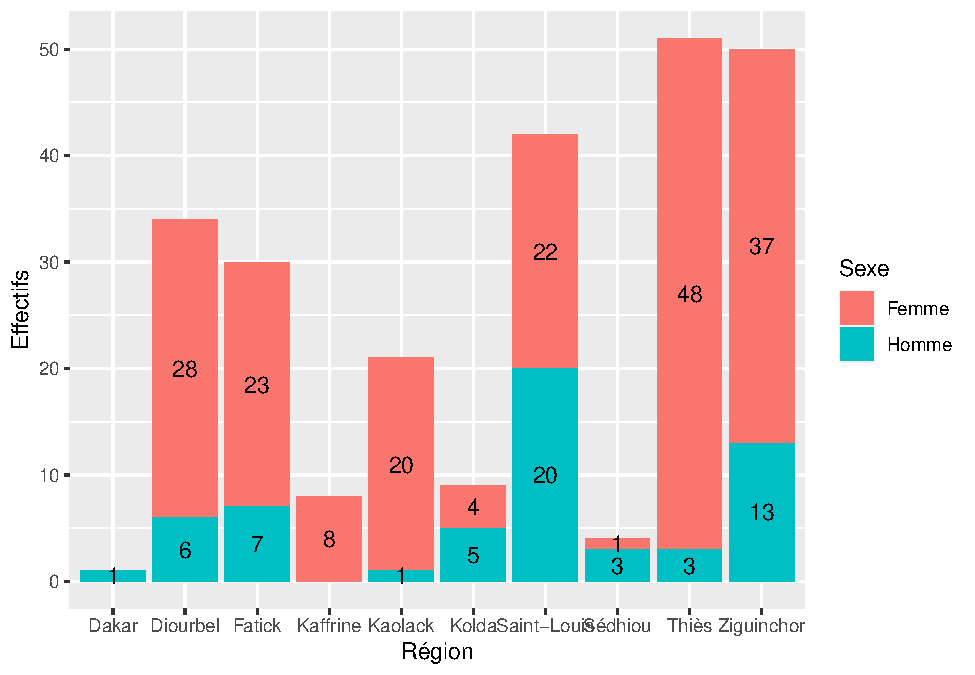
\includegraphics{RMarkdown_files/figure-latex/unnamed-chunk-15-1.pdf}

\begin{itemize}
\tightlist
\item
  \textbf{Distribution de la population suivant la langue parlée(Fraçais
  et wolof):}
\end{itemize}

\begin{Shaded}
\begin{Highlighting}[]
\NormalTok{data }\OtherTok{\textless{}{-}}\NormalTok{ projet }\SpecialCharTok{\%\textgreater{}\%} 
  \FunctionTok{rename}\NormalTok{(}\AttributeTok{Niveau\_instruction =}\NormalTok{ q25, }\AttributeTok{Propriete =}\NormalTok{ q81)}
\NormalTok{data }\OtherTok{\textless{}{-}}\NormalTok{ data }\SpecialCharTok{\%\textgreater{}\%}
  \FunctionTok{mutate}\NormalTok{(parle\_français }\OtherTok{=} \FunctionTok{ifelse}\NormalTok{(q24a\_1 }\SpecialCharTok{==} \DecValTok{1}\NormalTok{, }\StringTok{"Oui"}\NormalTok{, }\StringTok{"Non"}\NormalTok{),}
         \AttributeTok{parle\_wolof =} \FunctionTok{ifelse}\NormalTok{(q24a\_2 }\SpecialCharTok{==} \DecValTok{1}\NormalTok{, }\StringTok{"Oui"}\NormalTok{, }\StringTok{"Non"}\NormalTok{))}
\FunctionTok{ggbivariate}\NormalTok{(}\AttributeTok{data =}\NormalTok{ data , }\AttributeTok{outcome =} \StringTok{"parle\_wolof"}\NormalTok{, }\AttributeTok{explanatory =} \FunctionTok{c}\NormalTok{(}\StringTok{"sexe"}\NormalTok{, }\StringTok{"region"}\NormalTok{, }\StringTok{"Niveau\_instruction"}\NormalTok{, }\StringTok{"Propriete"}\NormalTok{))}
\end{Highlighting}
\end{Shaded}

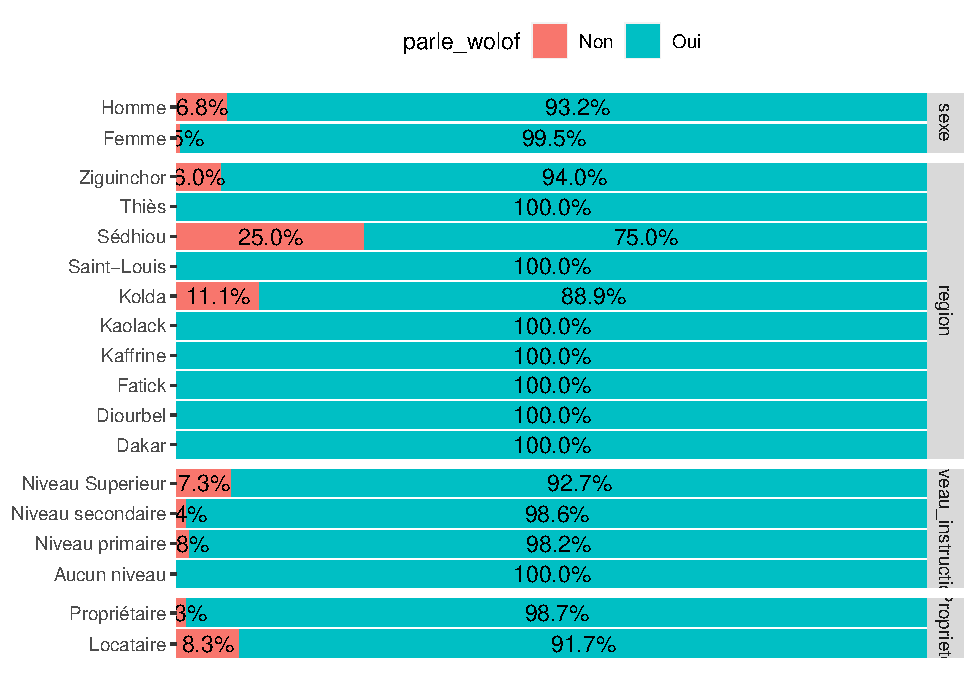
\includegraphics{RMarkdown_files/figure-latex/unnamed-chunk-16-1.pdf}

\begin{Shaded}
\begin{Highlighting}[]
\FunctionTok{ggbivariate}\NormalTok{(}\AttributeTok{data =}\NormalTok{ data , }\AttributeTok{outcome =} \StringTok{"parle\_français"}\NormalTok{, }\AttributeTok{explanatory =} \FunctionTok{c}\NormalTok{(}\StringTok{"sexe"}\NormalTok{, }\StringTok{"region"}\NormalTok{, }\StringTok{"Niveau\_instruction"}\NormalTok{, }\StringTok{"Propriete"}\NormalTok{))}
\end{Highlighting}
\end{Shaded}

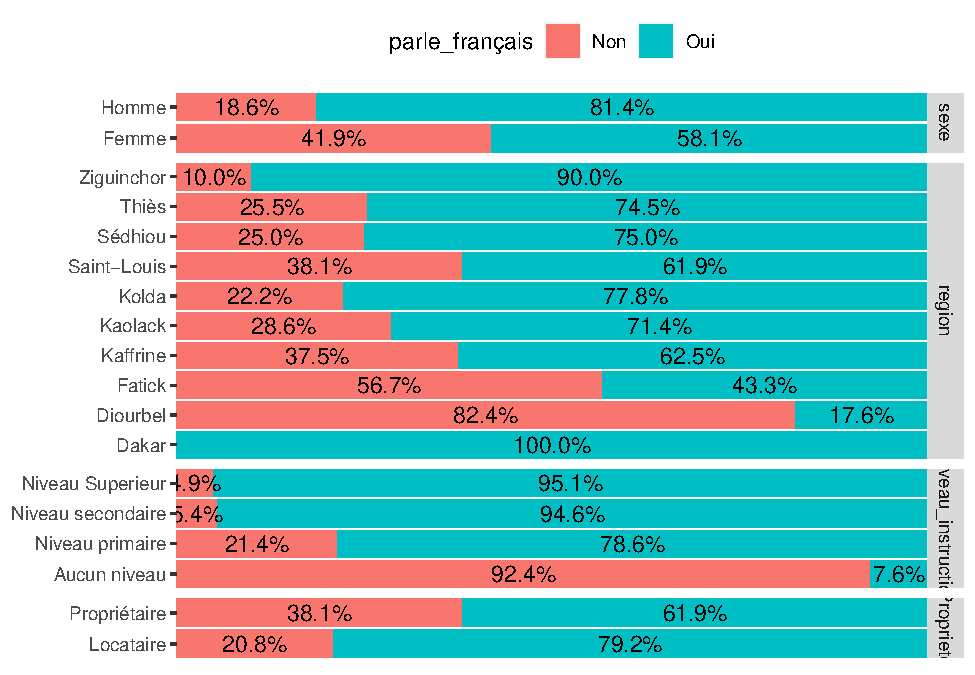
\includegraphics{RMarkdown_files/figure-latex/unnamed-chunk-16-2.pdf}

\hypertarget{cartographie}{%
\subsection{Cartographie}\label{cartographie}}

\begin{itemize}
\tightlist
\item
  Transformation du data.frame en données géographiques dont l'objet est
  nommé projet\_map :
\end{itemize}

\begin{Shaded}
\begin{Highlighting}[]
\CommentTok{\# Chargement des données de la carte du Sénégal}
\CommentTok{\# Nous lisons le fichier contenant la carte du Sénégal et le stockons }
\CommentTok{\# dans la variable "senegal"}
\NormalTok{senegal }\OtherTok{=} \FunctionTok{st\_read}\NormalTok{(}\StringTok{"Bases/gadm41\_SEN\_shp/gadm41\_SEN\_1.shp"}\NormalTok{)}
\end{Highlighting}
\end{Shaded}

\begin{verbatim}
## Reading layer `gadm41_SEN_1' from data source 
##   `D:\Mon phone\ISE\1ère année\S2\Projet sur R\Projet_R_ENSAE_2023\Bases\gadm41_SEN_shp\gadm41_SEN_1.shp' 
##   using driver `ESRI Shapefile'
## Simple feature collection with 14 features and 11 fields
## Geometry type: MULTIPOLYGON
## Dimension:     XY
## Bounding box:  xmin: -17.54319 ymin: 12.30786 xmax: -11.34247 ymax: 16.69207
## Geodetic CRS:  WGS 84
\end{verbatim}

\begin{Shaded}
\begin{Highlighting}[]
\CommentTok{\# La fonction st\_as\_sf convertit l\textquotesingle{}objet "projet" en objet }
\CommentTok{\# sf (spatial feature) en spécifiant les coordonnées GPS à utiliser}
\NormalTok{projet\_map }\OtherTok{=} \FunctionTok{st\_as\_sf}\NormalTok{(projet, }\AttributeTok{coords =} \FunctionTok{c}\NormalTok{(}\StringTok{"gps\_menlongitude"}\NormalTok{, }\StringTok{"gps\_menlatitude"}\NormalTok{), }\AttributeTok{crs=}\FunctionTok{st\_crs}\NormalTok{(senegal), }\AttributeTok{agr =} \StringTok{"constant"}\NormalTok{)}

\CommentTok{\# Jointure des données du projet avec la carte du Sénégal}
\NormalTok{projet\_map }\OtherTok{=} \FunctionTok{st\_join}\NormalTok{(projet\_map, senegal)}
\end{Highlighting}
\end{Shaded}

\begin{itemize}
\tightlist
\item
  Représentation spatiale des PME suivant le sexe:
\end{itemize}

\begin{Shaded}
\begin{Highlighting}[]
\CommentTok{\# Création de la première carte avec la répartition des PME suivant le sexe}
\FunctionTok{ggplot}\NormalTok{() }\SpecialCharTok{+}
  \FunctionTok{geom\_sf}\NormalTok{(}\AttributeTok{data=}\NormalTok{senegal)}\SpecialCharTok{+}
  \FunctionTok{geom\_sf\_text}\NormalTok{(}\AttributeTok{data=}\NormalTok{senegal, }\FunctionTok{aes}\NormalTok{(}\AttributeTok{label=}\NormalTok{NAME\_1))}\SpecialCharTok{+}
  \FunctionTok{geom\_sf}\NormalTok{(}\AttributeTok{data=}\NormalTok{projet\_map, }\FunctionTok{aes}\NormalTok{(}\AttributeTok{color=}\NormalTok{sexe), }\AttributeTok{size=}\DecValTok{2}\NormalTok{)}\SpecialCharTok{+}
  \FunctionTok{scale\_color\_manual}\NormalTok{(}\AttributeTok{values=}\FunctionTok{c}\NormalTok{(}\StringTok{"blue"}\NormalTok{, }\StringTok{"red"}\NormalTok{))}\SpecialCharTok{+}
  \FunctionTok{labs}\NormalTok{(}\AttributeTok{title =} \StringTok{"Répartition des PME suivant le sexe"}\NormalTok{,}
       \AttributeTok{subtitle =} \StringTok{"Carte du Sénégal"}\NormalTok{,}
       \AttributeTok{color =} \StringTok{"Sexe"}\NormalTok{) }\SpecialCharTok{+}
  \FunctionTok{theme\_minimal}\NormalTok{() }\SpecialCharTok{+}
  \FunctionTok{theme}\NormalTok{(}
    \AttributeTok{plot.title =} \FunctionTok{element\_text}\NormalTok{(}\AttributeTok{hjust =} \FloatTok{0.5}\NormalTok{, }\AttributeTok{face =} \StringTok{"bold"}\NormalTok{),}
    \AttributeTok{plot.subtitle =} \FunctionTok{element\_text}\NormalTok{(}\AttributeTok{hjust =} \FloatTok{0.5}\NormalTok{, }\AttributeTok{face =} \StringTok{"bold"}\NormalTok{))}\SpecialCharTok{+}
  \FunctionTok{coord\_sf}\NormalTok{(}\AttributeTok{datum =} \ConstantTok{NA}\NormalTok{)}\SpecialCharTok{+}
  \FunctionTok{annotation\_scale}\NormalTok{(}\AttributeTok{location =} \StringTok{"bl"}\NormalTok{, }\AttributeTok{text\_col =} \StringTok{"black"}\NormalTok{)}\SpecialCharTok{+}
  \FunctionTok{annotation\_north\_arrow}\NormalTok{(}\AttributeTok{location =} \StringTok{"tl"}\NormalTok{)}
\end{Highlighting}
\end{Shaded}

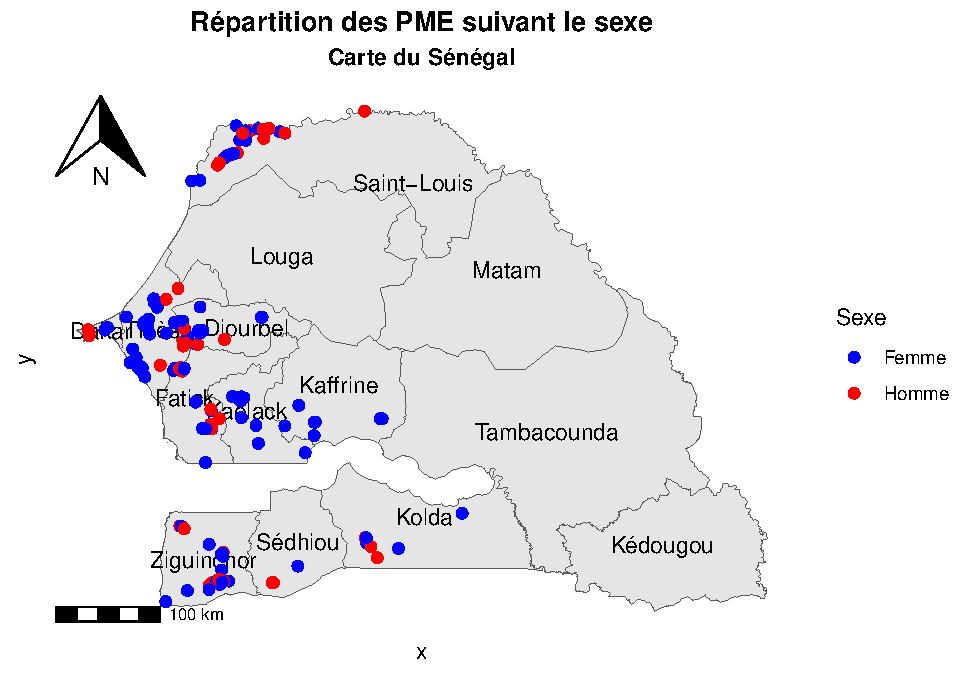
\includegraphics{RMarkdown_files/figure-latex/unnamed-chunk-18-1.pdf}

\begin{itemize}
\tightlist
\item
  Représentation spatiale des PME suivant le niveau d'instruction:
\end{itemize}

\begin{Shaded}
\begin{Highlighting}[]
\CommentTok{\# Renommons la variable q25 en Niveau\_instruction}
\NormalTok{projet\_map }\OtherTok{\textless{}{-}}\NormalTok{ projet\_map }\SpecialCharTok{\%\textgreater{}\%} \FunctionTok{rename}\NormalTok{(}\AttributeTok{Niveau\_instruction =}\NormalTok{ q25)}

\CommentTok{\# Création de la deuxième carte avec la répartition des PME  }
\CommentTok{\# suivant le niveau d\textquotesingle{}instruction}
\FunctionTok{ggplot}\NormalTok{() }\SpecialCharTok{+}
  \FunctionTok{geom\_sf}\NormalTok{(}\AttributeTok{data=}\NormalTok{senegal)}\SpecialCharTok{+}
  \FunctionTok{geom\_sf\_text}\NormalTok{(}\AttributeTok{data=}\NormalTok{senegal, }\FunctionTok{aes}\NormalTok{(}\AttributeTok{label=}\NormalTok{NAME\_1))}\SpecialCharTok{+}
  \FunctionTok{geom\_sf}\NormalTok{(}\AttributeTok{data =}\NormalTok{ projet\_map, }\FunctionTok{aes}\NormalTok{(}\AttributeTok{color =}\NormalTok{ Niveau\_instruction), }\AttributeTok{size =}\DecValTok{3}\NormalTok{) }\SpecialCharTok{+}
  \FunctionTok{scale\_color\_manual}\NormalTok{(}\AttributeTok{values=}\FunctionTok{c}\NormalTok{(}\StringTok{"red"}\NormalTok{, }\StringTok{"blue"}\NormalTok{, }\StringTok{"green"}\NormalTok{, }\StringTok{"yellow"}\NormalTok{)) }\SpecialCharTok{+}
  \FunctionTok{labs}\NormalTok{(}\AttributeTok{title =} \StringTok{"Répartition des PME suivant le niveau d\textquotesingle{}instruction"}\NormalTok{,}
       \AttributeTok{subtitle =} \StringTok{"Carte du Sénégal"}\NormalTok{) }\SpecialCharTok{+}
  \FunctionTok{theme\_minimal}\NormalTok{() }\SpecialCharTok{+}
  \FunctionTok{theme}\NormalTok{(}
    \AttributeTok{plot.title =} \FunctionTok{element\_text}\NormalTok{(}\AttributeTok{hjust =} \FloatTok{0.5}\NormalTok{, }\AttributeTok{face =} \StringTok{"bold"}\NormalTok{),}
    \AttributeTok{plot.subtitle =} \FunctionTok{element\_text}\NormalTok{(}\AttributeTok{hjust =} \FloatTok{0.5}\NormalTok{, }\AttributeTok{face =} \StringTok{"bold"}\NormalTok{))}\SpecialCharTok{+}
  \FunctionTok{coord\_sf}\NormalTok{(}\AttributeTok{datum =} \ConstantTok{NA}\NormalTok{)}\SpecialCharTok{+}
  \FunctionTok{annotation\_scale}\NormalTok{(}\AttributeTok{location =} \StringTok{"bl"}\NormalTok{, }\AttributeTok{text\_col =} \StringTok{"black"}\NormalTok{)}\SpecialCharTok{+}
  \FunctionTok{annotation\_north\_arrow}\NormalTok{(}\AttributeTok{location =} \StringTok{"tl"}\NormalTok{)}
\end{Highlighting}
\end{Shaded}

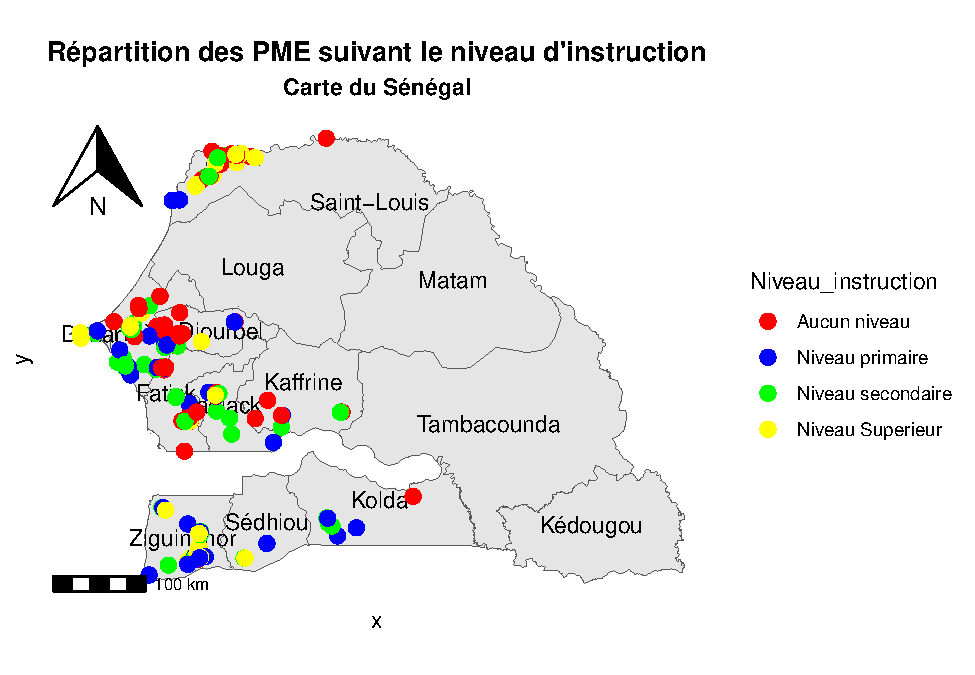
\includegraphics{RMarkdown_files/figure-latex/unnamed-chunk-19-1.pdf}

\begin{itemize}
\tightlist
\item
  Analyse spatiale de notre choix
\end{itemize}

\begin{Shaded}
\begin{Highlighting}[]
\CommentTok{\# Création de la troisième carte avec la répartition des PME suivant prop}

\CommentTok{\# Renommons la variable q81 en Propriéte}
\NormalTok{projet\_map }\OtherTok{\textless{}{-}}\NormalTok{ projet\_map }\SpecialCharTok{\%\textgreater{}\%} \FunctionTok{rename}\NormalTok{(}\AttributeTok{Propriete =}\NormalTok{ q81)}
\FunctionTok{ggplot}\NormalTok{() }\SpecialCharTok{+}
  \FunctionTok{geom\_sf}\NormalTok{(}\AttributeTok{data=}\NormalTok{senegal)}\SpecialCharTok{+}
  \FunctionTok{geom\_sf\_text}\NormalTok{(}\AttributeTok{data=}\NormalTok{senegal, }\FunctionTok{aes}\NormalTok{(}\AttributeTok{label=}\NormalTok{NAME\_1))}\SpecialCharTok{+}
  \FunctionTok{geom\_sf}\NormalTok{(}\AttributeTok{data=}\NormalTok{projet\_map, }\FunctionTok{aes}\NormalTok{(}\AttributeTok{color=}\NormalTok{Propriete), }\AttributeTok{size=}\DecValTok{2}\NormalTok{)}\SpecialCharTok{+}
  \FunctionTok{scale\_color\_manual}\NormalTok{(}\AttributeTok{values=}\FunctionTok{c}\NormalTok{(}\StringTok{"blue"}\NormalTok{, }\StringTok{"red"}\NormalTok{))}\SpecialCharTok{+}
  \FunctionTok{labs}\NormalTok{(}\AttributeTok{title =} \StringTok{"Répartition des PME suivant la propriété"}\NormalTok{,}
       \AttributeTok{subtitle =} \StringTok{"Carte du Sénégal"}\NormalTok{) }\SpecialCharTok{+}
  \FunctionTok{theme\_minimal}\NormalTok{() }\SpecialCharTok{+}
  \FunctionTok{theme}\NormalTok{(}
    \AttributeTok{plot.title =} \FunctionTok{element\_text}\NormalTok{(}\AttributeTok{hjust =} \FloatTok{0.5}\NormalTok{, }\AttributeTok{face =} \StringTok{"bold"}\NormalTok{),}
    \AttributeTok{plot.subtitle =} \FunctionTok{element\_text}\NormalTok{(}\AttributeTok{hjust =} \FloatTok{0.5}\NormalTok{, }\AttributeTok{face =} \StringTok{"bold"}\NormalTok{))}\SpecialCharTok{+}
  \FunctionTok{coord\_sf}\NormalTok{(}\AttributeTok{datum =} \ConstantTok{NA}\NormalTok{)}\SpecialCharTok{+}
  \FunctionTok{annotation\_scale}\NormalTok{(}\AttributeTok{location =} \StringTok{"bl"}\NormalTok{, }\AttributeTok{text\_col =} \StringTok{"black"}\NormalTok{)}\SpecialCharTok{+}
  \FunctionTok{annotation\_north\_arrow}\NormalTok{(}\AttributeTok{location =} \StringTok{"tl"}\NormalTok{)}
\end{Highlighting}
\end{Shaded}

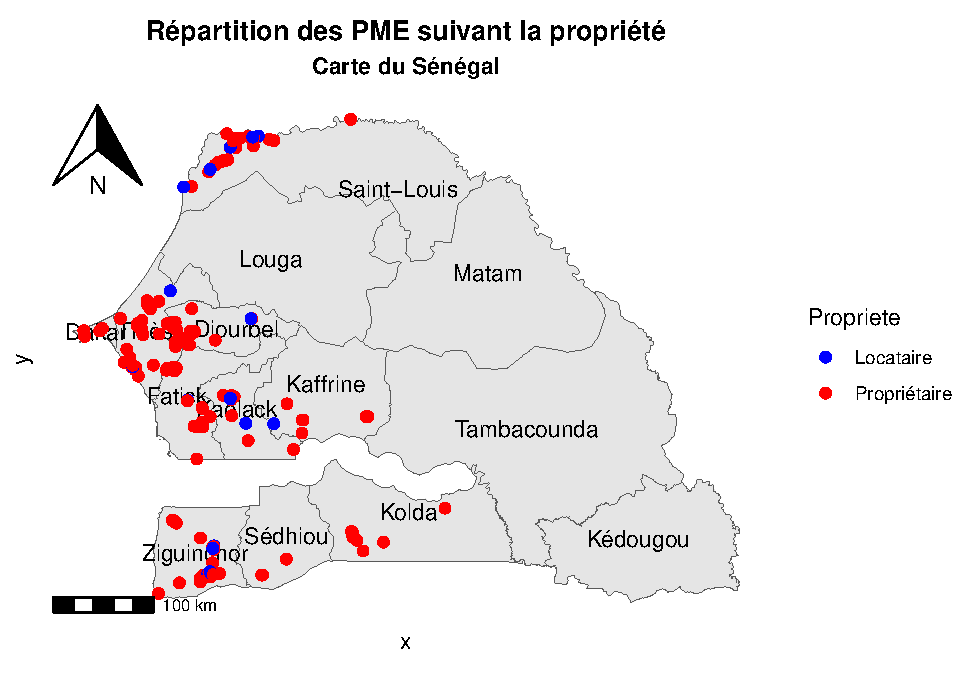
\includegraphics{RMarkdown_files/figure-latex/unnamed-chunk-20-1.pdf}

\hypertarget{partie-2}{%
\section{Partie 2}\label{partie-2}}

\hypertarget{nettoyage-et-gestion-des-donnuxe9es}{%
\subsection{Nettoyage et gestion des
données}\label{nettoyage-et-gestion-des-donnuxe9es}}

\begin{itemize}
\tightlist
\item
  Chargement des données et effectuons le nettoyage initial
\end{itemize}

\begin{Shaded}
\begin{Highlighting}[]
\CommentTok{\# Chargement les données}
\NormalTok{feuille1 }\OtherTok{\textless{}{-}} \FunctionTok{read\_excel}\NormalTok{(}\StringTok{"Bases/Base\_Partie 2.xlsx"}\NormalTok{, }\AttributeTok{sheet =} \DecValTok{1}\NormalTok{)}

\CommentTok{\# Renommons la variable "country\_destination" en "destination" et }
\CommentTok{\# définissons les valeurs négatives comme manquantes}
\NormalTok{feuille1 }\OtherTok{\textless{}{-}}\NormalTok{ feuille1 }\SpecialCharTok{\%\textgreater{}\%}
  \FunctionTok{rename}\NormalTok{(}\AttributeTok{destination =}\NormalTok{ country\_destination) }\SpecialCharTok{\%\textgreater{}\%}
  \FunctionTok{mutate}\NormalTok{(}\AttributeTok{destination =} \FunctionTok{ifelse}\NormalTok{(destination }\SpecialCharTok{\textless{}} \DecValTok{0}\NormalTok{, }\ConstantTok{NA}\NormalTok{, destination))}
\end{Highlighting}
\end{Shaded}

\begin{itemize}
\tightlist
\item
  Création d'une nouvelle variable contenant des tranches d'âge de 5 ans
\end{itemize}

\begin{Shaded}
\begin{Highlighting}[]
\CommentTok{\# Imputons la valeur abérante par la médiane}

\CommentTok{\# Calculer la médiane des valeurs non aberrantes (différentes de 999) dans la variable "age" et remplacer les valeurs 999 par la médiane}
\NormalTok{feuille1 }\OtherTok{\textless{}{-}}\NormalTok{ feuille1 }\SpecialCharTok{\%\textgreater{}\%}
  \FunctionTok{mutate}\NormalTok{(}\AttributeTok{age =} \FunctionTok{replace}\NormalTok{(age, age }\SpecialCharTok{==} \DecValTok{999}\NormalTok{, }\FunctionTok{median}\NormalTok{(age[age }\SpecialCharTok{!=} \DecValTok{999}\NormalTok{], }\AttributeTok{na.rm =} \ConstantTok{TRUE}\NormalTok{)))}


\CommentTok{\# Créons la variable tranche\_age contenant des tranches d\textquotesingle{}âge de}
\CommentTok{\# 5 ans}
\NormalTok{feuille1 }\OtherTok{\textless{}{-}}\NormalTok{ feuille1 }\SpecialCharTok{\%\textgreater{}\%}
  \FunctionTok{mutate}\NormalTok{(}\AttributeTok{tranche\_age =} \FunctionTok{cut}\NormalTok{(age, }\AttributeTok{breaks =} \FunctionTok{seq}\NormalTok{(}\DecValTok{0}\NormalTok{, }\FunctionTok{max}\NormalTok{(age), }\AttributeTok{by =} \DecValTok{5}\NormalTok{), }\AttributeTok{include.lowest =} \ConstantTok{TRUE}\NormalTok{))}
\end{Highlighting}
\end{Shaded}

\begin{itemize}
\tightlist
\item
  Création d'une nouvelle variable contenant le nombre d'entretiens
  réalisés par chaque agent recenseur :
\end{itemize}

\begin{Shaded}
\begin{Highlighting}[]
\NormalTok{feuille1 }\OtherTok{\textless{}{-}}\NormalTok{ feuille1 }\SpecialCharTok{\%\textgreater{}\%}
  \FunctionTok{group\_by}\NormalTok{(enumerator) }\SpecialCharTok{\%\textgreater{}\%}
  \FunctionTok{mutate}\NormalTok{(}\AttributeTok{nombre\_entretiens =} \FunctionTok{n}\NormalTok{()) }\SpecialCharTok{\%\textgreater{}\%}
  \FunctionTok{ungroup}\NormalTok{()}
\end{Highlighting}
\end{Shaded}

\begin{itemize}
\tightlist
\item
  Création d'une nouvelle variable qui affecte aléatoirement chaque
  répondant à un groupe de traitement (1) ou de contrôle (0)
\end{itemize}

\begin{Shaded}
\begin{Highlighting}[]
\NormalTok{feuille1 }\OtherTok{\textless{}{-}}\NormalTok{ feuille1 }\SpecialCharTok{\%\textgreater{}\%}
  \FunctionTok{mutate}\NormalTok{(}\AttributeTok{groupe =}\NormalTok{ \{}\FunctionTok{set.seed}\NormalTok{(}\DecValTok{123}\NormalTok{); }\FunctionTok{sample}\NormalTok{(}\FunctionTok{c}\NormalTok{(}\DecValTok{0}\NormalTok{, }\DecValTok{1}\NormalTok{), }\AttributeTok{size =} \FunctionTok{n}\NormalTok{(), }\AttributeTok{replace =} \ConstantTok{TRUE}\NormalTok{)\})}
\end{Highlighting}
\end{Shaded}

\begin{itemize}
\tightlist
\item
  Fusion de la taille de la population de chaque district (feuille 2)
  avec l'ensemble de données (feuille 1) :
\end{itemize}

\begin{Shaded}
\begin{Highlighting}[]
\CommentTok{\# Charger les données de la deuxième feuille}
\NormalTok{feuille2 }\OtherTok{\textless{}{-}} \FunctionTok{read\_excel}\NormalTok{(}\StringTok{"Bases/Base\_Partie 2.xlsx"}\NormalTok{, }\AttributeTok{sheet =} \DecValTok{2}\NormalTok{)}

\CommentTok{\# Fusion}
\NormalTok{feuille1 }\OtherTok{\textless{}{-}}\NormalTok{ feuille1 }\SpecialCharTok{\%\textgreater{}\%}
  \FunctionTok{left\_join}\NormalTok{(feuille2, }\AttributeTok{by =} \StringTok{"district"}\NormalTok{)}
\end{Highlighting}
\end{Shaded}

\begin{itemize}
\tightlist
\item
  Calcul la durée de l'entretien et indiquer la durée moyenne de
  l'entretien par enquêteur :
\end{itemize}

\begin{Shaded}
\begin{Highlighting}[]
\NormalTok{feuille1 }\OtherTok{\textless{}{-}}\NormalTok{ feuille1 }\SpecialCharTok{\%\textgreater{}\%}
  \FunctionTok{mutate}\NormalTok{(}\AttributeTok{duree\_entretien =}\NormalTok{ endtime }\SpecialCharTok{{-}}\NormalTok{ starttime) }\SpecialCharTok{\%\textgreater{}\%}
  \FunctionTok{group\_by}\NormalTok{(enumerator) }\SpecialCharTok{\%\textgreater{}\%}
  \FunctionTok{mutate}\NormalTok{(}\AttributeTok{duree\_moyenne\_entretien =} \FunctionTok{mean}\NormalTok{(duree\_entretien)) }\SpecialCharTok{\%\textgreater{}\%}
  \FunctionTok{ungroup}\NormalTok{()}
\end{Highlighting}
\end{Shaded}

\begin{itemize}
\tightlist
\item
  Renommage de toutes les variables de l'ensemble de données en ajoutant
  le préfixe ``endline\_'' à l'aide d'une boucle :
\end{itemize}

\begin{Shaded}
\begin{Highlighting}[]
\NormalTok{copie }\OtherTok{=}\NormalTok{ feuille1}
\NormalTok{feuille1 }\OtherTok{\textless{}{-}}\NormalTok{ feuille1 }\SpecialCharTok{\%\textgreater{}\%}
  \FunctionTok{rename\_all}\NormalTok{(}\SpecialCharTok{\textasciitilde{}}\FunctionTok{paste0}\NormalTok{(}\StringTok{"endline\_"}\NormalTok{, .))}
\end{Highlighting}
\end{Shaded}

\hypertarget{analyse-et-visualisation-des-donnuxe9es}{%
\subsection{Analyse et visualisation des
données}\label{analyse-et-visualisation-des-donnuxe9es}}

\begin{itemize}
\tightlist
\item
  Création d'un tableau récapitulatif contenant l'âge moyen et le nombre
  moyen d'enfants par district :
\end{itemize}

\begin{Shaded}
\begin{Highlighting}[]
\NormalTok{feuille1 }\SpecialCharTok{\%\textgreater{}\%}
  \FunctionTok{tbl\_summary}\NormalTok{(}
    \AttributeTok{by =}\NormalTok{ endline\_district,}
    \AttributeTok{include =} \FunctionTok{c}\NormalTok{(}\StringTok{"endline\_age"}\NormalTok{, }\StringTok{"endline\_children\_num"}\NormalTok{), }
    \AttributeTok{type =} \FunctionTok{list}\NormalTok{(}\AttributeTok{endline\_children\_num =} \StringTok{"continuous"}\NormalTok{),}
    \AttributeTok{statistic =} \FunctionTok{all\_continuous}\NormalTok{() }\SpecialCharTok{\textasciitilde{}} \StringTok{"\{mean\}"}\NormalTok{,}
    \AttributeTok{label=}\FunctionTok{list}\NormalTok{( endline\_age}\SpecialCharTok{\textasciitilde{}} \StringTok{"Age moyen"}\NormalTok{, }
\NormalTok{                endline\_children\_num }\SpecialCharTok{\textasciitilde{}} \StringTok{"Nombre moyen d\textquotesingle{}enfants"}\NormalTok{)}
\NormalTok{    ) }\SpecialCharTok{\%\textgreater{}\%}
  \FunctionTok{add\_overall}\NormalTok{() }\SpecialCharTok{\%\textgreater{}\%}
  \FunctionTok{modify\_header}\NormalTok{(label }\SpecialCharTok{\textasciitilde{}} \StringTok{""}\NormalTok{) }\SpecialCharTok{\%\textgreater{}\%}
  \FunctionTok{modify\_spanning\_header}\NormalTok{(}\FunctionTok{all\_stat\_cols}\NormalTok{() }\SpecialCharTok{\textasciitilde{}} \StringTok{"**District**"}\NormalTok{) }\SpecialCharTok{\%\textgreater{}\%}
  \FunctionTok{bold\_labels}\NormalTok{() }\SpecialCharTok{\%\textgreater{}\%}
  \FunctionTok{as\_flex\_table}\NormalTok{() }\SpecialCharTok{\%\textgreater{}\%}
  \FunctionTok{fontsize}\NormalTok{(}\AttributeTok{size =} \DecValTok{10}\NormalTok{) }\SpecialCharTok{\%\textgreater{}\%}
  \FunctionTok{width}\NormalTok{(}\AttributeTok{width =} \FloatTok{0.6}\NormalTok{)}
\end{Highlighting}
\end{Shaded}

\global\setlength{\Oldarrayrulewidth}{\arrayrulewidth}

\global\setlength{\Oldtabcolsep}{\tabcolsep}

\setlength{\tabcolsep}{0pt}

\renewcommand*{\arraystretch}{1.5}



\providecommand{\ascline}[3]{\noalign{\global\arrayrulewidth #1}\arrayrulecolor[HTML]{#2}\cline{#3}}

\begin{longtable}[c]{|p{0.60in}|p{0.60in}|p{0.60in}|p{0.60in}|p{0.60in}|p{0.60in}|p{0.60in}|p{0.60in}|p{0.60in}|p{0.60in}}



\ascline{1pt}{000000}{1-10}

\multicolumn{1}{>{\raggedright}m{\dimexpr 0.6in+0\tabcolsep}}{\textcolor[HTML]{000000}{\fontsize{11}{11}\selectfont{\ }}} & \multicolumn{9}{>{\centering}m{\dimexpr 5.4in+16\tabcolsep}}{\textcolor[HTML]{000000}{\fontsize{11}{11}\selectfont{\textbf{District}}}} \\

\ascline{1pt}{000000}{1-10}



\multicolumn{1}{>{\raggedright}m{\dimexpr 0.6in+0\tabcolsep}}{\textcolor[HTML]{000000}{\fontsize{11}{11}\selectfont{}}} & \multicolumn{1}{>{\centering}m{\dimexpr 0.6in+0\tabcolsep}}{\textcolor[HTML]{000000}{\fontsize{11}{11}\selectfont{\textbf{Overall}}}\textcolor[HTML]{000000}{\fontsize{11}{11}\selectfont{,\ N\ =\ 97}}\textcolor[HTML]{000000}{\textsuperscript{\fontsize{11}{11}\selectfont{1}}}} & \multicolumn{1}{>{\centering}m{\dimexpr 0.6in+0\tabcolsep}}{\textcolor[HTML]{000000}{\fontsize{11}{11}\selectfont{\textbf{1}}}\textcolor[HTML]{000000}{\fontsize{11}{11}\selectfont{,\ N\ =\ 8}}\textcolor[HTML]{000000}{\textsuperscript{\fontsize{11}{11}\selectfont{1}}}} & \multicolumn{1}{>{\centering}m{\dimexpr 0.6in+0\tabcolsep}}{\textcolor[HTML]{000000}{\fontsize{11}{11}\selectfont{\textbf{2}}}\textcolor[HTML]{000000}{\fontsize{11}{11}\selectfont{,\ N\ =\ 27}}\textcolor[HTML]{000000}{\textsuperscript{\fontsize{11}{11}\selectfont{1}}}} & \multicolumn{1}{>{\centering}m{\dimexpr 0.6in+0\tabcolsep}}{\textcolor[HTML]{000000}{\fontsize{11}{11}\selectfont{\textbf{3}}}\textcolor[HTML]{000000}{\fontsize{11}{11}\selectfont{,\ N\ =\ 8}}\textcolor[HTML]{000000}{\textsuperscript{\fontsize{11}{11}\selectfont{1}}}} & \multicolumn{1}{>{\centering}m{\dimexpr 0.6in+0\tabcolsep}}{\textcolor[HTML]{000000}{\fontsize{11}{11}\selectfont{\textbf{4}}}\textcolor[HTML]{000000}{\fontsize{11}{11}\selectfont{,\ N\ =\ 5}}\textcolor[HTML]{000000}{\textsuperscript{\fontsize{11}{11}\selectfont{1}}}} & \multicolumn{1}{>{\centering}m{\dimexpr 0.6in+0\tabcolsep}}{\textcolor[HTML]{000000}{\fontsize{11}{11}\selectfont{\textbf{5}}}\textcolor[HTML]{000000}{\fontsize{11}{11}\selectfont{,\ N\ =\ 6}}\textcolor[HTML]{000000}{\textsuperscript{\fontsize{11}{11}\selectfont{1}}}} & \multicolumn{1}{>{\centering}m{\dimexpr 0.6in+0\tabcolsep}}{\textcolor[HTML]{000000}{\fontsize{11}{11}\selectfont{\textbf{6}}}\textcolor[HTML]{000000}{\fontsize{11}{11}\selectfont{,\ N\ =\ 26}}\textcolor[HTML]{000000}{\textsuperscript{\fontsize{11}{11}\selectfont{1}}}} & \multicolumn{1}{>{\centering}m{\dimexpr 0.6in+0\tabcolsep}}{\textcolor[HTML]{000000}{\fontsize{11}{11}\selectfont{\textbf{7}}}\textcolor[HTML]{000000}{\fontsize{11}{11}\selectfont{,\ N\ =\ 6}}\textcolor[HTML]{000000}{\textsuperscript{\fontsize{11}{11}\selectfont{1}}}} & \multicolumn{1}{>{\centering}m{\dimexpr 0.6in+0\tabcolsep}}{\textcolor[HTML]{000000}{\fontsize{11}{11}\selectfont{\textbf{8}}}\textcolor[HTML]{000000}{\fontsize{11}{11}\selectfont{,\ N\ =\ 11}}\textcolor[HTML]{000000}{\textsuperscript{\fontsize{11}{11}\selectfont{1}}}} \\

\ascline{1pt}{000000}{1-10}\endfirsthead 

\ascline{1pt}{000000}{1-10}

\multicolumn{1}{>{\raggedright}m{\dimexpr 0.6in+0\tabcolsep}}{\textcolor[HTML]{000000}{\fontsize{11}{11}\selectfont{\ }}} & \multicolumn{9}{>{\centering}m{\dimexpr 5.4in+16\tabcolsep}}{\textcolor[HTML]{000000}{\fontsize{11}{11}\selectfont{\textbf{District}}}} \\

\ascline{1pt}{000000}{1-10}



\multicolumn{1}{>{\raggedright}m{\dimexpr 0.6in+0\tabcolsep}}{\textcolor[HTML]{000000}{\fontsize{11}{11}\selectfont{}}} & \multicolumn{1}{>{\centering}m{\dimexpr 0.6in+0\tabcolsep}}{\textcolor[HTML]{000000}{\fontsize{11}{11}\selectfont{\textbf{Overall}}}\textcolor[HTML]{000000}{\fontsize{11}{11}\selectfont{,\ N\ =\ 97}}\textcolor[HTML]{000000}{\textsuperscript{\fontsize{11}{11}\selectfont{1}}}} & \multicolumn{1}{>{\centering}m{\dimexpr 0.6in+0\tabcolsep}}{\textcolor[HTML]{000000}{\fontsize{11}{11}\selectfont{\textbf{1}}}\textcolor[HTML]{000000}{\fontsize{11}{11}\selectfont{,\ N\ =\ 8}}\textcolor[HTML]{000000}{\textsuperscript{\fontsize{11}{11}\selectfont{1}}}} & \multicolumn{1}{>{\centering}m{\dimexpr 0.6in+0\tabcolsep}}{\textcolor[HTML]{000000}{\fontsize{11}{11}\selectfont{\textbf{2}}}\textcolor[HTML]{000000}{\fontsize{11}{11}\selectfont{,\ N\ =\ 27}}\textcolor[HTML]{000000}{\textsuperscript{\fontsize{11}{11}\selectfont{1}}}} & \multicolumn{1}{>{\centering}m{\dimexpr 0.6in+0\tabcolsep}}{\textcolor[HTML]{000000}{\fontsize{11}{11}\selectfont{\textbf{3}}}\textcolor[HTML]{000000}{\fontsize{11}{11}\selectfont{,\ N\ =\ 8}}\textcolor[HTML]{000000}{\textsuperscript{\fontsize{11}{11}\selectfont{1}}}} & \multicolumn{1}{>{\centering}m{\dimexpr 0.6in+0\tabcolsep}}{\textcolor[HTML]{000000}{\fontsize{11}{11}\selectfont{\textbf{4}}}\textcolor[HTML]{000000}{\fontsize{11}{11}\selectfont{,\ N\ =\ 5}}\textcolor[HTML]{000000}{\textsuperscript{\fontsize{11}{11}\selectfont{1}}}} & \multicolumn{1}{>{\centering}m{\dimexpr 0.6in+0\tabcolsep}}{\textcolor[HTML]{000000}{\fontsize{11}{11}\selectfont{\textbf{5}}}\textcolor[HTML]{000000}{\fontsize{11}{11}\selectfont{,\ N\ =\ 6}}\textcolor[HTML]{000000}{\textsuperscript{\fontsize{11}{11}\selectfont{1}}}} & \multicolumn{1}{>{\centering}m{\dimexpr 0.6in+0\tabcolsep}}{\textcolor[HTML]{000000}{\fontsize{11}{11}\selectfont{\textbf{6}}}\textcolor[HTML]{000000}{\fontsize{11}{11}\selectfont{,\ N\ =\ 26}}\textcolor[HTML]{000000}{\textsuperscript{\fontsize{11}{11}\selectfont{1}}}} & \multicolumn{1}{>{\centering}m{\dimexpr 0.6in+0\tabcolsep}}{\textcolor[HTML]{000000}{\fontsize{11}{11}\selectfont{\textbf{7}}}\textcolor[HTML]{000000}{\fontsize{11}{11}\selectfont{,\ N\ =\ 6}}\textcolor[HTML]{000000}{\textsuperscript{\fontsize{11}{11}\selectfont{1}}}} & \multicolumn{1}{>{\centering}m{\dimexpr 0.6in+0\tabcolsep}}{\textcolor[HTML]{000000}{\fontsize{11}{11}\selectfont{\textbf{8}}}\textcolor[HTML]{000000}{\fontsize{11}{11}\selectfont{,\ N\ =\ 11}}\textcolor[HTML]{000000}{\textsuperscript{\fontsize{11}{11}\selectfont{1}}}} \\

\ascline{1pt}{000000}{1-10}\endhead



\multicolumn{10}{>{\raggedright}m{\dimexpr 6in+18\tabcolsep}}{\textcolor[HTML]{000000}{\textsuperscript{\fontsize{11}{11}\selectfont{1}}}\textcolor[HTML]{000000}{\fontsize{11}{11}\selectfont{Mean}}} \\

\endfoot



\multicolumn{1}{>{\raggedright}p{\dimexpr 0.6in+0\tabcolsep}}{\textcolor[HTML]{000000}{\fontsize{10}{10}\selectfont{\textbf{Age\ moyen}}}} & \multicolumn{1}{>{\centering}p{\dimexpr 0.6in+0\tabcolsep}}{\textcolor[HTML]{000000}{\fontsize{10}{10}\selectfont{26}}} & \multicolumn{1}{>{\centering}p{\dimexpr 0.6in+0\tabcolsep}}{\textcolor[HTML]{000000}{\fontsize{10}{10}\selectfont{30}}} & \multicolumn{1}{>{\centering}p{\dimexpr 0.6in+0\tabcolsep}}{\textcolor[HTML]{000000}{\fontsize{10}{10}\selectfont{27}}} & \multicolumn{1}{>{\centering}p{\dimexpr 0.6in+0\tabcolsep}}{\textcolor[HTML]{000000}{\fontsize{10}{10}\selectfont{26}}} & \multicolumn{1}{>{\centering}p{\dimexpr 0.6in+0\tabcolsep}}{\textcolor[HTML]{000000}{\fontsize{10}{10}\selectfont{26}}} & \multicolumn{1}{>{\centering}p{\dimexpr 0.6in+0\tabcolsep}}{\textcolor[HTML]{000000}{\fontsize{10}{10}\selectfont{24}}} & \multicolumn{1}{>{\centering}p{\dimexpr 0.6in+0\tabcolsep}}{\textcolor[HTML]{000000}{\fontsize{10}{10}\selectfont{23}}} & \multicolumn{1}{>{\centering}p{\dimexpr 0.6in+0\tabcolsep}}{\textcolor[HTML]{000000}{\fontsize{10}{10}\selectfont{28}}} & \multicolumn{1}{>{\centering}p{\dimexpr 0.6in+0\tabcolsep}}{\textcolor[HTML]{000000}{\fontsize{10}{10}\selectfont{25}}} \\





\multicolumn{1}{>{\raggedright}p{\dimexpr 0.6in+0\tabcolsep}}{\textcolor[HTML]{000000}{\fontsize{10}{10}\selectfont{\textbf{Nombre\ moyen\ d'enfants}}}} & \multicolumn{1}{>{\centering}p{\dimexpr 0.6in+0\tabcolsep}}{\textcolor[HTML]{000000}{\fontsize{10}{10}\selectfont{0.58}}} & \multicolumn{1}{>{\centering}p{\dimexpr 0.6in+0\tabcolsep}}{\textcolor[HTML]{000000}{\fontsize{10}{10}\selectfont{1.50}}} & \multicolumn{1}{>{\centering}p{\dimexpr 0.6in+0\tabcolsep}}{\textcolor[HTML]{000000}{\fontsize{10}{10}\selectfont{0.85}}} & \multicolumn{1}{>{\centering}p{\dimexpr 0.6in+0\tabcolsep}}{\textcolor[HTML]{000000}{\fontsize{10}{10}\selectfont{0.00}}} & \multicolumn{1}{>{\centering}p{\dimexpr 0.6in+0\tabcolsep}}{\textcolor[HTML]{000000}{\fontsize{10}{10}\selectfont{0.00}}} & \multicolumn{1}{>{\centering}p{\dimexpr 0.6in+0\tabcolsep}}{\textcolor[HTML]{000000}{\fontsize{10}{10}\selectfont{0.50}}} & \multicolumn{1}{>{\centering}p{\dimexpr 0.6in+0\tabcolsep}}{\textcolor[HTML]{000000}{\fontsize{10}{10}\selectfont{0.12}}} & \multicolumn{1}{>{\centering}p{\dimexpr 0.6in+0\tabcolsep}}{\textcolor[HTML]{000000}{\fontsize{10}{10}\selectfont{0.17}}} & \multicolumn{1}{>{\centering}p{\dimexpr 0.6in+0\tabcolsep}}{\textcolor[HTML]{000000}{\fontsize{10}{10}\selectfont{1.27}}} \\

\ascline{1pt}{000000}{1-10}



\end{longtable}



\arrayrulecolor[HTML]{000000}

\global\setlength{\arrayrulewidth}{\Oldarrayrulewidth}

\global\setlength{\tabcolsep}{\Oldtabcolsep}

\renewcommand*{\arraystretch}{1}

\begin{itemize}
\tightlist
\item
  Testons si la différence d'âge entre les sexes est statistiquement
  significative au niveau de 5 \%:
\end{itemize}

\begin{Shaded}
\begin{Highlighting}[]
\DocumentationTok{\#\#\# différence d\textquotesingle{}âge entre les sexe}
\NormalTok{diff\_age }\OtherTok{\textless{}{-}}\NormalTok{ feuille1 }\SpecialCharTok{\%\textgreater{}\%} \FunctionTok{tbl\_summary}\NormalTok{(}
\AttributeTok{include =} \FunctionTok{c}\NormalTok{(endline\_age),}
\AttributeTok{by =}\NormalTok{ endline\_sex,}
\AttributeTok{statistic =} \SpecialCharTok{\textasciitilde{}}\StringTok{"\{mean\}"}\NormalTok{,}
\AttributeTok{label =} \FunctionTok{list}\NormalTok{(endline\_age }\SpecialCharTok{\textasciitilde{}} \StringTok{"Age du répondant"}\NormalTok{),}
\AttributeTok{digits =} \SpecialCharTok{\textasciitilde{}} \DecValTok{1}
\NormalTok{)}\SpecialCharTok{\%\textgreater{}\%} \FunctionTok{bold\_labels}\NormalTok{() }\SpecialCharTok{\%\textgreater{}\%} \FunctionTok{italicize\_levels}\NormalTok{() }\SpecialCharTok{\%\textgreater{}\%}
\FunctionTok{add\_difference}\NormalTok{() }\SpecialCharTok{\%\textgreater{}\%}
\FunctionTok{modify\_header}\NormalTok{(}
  \FunctionTok{list}\NormalTok{(}
    \FunctionTok{all\_stat\_cols}\NormalTok{() }\SpecialCharTok{\textasciitilde{}} \StringTok{"\{level\} }\SpecialCharTok{\textbackslash{}n}\StringTok{ \{n\}, (\{style\_percent(p)\}\%)"}
\NormalTok{    )}
\NormalTok{) }\SpecialCharTok{\%\textgreater{}\%}
  \FunctionTok{as\_flex\_table}\NormalTok{()}
\NormalTok{diff\_age}
\end{Highlighting}
\end{Shaded}

\global\setlength{\Oldarrayrulewidth}{\arrayrulewidth}

\global\setlength{\Oldtabcolsep}{\tabcolsep}

\setlength{\tabcolsep}{0pt}

\renewcommand*{\arraystretch}{1.5}



\providecommand{\ascline}[3]{\noalign{\global\arrayrulewidth #1}\arrayrulecolor[HTML]{#2}\cline{#3}}

\begin{longtable}[c]{|p{1.50in}|p{0.95in}|p{0.95in}|p{1.03in}|p{0.88in}|p{0.82in}}



\ascline{1pt}{000000}{1-6}

\multicolumn{1}{>{\raggedright}m{\dimexpr 1.5in+0\tabcolsep}}{\textcolor[HTML]{000000}{\fontsize{11}{11}\selectfont{\textbf{Characteristic}}}} & \multicolumn{1}{>{\centering}m{\dimexpr 0.95in+0\tabcolsep}}{\textcolor[HTML]{000000}{\fontsize{11}{11}\selectfont{0\ }}\textcolor[HTML]{000000}{\fontsize{11}{11}\selectfont{\linebreak }}\textcolor[HTML]{000000}{\fontsize{11}{11}\selectfont{86,\ (89\%)}}\textcolor[HTML]{000000}{\textsuperscript{\fontsize{11}{11}\selectfont{1}}}} & \multicolumn{1}{>{\centering}m{\dimexpr 0.95in+0\tabcolsep}}{\textcolor[HTML]{000000}{\fontsize{11}{11}\selectfont{1\ }}\textcolor[HTML]{000000}{\fontsize{11}{11}\selectfont{\linebreak }}\textcolor[HTML]{000000}{\fontsize{11}{11}\selectfont{11,\ (11\%)}}\textcolor[HTML]{000000}{\textsuperscript{\fontsize{11}{11}\selectfont{1}}}} & \multicolumn{1}{>{\centering}m{\dimexpr 1.03in+0\tabcolsep}}{\textcolor[HTML]{000000}{\fontsize{11}{11}\selectfont{\textbf{Difference}}}\textcolor[HTML]{000000}{\textsuperscript{\fontsize{11}{11}\selectfont{2}}}} & \multicolumn{1}{>{\centering}m{\dimexpr 0.88in+0\tabcolsep}}{\textcolor[HTML]{000000}{\fontsize{11}{11}\selectfont{\textbf{95\%\ CI}}}\textcolor[HTML]{000000}{\textsuperscript{\fontsize{11}{11}\selectfont{2}}}\textcolor[HTML]{000000}{\textsuperscript{\fontsize{11}{11}\selectfont{3}}}} & \multicolumn{1}{>{\centering}m{\dimexpr 0.82in+0\tabcolsep}}{\textcolor[HTML]{000000}{\fontsize{11}{11}\selectfont{\textbf{p-value}}}\textcolor[HTML]{000000}{\textsuperscript{\fontsize{11}{11}\selectfont{2}}}} \\

\ascline{1pt}{000000}{1-6}\endfirsthead 

\ascline{1pt}{000000}{1-6}

\multicolumn{1}{>{\raggedright}m{\dimexpr 1.5in+0\tabcolsep}}{\textcolor[HTML]{000000}{\fontsize{11}{11}\selectfont{\textbf{Characteristic}}}} & \multicolumn{1}{>{\centering}m{\dimexpr 0.95in+0\tabcolsep}}{\textcolor[HTML]{000000}{\fontsize{11}{11}\selectfont{0\ }}\textcolor[HTML]{000000}{\fontsize{11}{11}\selectfont{\linebreak }}\textcolor[HTML]{000000}{\fontsize{11}{11}\selectfont{86,\ (89\%)}}\textcolor[HTML]{000000}{\textsuperscript{\fontsize{11}{11}\selectfont{1}}}} & \multicolumn{1}{>{\centering}m{\dimexpr 0.95in+0\tabcolsep}}{\textcolor[HTML]{000000}{\fontsize{11}{11}\selectfont{1\ }}\textcolor[HTML]{000000}{\fontsize{11}{11}\selectfont{\linebreak }}\textcolor[HTML]{000000}{\fontsize{11}{11}\selectfont{11,\ (11\%)}}\textcolor[HTML]{000000}{\textsuperscript{\fontsize{11}{11}\selectfont{1}}}} & \multicolumn{1}{>{\centering}m{\dimexpr 1.03in+0\tabcolsep}}{\textcolor[HTML]{000000}{\fontsize{11}{11}\selectfont{\textbf{Difference}}}\textcolor[HTML]{000000}{\textsuperscript{\fontsize{11}{11}\selectfont{2}}}} & \multicolumn{1}{>{\centering}m{\dimexpr 0.88in+0\tabcolsep}}{\textcolor[HTML]{000000}{\fontsize{11}{11}\selectfont{\textbf{95\%\ CI}}}\textcolor[HTML]{000000}{\textsuperscript{\fontsize{11}{11}\selectfont{2}}}\textcolor[HTML]{000000}{\textsuperscript{\fontsize{11}{11}\selectfont{3}}}} & \multicolumn{1}{>{\centering}m{\dimexpr 0.82in+0\tabcolsep}}{\textcolor[HTML]{000000}{\fontsize{11}{11}\selectfont{\textbf{p-value}}}\textcolor[HTML]{000000}{\textsuperscript{\fontsize{11}{11}\selectfont{2}}}} \\

\ascline{1pt}{000000}{1-6}\endhead



\multicolumn{6}{>{\raggedright}m{\dimexpr 6.13in+10\tabcolsep}}{\textcolor[HTML]{000000}{\textsuperscript{\fontsize{11}{11}\selectfont{1}}}\textcolor[HTML]{000000}{\fontsize{11}{11}\selectfont{Mean}}} \\





\multicolumn{6}{>{\raggedright}m{\dimexpr 6.13in+10\tabcolsep}}{\textcolor[HTML]{000000}{\textsuperscript{\fontsize{11}{11}\selectfont{2}}}\textcolor[HTML]{000000}{\fontsize{11}{11}\selectfont{Welch\ Two\ Sample\ t-test}}} \\





\multicolumn{6}{>{\raggedright}m{\dimexpr 6.13in+10\tabcolsep}}{\textcolor[HTML]{000000}{\textsuperscript{\fontsize{11}{11}\selectfont{3}}}\textcolor[HTML]{000000}{\fontsize{11}{11}\selectfont{CI\ =\ Confidence\ Interval}}} \\

\endfoot



\multicolumn{1}{>{\raggedright}p{\dimexpr 1.5in+0\tabcolsep}}{\textcolor[HTML]{000000}{\fontsize{11}{11}\selectfont{\textbf{Age\ du\ répondant}}}} & \multicolumn{1}{>{\centering}p{\dimexpr 0.95in+0\tabcolsep}}{\textcolor[HTML]{000000}{\fontsize{11}{11}\selectfont{26.0}}} & \multicolumn{1}{>{\centering}p{\dimexpr 0.95in+0\tabcolsep}}{\textcolor[HTML]{000000}{\fontsize{11}{11}\selectfont{22.2}}} & \multicolumn{1}{>{\centering}p{\dimexpr 1.03in+0\tabcolsep}}{\textcolor[HTML]{000000}{\fontsize{11}{11}\selectfont{3.8}}} & \multicolumn{1}{>{\centering}p{\dimexpr 0.88in+0\tabcolsep}}{\textcolor[HTML]{000000}{\fontsize{11}{11}\selectfont{0.23,\ 7.4}}} & \multicolumn{1}{>{\centering}p{\dimexpr 0.82in+0\tabcolsep}}{\textcolor[HTML]{000000}{\fontsize{11}{11}\selectfont{0.039}}} \\

\ascline{1pt}{000000}{1-6}



\end{longtable}



\arrayrulecolor[HTML]{000000}

\global\setlength{\arrayrulewidth}{\Oldarrayrulewidth}

\global\setlength{\tabcolsep}{\Oldtabcolsep}

\renewcommand*{\arraystretch}{1}

\begin{itemize}
\tightlist
\item
  Création d'un nuage de points de l'âge en fonction du nombre
  d'enfants:
\end{itemize}

\begin{Shaded}
\begin{Highlighting}[]
\FunctionTok{ggplot}\NormalTok{(feuille1, }\FunctionTok{aes}\NormalTok{(}\AttributeTok{x =}\NormalTok{ endline\_children\_num, }\AttributeTok{y =}\NormalTok{ endline\_age))}\SpecialCharTok{+}
  \FunctionTok{geom\_point}\NormalTok{(}\AttributeTok{size =} \DecValTok{2}\NormalTok{, }\AttributeTok{alpha =} \FloatTok{0.5}\NormalTok{, }\AttributeTok{color =} \StringTok{"\#0072B2"}\NormalTok{) }\SpecialCharTok{+}
  \FunctionTok{labs}\NormalTok{(}\AttributeTok{x =} \StringTok{"Nombre d\textquotesingle{}enfants"}\NormalTok{, }\AttributeTok{y =} \StringTok{"Âge"}\NormalTok{) }\SpecialCharTok{+}
  \FunctionTok{theme\_minimal}\NormalTok{() }\SpecialCharTok{+}
  \FunctionTok{scale\_x\_continuous}\NormalTok{(}\AttributeTok{limits =} \FunctionTok{c}\NormalTok{(}\DecValTok{0}\NormalTok{, }\DecValTok{6}\NormalTok{) ,}\AttributeTok{breaks =} \FunctionTok{seq}\NormalTok{(}\DecValTok{0}\NormalTok{, }\DecValTok{6}\NormalTok{, }\DecValTok{1}\NormalTok{)) }\SpecialCharTok{+}
  \FunctionTok{scale\_y\_continuous}\NormalTok{(}\AttributeTok{limits =} \FunctionTok{c}\NormalTok{(}\DecValTok{0}\NormalTok{, }\DecValTok{50}\NormalTok{), }\AttributeTok{breaks =} \FunctionTok{seq}\NormalTok{(}\DecValTok{0}\NormalTok{, }\DecValTok{50}\NormalTok{, }\DecValTok{5}\NormalTok{))}
\end{Highlighting}
\end{Shaded}

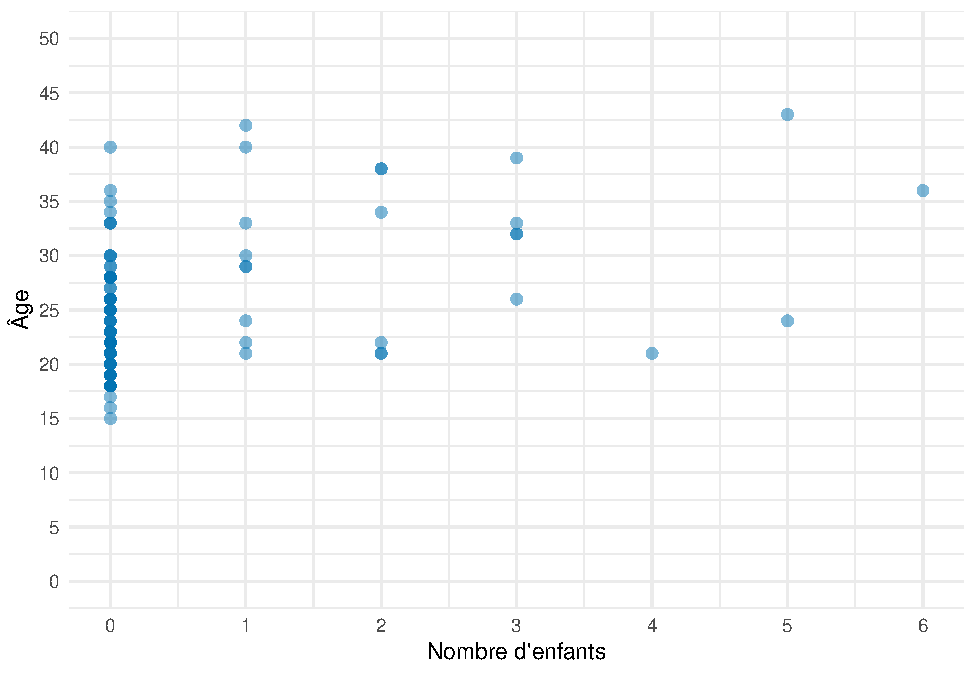
\includegraphics{RMarkdown_files/figure-latex/unnamed-chunk-30-1.pdf}

\begin{itemize}
\tightlist
\item
  Estimation de l'effet de l'appartenance au groupe de traitement sur
  l'intention de migrer:
\end{itemize}

\begin{Shaded}
\begin{Highlighting}[]
\FunctionTok{library}\NormalTok{(nnet)}
\NormalTok{regm }\OtherTok{\textless{}{-}} \FunctionTok{multinom}\NormalTok{(intention }\SpecialCharTok{\textasciitilde{}}\NormalTok{ groupe ,}\AttributeTok{data =}\NormalTok{ copie)}
\end{Highlighting}
\end{Shaded}

\begin{verbatim}
## # weights:  21 (12 variable)
## initial  value 188.753284 
## iter  10 value 116.109117
## iter  20 value 115.901772
## final  value 115.901310 
## converged
\end{verbatim}

\begin{Shaded}
\begin{Highlighting}[]
\NormalTok{tbl }\OtherTok{\textless{}{-}} \FunctionTok{tbl\_regression}\NormalTok{(regm, }\AttributeTok{exponentiate =} \ConstantTok{TRUE}\NormalTok{)}
\NormalTok{tbl}
\end{Highlighting}
\end{Shaded}

\begin{longtable}[]{@{}llccc@{}}
\toprule\noalign{}
\textbf{Outcome} & \textbf{Characteristic} & \textbf{OR} & \textbf{95\%
CI} & \textbf{p-value} \\
\midrule\noalign{}
\endhead
\bottomrule\noalign{}
\endlastfoot
2 & groupe & 0.47 & 0.05, 4.82 & 0.5 \\
3 & groupe & 0.61 & 0.14, 2.58 & 0.5 \\
4 & groupe & 3.56 & 0.64, 19.8 & 0.15 \\
5 & groupe & 1.42 & 0.27, 7.61 & 0.7 \\
6 & groupe & 5.69 & 0.60, 53.9 & 0.13 \\
7 & groupe & 0.00 & 0.00, Inf & \textgreater0.9 \\
\end{longtable}

\begin{Shaded}
\begin{Highlighting}[]
\FunctionTok{library}\NormalTok{(GGally)}
\FunctionTok{ggcoef\_multinom}\NormalTok{(}
\NormalTok{  regm,}
  \AttributeTok{exponentiate =} \ConstantTok{TRUE}\NormalTok{)}
\end{Highlighting}
\end{Shaded}

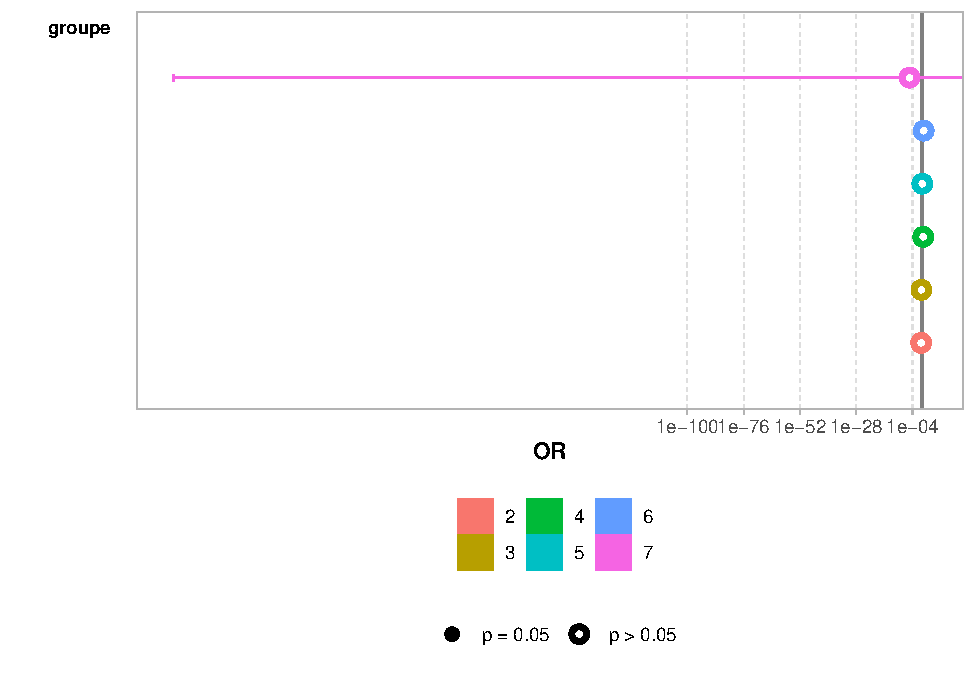
\includegraphics{RMarkdown_files/figure-latex/unnamed-chunk-31-1.pdf}

\begin{Shaded}
\begin{Highlighting}[]
\FunctionTok{library}\NormalTok{(effects)}
\FunctionTok{plot}\NormalTok{(}\FunctionTok{allEffects}\NormalTok{(regm))}
\end{Highlighting}
\end{Shaded}

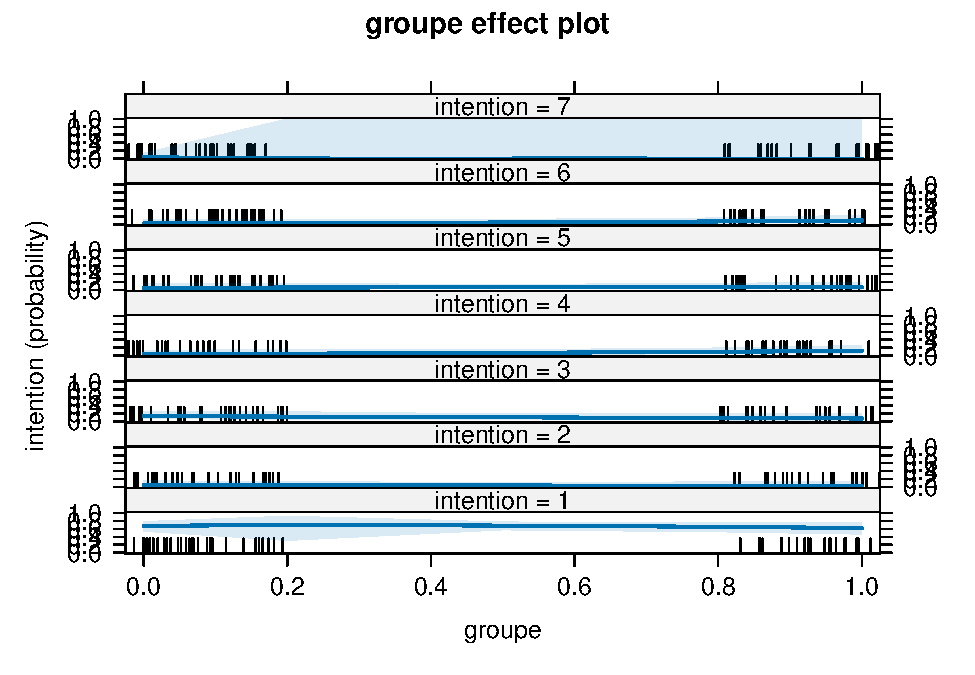
\includegraphics{RMarkdown_files/figure-latex/unnamed-chunk-31-2.pdf}

\begin{itemize}
\tightlist
\item
  Création d'un tableau de régression avec 3 modèles:
\end{itemize}

\begin{Shaded}
\begin{Highlighting}[]
\CommentTok{\# Modèle A : Modèle vide {-} Effet du traitement sur les intentions}
\NormalTok{modele\_A }\OtherTok{\textless{}{-}} \FunctionTok{multinom}\NormalTok{(intention }\SpecialCharTok{\textasciitilde{}}\NormalTok{ groupe, }\AttributeTok{data =}\NormalTok{ copie)}
\end{Highlighting}
\end{Shaded}

\begin{verbatim}
## # weights:  21 (12 variable)
## initial  value 188.753284 
## iter  10 value 116.109117
## iter  20 value 115.901772
## final  value 115.901310 
## converged
\end{verbatim}

\begin{Shaded}
\begin{Highlighting}[]
\NormalTok{tableau\_A }\OtherTok{\textless{}{-}} \FunctionTok{tbl\_regression}\NormalTok{(modele\_A)}

\CommentTok{\# Modèle B : Effet du traitement sur les intentions en tenant compte de l\textquotesingle{}âge et du sexe}
\NormalTok{modele\_B }\OtherTok{\textless{}{-}} \FunctionTok{multinom}\NormalTok{(intention }\SpecialCharTok{\textasciitilde{}}\NormalTok{ groupe }\SpecialCharTok{+}\NormalTok{ age }\SpecialCharTok{+}\NormalTok{ sex, }\AttributeTok{data =}\NormalTok{ copie)}
\end{Highlighting}
\end{Shaded}

\begin{verbatim}
## # weights:  35 (24 variable)
## initial  value 188.753284 
## iter  10 value 114.260695
## iter  20 value 112.317802
## iter  30 value 112.241966
## iter  40 value 112.240901
## final  value 112.240885 
## converged
\end{verbatim}

\begin{Shaded}
\begin{Highlighting}[]
\NormalTok{tableau\_B }\OtherTok{\textless{}{-}} \FunctionTok{tbl\_regression}\NormalTok{(modele\_B)}

\CommentTok{\# Modèle C : Identique au modèle B mais en contrôlant le district}
\NormalTok{modele\_C }\OtherTok{\textless{}{-}} \FunctionTok{multinom}\NormalTok{(intention }\SpecialCharTok{\textasciitilde{}}\NormalTok{ groupe }\SpecialCharTok{+}\NormalTok{ age }\SpecialCharTok{+}\NormalTok{ sex }\SpecialCharTok{+}\NormalTok{ district, }\AttributeTok{data =}\NormalTok{ copie)}
\end{Highlighting}
\end{Shaded}

\begin{verbatim}
## # weights:  42 (30 variable)
## initial  value 188.753284 
## iter  10 value 123.069300
## iter  20 value 110.582195
## iter  30 value 110.364853
## iter  40 value 110.317891
## iter  50 value 110.316861
## final  value 110.316851 
## converged
\end{verbatim}

\begin{Shaded}
\begin{Highlighting}[]
\FunctionTok{ggcoef\_multinom}\NormalTok{(}
\NormalTok{  modele\_C,}
  \AttributeTok{exponentiate =} \ConstantTok{TRUE}\NormalTok{)}
\end{Highlighting}
\end{Shaded}

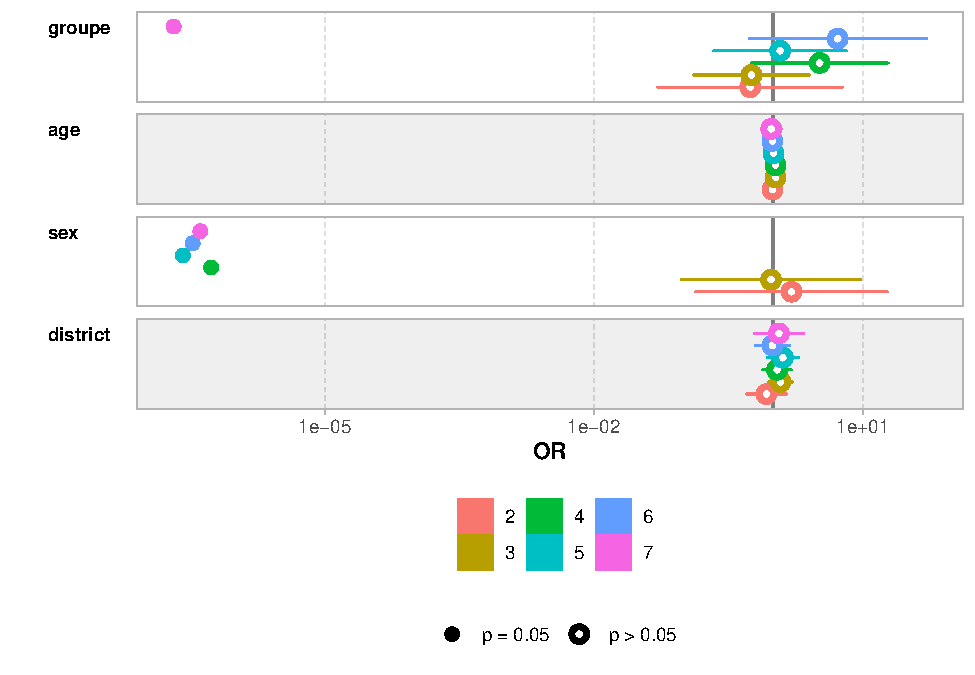
\includegraphics{RMarkdown_files/figure-latex/unnamed-chunk-32-1.pdf}

\begin{Shaded}
\begin{Highlighting}[]
\FunctionTok{plot}\NormalTok{(}\FunctionTok{allEffects}\NormalTok{(modele\_C))}
\end{Highlighting}
\end{Shaded}

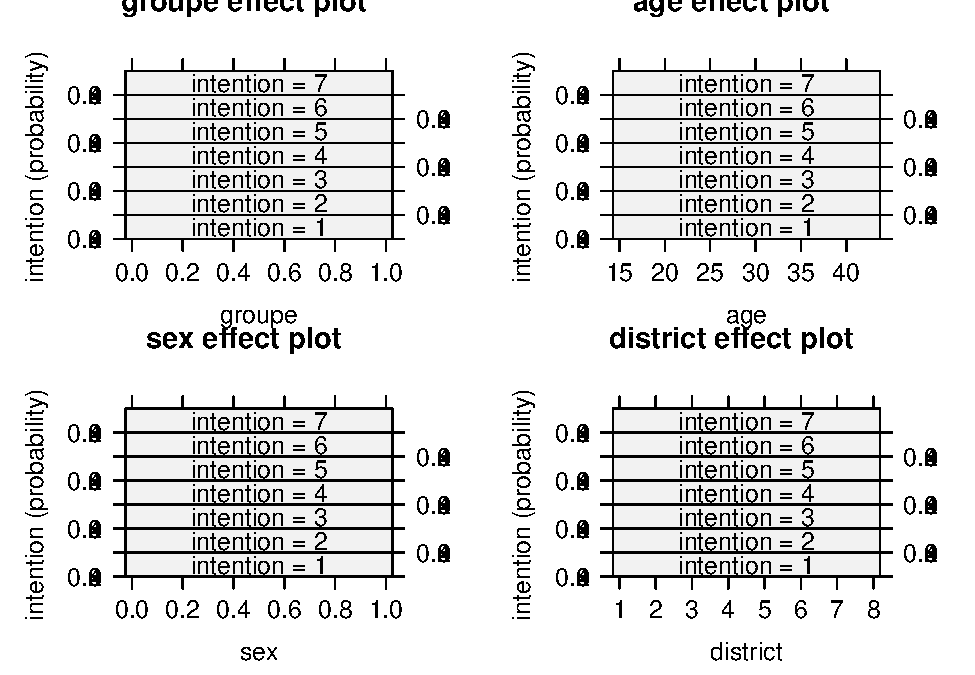
\includegraphics{RMarkdown_files/figure-latex/unnamed-chunk-32-2.pdf}

\begin{Shaded}
\begin{Highlighting}[]
\NormalTok{tableau\_C }\OtherTok{\textless{}{-}} \FunctionTok{tbl\_regression}\NormalTok{(modele\_C)}

\CommentTok{\# Création du tableau récapitulatif des résultats des trois modèles}
\NormalTok{tableau\_final }\OtherTok{\textless{}{-}} \FunctionTok{tbl\_stack}\NormalTok{(}
  \FunctionTok{list}\NormalTok{(tableau\_A, tableau\_B, tableau\_C),}
  \AttributeTok{group\_header =} \FunctionTok{c}\NormalTok{(}\StringTok{"Modèle A"}\NormalTok{,}\StringTok{"Modèle B"}\NormalTok{,}\StringTok{"Modèle C"}\NormalTok{))}\SpecialCharTok{\%\textgreater{}\%}
  \FunctionTok{as\_flex\_table}\NormalTok{()}

\CommentTok{\# Affichage du tableau final}
\NormalTok{tableau\_final}
\end{Highlighting}
\end{Shaded}

\global\setlength{\Oldarrayrulewidth}{\arrayrulewidth}

\global\setlength{\Oldtabcolsep}{\tabcolsep}

\setlength{\tabcolsep}{0pt}

\renewcommand*{\arraystretch}{1.5}



\providecommand{\ascline}[3]{\noalign{\global\arrayrulewidth #1}\arrayrulecolor[HTML]{#2}\cline{#3}}

\begin{longtable}[c]{|p{0.94in}|p{1.30in}|p{0.85in}|p{1.02in}|p{0.82in}}



\ascline{1pt}{000000}{1-5}

\multicolumn{1}{>{\raggedright}m{\dimexpr 0.94in+0\tabcolsep}}{\textcolor[HTML]{000000}{\fontsize{11}{11}\selectfont{\textbf{Group}}}} & \multicolumn{1}{>{\raggedright}m{\dimexpr 1.3in+0\tabcolsep}}{\textcolor[HTML]{000000}{\fontsize{11}{11}\selectfont{\textbf{Characteristic}}}} & \multicolumn{1}{>{\centering}m{\dimexpr 0.85in+0\tabcolsep}}{\textcolor[HTML]{000000}{\fontsize{11}{11}\selectfont{\textbf{log(OR)}}}\textcolor[HTML]{000000}{\textsuperscript{\fontsize{11}{11}\selectfont{1}}}} & \multicolumn{1}{>{\centering}m{\dimexpr 1.02in+0\tabcolsep}}{\textcolor[HTML]{000000}{\fontsize{11}{11}\selectfont{\textbf{95\%\ CI}}}\textcolor[HTML]{000000}{\textsuperscript{\fontsize{11}{11}\selectfont{1}}}} & \multicolumn{1}{>{\centering}m{\dimexpr 0.82in+0\tabcolsep}}{\textcolor[HTML]{000000}{\fontsize{11}{11}\selectfont{\textbf{p-value}}}} \\

\ascline{1pt}{000000}{1-5}\endfirsthead 

\ascline{1pt}{000000}{1-5}

\multicolumn{1}{>{\raggedright}m{\dimexpr 0.94in+0\tabcolsep}}{\textcolor[HTML]{000000}{\fontsize{11}{11}\selectfont{\textbf{Group}}}} & \multicolumn{1}{>{\raggedright}m{\dimexpr 1.3in+0\tabcolsep}}{\textcolor[HTML]{000000}{\fontsize{11}{11}\selectfont{\textbf{Characteristic}}}} & \multicolumn{1}{>{\centering}m{\dimexpr 0.85in+0\tabcolsep}}{\textcolor[HTML]{000000}{\fontsize{11}{11}\selectfont{\textbf{log(OR)}}}\textcolor[HTML]{000000}{\textsuperscript{\fontsize{11}{11}\selectfont{1}}}} & \multicolumn{1}{>{\centering}m{\dimexpr 1.02in+0\tabcolsep}}{\textcolor[HTML]{000000}{\fontsize{11}{11}\selectfont{\textbf{95\%\ CI}}}\textcolor[HTML]{000000}{\textsuperscript{\fontsize{11}{11}\selectfont{1}}}} & \multicolumn{1}{>{\centering}m{\dimexpr 0.82in+0\tabcolsep}}{\textcolor[HTML]{000000}{\fontsize{11}{11}\selectfont{\textbf{p-value}}}} \\

\ascline{1pt}{000000}{1-5}\endhead



\multicolumn{5}{>{\raggedright}m{\dimexpr 4.92in+8\tabcolsep}}{\textcolor[HTML]{000000}{\textsuperscript{\fontsize{11}{11}\selectfont{1}}}\textcolor[HTML]{000000}{\fontsize{11}{11}\selectfont{OR\ =\ Odds\ Ratio,\ CI\ =\ Confidence\ Interval}}} \\

\endfoot



\multicolumn{1}{>{\raggedright}p{\dimexpr 0.94in+0\tabcolsep}}{\textcolor[HTML]{000000}{\fontsize{11}{11}\selectfont{Modèle\ A}}} & \multicolumn{1}{>{\raggedright}p{\dimexpr 1.3in+0\tabcolsep}}{\textcolor[HTML]{000000}{\fontsize{11}{11}\selectfont{groupe}}} & \multicolumn{1}{>{\centering}p{\dimexpr 0.85in+0\tabcolsep}}{\textcolor[HTML]{000000}{\fontsize{11}{11}\selectfont{-0.75}}} & \multicolumn{1}{>{\centering}p{\dimexpr 1.02in+0\tabcolsep}}{\textcolor[HTML]{000000}{\fontsize{11}{11}\selectfont{-3.1,\ 1.6}}} & \multicolumn{1}{>{\centering}p{\dimexpr 0.82in+0\tabcolsep}}{\textcolor[HTML]{000000}{\fontsize{11}{11}\selectfont{0.5}}} \\





\multicolumn{1}{>{\raggedright}p{\dimexpr 0.94in+0\tabcolsep}}{\textcolor[HTML]{000000}{\fontsize{11}{11}\selectfont{}}} & \multicolumn{1}{>{\raggedright}p{\dimexpr 1.3in+0\tabcolsep}}{\textcolor[HTML]{000000}{\fontsize{11}{11}\selectfont{groupe}}} & \multicolumn{1}{>{\centering}p{\dimexpr 0.85in+0\tabcolsep}}{\textcolor[HTML]{000000}{\fontsize{11}{11}\selectfont{-0.49}}} & \multicolumn{1}{>{\centering}p{\dimexpr 1.02in+0\tabcolsep}}{\textcolor[HTML]{000000}{\fontsize{11}{11}\selectfont{-1.9,\ 0.95}}} & \multicolumn{1}{>{\centering}p{\dimexpr 0.82in+0\tabcolsep}}{\textcolor[HTML]{000000}{\fontsize{11}{11}\selectfont{0.5}}} \\





\multicolumn{1}{>{\raggedright}p{\dimexpr 0.94in+0\tabcolsep}}{\textcolor[HTML]{000000}{\fontsize{11}{11}\selectfont{}}} & \multicolumn{1}{>{\raggedright}p{\dimexpr 1.3in+0\tabcolsep}}{\textcolor[HTML]{000000}{\fontsize{11}{11}\selectfont{groupe}}} & \multicolumn{1}{>{\centering}p{\dimexpr 0.85in+0\tabcolsep}}{\textcolor[HTML]{000000}{\fontsize{11}{11}\selectfont{1.3}}} & \multicolumn{1}{>{\centering}p{\dimexpr 1.02in+0\tabcolsep}}{\textcolor[HTML]{000000}{\fontsize{11}{11}\selectfont{-0.45,\ 3.0}}} & \multicolumn{1}{>{\centering}p{\dimexpr 0.82in+0\tabcolsep}}{\textcolor[HTML]{000000}{\fontsize{11}{11}\selectfont{0.15}}} \\





\multicolumn{1}{>{\raggedright}p{\dimexpr 0.94in+0\tabcolsep}}{\textcolor[HTML]{000000}{\fontsize{11}{11}\selectfont{}}} & \multicolumn{1}{>{\raggedright}p{\dimexpr 1.3in+0\tabcolsep}}{\textcolor[HTML]{000000}{\fontsize{11}{11}\selectfont{groupe}}} & \multicolumn{1}{>{\centering}p{\dimexpr 0.85in+0\tabcolsep}}{\textcolor[HTML]{000000}{\fontsize{11}{11}\selectfont{0.35}}} & \multicolumn{1}{>{\centering}p{\dimexpr 1.02in+0\tabcolsep}}{\textcolor[HTML]{000000}{\fontsize{11}{11}\selectfont{-1.3,\ 2.0}}} & \multicolumn{1}{>{\centering}p{\dimexpr 0.82in+0\tabcolsep}}{\textcolor[HTML]{000000}{\fontsize{11}{11}\selectfont{0.7}}} \\





\multicolumn{1}{>{\raggedright}p{\dimexpr 0.94in+0\tabcolsep}}{\textcolor[HTML]{000000}{\fontsize{11}{11}\selectfont{}}} & \multicolumn{1}{>{\raggedright}p{\dimexpr 1.3in+0\tabcolsep}}{\textcolor[HTML]{000000}{\fontsize{11}{11}\selectfont{groupe}}} & \multicolumn{1}{>{\centering}p{\dimexpr 0.85in+0\tabcolsep}}{\textcolor[HTML]{000000}{\fontsize{11}{11}\selectfont{1.7}}} & \multicolumn{1}{>{\centering}p{\dimexpr 1.02in+0\tabcolsep}}{\textcolor[HTML]{000000}{\fontsize{11}{11}\selectfont{-0.51,\ 4.0}}} & \multicolumn{1}{>{\centering}p{\dimexpr 0.82in+0\tabcolsep}}{\textcolor[HTML]{000000}{\fontsize{11}{11}\selectfont{0.13}}} \\





\multicolumn{1}{>{\raggedright}p{\dimexpr 0.94in+0\tabcolsep}}{\textcolor[HTML]{000000}{\fontsize{11}{11}\selectfont{}}} & \multicolumn{1}{>{\raggedright}p{\dimexpr 1.3in+0\tabcolsep}}{\textcolor[HTML]{000000}{\fontsize{11}{11}\selectfont{groupe}}} & \multicolumn{1}{>{\centering}p{\dimexpr 0.85in+0\tabcolsep}}{\textcolor[HTML]{000000}{\fontsize{11}{11}\selectfont{-12}}} & \multicolumn{1}{>{\centering}p{\dimexpr 1.02in+0\tabcolsep}}{\textcolor[HTML]{000000}{\fontsize{11}{11}\selectfont{-734,\ 710}}} & \multicolumn{1}{>{\centering}p{\dimexpr 0.82in+0\tabcolsep}}{\textcolor[HTML]{000000}{\fontsize{11}{11}\selectfont{>0.9}}} \\





\multicolumn{1}{>{\raggedright}p{\dimexpr 0.94in+0\tabcolsep}}{\textcolor[HTML]{000000}{\fontsize{11}{11}\selectfont{Modèle\ B}}} & \multicolumn{1}{>{\raggedright}p{\dimexpr 1.3in+0\tabcolsep}}{\textcolor[HTML]{000000}{\fontsize{11}{11}\selectfont{groupe}}} & \multicolumn{1}{>{\centering}p{\dimexpr 0.85in+0\tabcolsep}}{\textcolor[HTML]{000000}{\fontsize{11}{11}\selectfont{-0.69}}} & \multicolumn{1}{>{\centering}p{\dimexpr 1.02in+0\tabcolsep}}{\textcolor[HTML]{000000}{\fontsize{11}{11}\selectfont{-3.0,\ 1.6}}} & \multicolumn{1}{>{\centering}p{\dimexpr 0.82in+0\tabcolsep}}{\textcolor[HTML]{000000}{\fontsize{11}{11}\selectfont{0.6}}} \\





\multicolumn{1}{>{\raggedright}p{\dimexpr 0.94in+0\tabcolsep}}{\textcolor[HTML]{000000}{\fontsize{11}{11}\selectfont{}}} & \multicolumn{1}{>{\raggedright}p{\dimexpr 1.3in+0\tabcolsep}}{\textcolor[HTML]{000000}{\fontsize{11}{11}\selectfont{age}}} & \multicolumn{1}{>{\centering}p{\dimexpr 0.85in+0\tabcolsep}}{\textcolor[HTML]{000000}{\fontsize{11}{11}\selectfont{0.00}}} & \multicolumn{1}{>{\centering}p{\dimexpr 1.02in+0\tabcolsep}}{\textcolor[HTML]{000000}{\fontsize{11}{11}\selectfont{-0.16,\ 0.17}}} & \multicolumn{1}{>{\centering}p{\dimexpr 0.82in+0\tabcolsep}}{\textcolor[HTML]{000000}{\fontsize{11}{11}\selectfont{>0.9}}} \\





\multicolumn{1}{>{\raggedright}p{\dimexpr 0.94in+0\tabcolsep}}{\textcolor[HTML]{000000}{\fontsize{11}{11}\selectfont{}}} & \multicolumn{1}{>{\raggedright}p{\dimexpr 1.3in+0\tabcolsep}}{\textcolor[HTML]{000000}{\fontsize{11}{11}\selectfont{sex}}} & \multicolumn{1}{>{\centering}p{\dimexpr 0.85in+0\tabcolsep}}{\textcolor[HTML]{000000}{\fontsize{11}{11}\selectfont{0.61}}} & \multicolumn{1}{>{\centering}p{\dimexpr 1.02in+0\tabcolsep}}{\textcolor[HTML]{000000}{\fontsize{11}{11}\selectfont{-1.8,\ 3.1}}} & \multicolumn{1}{>{\centering}p{\dimexpr 0.82in+0\tabcolsep}}{\textcolor[HTML]{000000}{\fontsize{11}{11}\selectfont{0.6}}} \\





\multicolumn{1}{>{\raggedright}p{\dimexpr 0.94in+0\tabcolsep}}{\textcolor[HTML]{000000}{\fontsize{11}{11}\selectfont{}}} & \multicolumn{1}{>{\raggedright}p{\dimexpr 1.3in+0\tabcolsep}}{\textcolor[HTML]{000000}{\fontsize{11}{11}\selectfont{groupe}}} & \multicolumn{1}{>{\centering}p{\dimexpr 0.85in+0\tabcolsep}}{\textcolor[HTML]{000000}{\fontsize{11}{11}\selectfont{-0.47}}} & \multicolumn{1}{>{\centering}p{\dimexpr 1.02in+0\tabcolsep}}{\textcolor[HTML]{000000}{\fontsize{11}{11}\selectfont{-1.9,\ 1.0}}} & \multicolumn{1}{>{\centering}p{\dimexpr 0.82in+0\tabcolsep}}{\textcolor[HTML]{000000}{\fontsize{11}{11}\selectfont{0.5}}} \\





\multicolumn{1}{>{\raggedright}p{\dimexpr 0.94in+0\tabcolsep}}{\textcolor[HTML]{000000}{\fontsize{11}{11}\selectfont{}}} & \multicolumn{1}{>{\raggedright}p{\dimexpr 1.3in+0\tabcolsep}}{\textcolor[HTML]{000000}{\fontsize{11}{11}\selectfont{age}}} & \multicolumn{1}{>{\centering}p{\dimexpr 0.85in+0\tabcolsep}}{\textcolor[HTML]{000000}{\fontsize{11}{11}\selectfont{0.05}}} & \multicolumn{1}{>{\centering}p{\dimexpr 1.02in+0\tabcolsep}}{\textcolor[HTML]{000000}{\fontsize{11}{11}\selectfont{-0.05,\ 0.15}}} & \multicolumn{1}{>{\centering}p{\dimexpr 0.82in+0\tabcolsep}}{\textcolor[HTML]{000000}{\fontsize{11}{11}\selectfont{0.4}}} \\





\multicolumn{1}{>{\raggedright}p{\dimexpr 0.94in+0\tabcolsep}}{\textcolor[HTML]{000000}{\fontsize{11}{11}\selectfont{}}} & \multicolumn{1}{>{\raggedright}p{\dimexpr 1.3in+0\tabcolsep}}{\textcolor[HTML]{000000}{\fontsize{11}{11}\selectfont{sex}}} & \multicolumn{1}{>{\centering}p{\dimexpr 0.85in+0\tabcolsep}}{\textcolor[HTML]{000000}{\fontsize{11}{11}\selectfont{-0.28}}} & \multicolumn{1}{>{\centering}p{\dimexpr 1.02in+0\tabcolsep}}{\textcolor[HTML]{000000}{\fontsize{11}{11}\selectfont{-2.5,\ 2.0}}} & \multicolumn{1}{>{\centering}p{\dimexpr 0.82in+0\tabcolsep}}{\textcolor[HTML]{000000}{\fontsize{11}{11}\selectfont{0.8}}} \\





\multicolumn{1}{>{\raggedright}p{\dimexpr 0.94in+0\tabcolsep}}{\textcolor[HTML]{000000}{\fontsize{11}{11}\selectfont{}}} & \multicolumn{1}{>{\raggedright}p{\dimexpr 1.3in+0\tabcolsep}}{\textcolor[HTML]{000000}{\fontsize{11}{11}\selectfont{groupe}}} & \multicolumn{1}{>{\centering}p{\dimexpr 0.85in+0\tabcolsep}}{\textcolor[HTML]{000000}{\fontsize{11}{11}\selectfont{1.2}}} & \multicolumn{1}{>{\centering}p{\dimexpr 1.02in+0\tabcolsep}}{\textcolor[HTML]{000000}{\fontsize{11}{11}\selectfont{-0.50,\ 3.0}}} & \multicolumn{1}{>{\centering}p{\dimexpr 0.82in+0\tabcolsep}}{\textcolor[HTML]{000000}{\fontsize{11}{11}\selectfont{0.2}}} \\





\multicolumn{1}{>{\raggedright}p{\dimexpr 0.94in+0\tabcolsep}}{\textcolor[HTML]{000000}{\fontsize{11}{11}\selectfont{}}} & \multicolumn{1}{>{\raggedright}p{\dimexpr 1.3in+0\tabcolsep}}{\textcolor[HTML]{000000}{\fontsize{11}{11}\selectfont{age}}} & \multicolumn{1}{>{\centering}p{\dimexpr 0.85in+0\tabcolsep}}{\textcolor[HTML]{000000}{\fontsize{11}{11}\selectfont{0.06}}} & \multicolumn{1}{>{\centering}p{\dimexpr 1.02in+0\tabcolsep}}{\textcolor[HTML]{000000}{\fontsize{11}{11}\selectfont{-0.07,\ 0.18}}} & \multicolumn{1}{>{\centering}p{\dimexpr 0.82in+0\tabcolsep}}{\textcolor[HTML]{000000}{\fontsize{11}{11}\selectfont{0.4}}} \\





\multicolumn{1}{>{\raggedright}p{\dimexpr 0.94in+0\tabcolsep}}{\textcolor[HTML]{000000}{\fontsize{11}{11}\selectfont{}}} & \multicolumn{1}{>{\raggedright}p{\dimexpr 1.3in+0\tabcolsep}}{\textcolor[HTML]{000000}{\fontsize{11}{11}\selectfont{sex}}} & \multicolumn{1}{>{\centering}p{\dimexpr 0.85in+0\tabcolsep}}{\textcolor[HTML]{000000}{\fontsize{11}{11}\selectfont{-14}}} & \multicolumn{1}{>{\centering}p{\dimexpr 1.02in+0\tabcolsep}}{\textcolor[HTML]{000000}{\fontsize{11}{11}\selectfont{-14,\ -14}}} & \multicolumn{1}{>{\centering}p{\dimexpr 0.82in+0\tabcolsep}}{\textcolor[HTML]{000000}{\fontsize{11}{11}\selectfont{<0.001}}} \\





\multicolumn{1}{>{\raggedright}p{\dimexpr 0.94in+0\tabcolsep}}{\textcolor[HTML]{000000}{\fontsize{11}{11}\selectfont{}}} & \multicolumn{1}{>{\raggedright}p{\dimexpr 1.3in+0\tabcolsep}}{\textcolor[HTML]{000000}{\fontsize{11}{11}\selectfont{groupe}}} & \multicolumn{1}{>{\centering}p{\dimexpr 0.85in+0\tabcolsep}}{\textcolor[HTML]{000000}{\fontsize{11}{11}\selectfont{0.27}}} & \multicolumn{1}{>{\centering}p{\dimexpr 1.02in+0\tabcolsep}}{\textcolor[HTML]{000000}{\fontsize{11}{11}\selectfont{-1.4,\ 2.0}}} & \multicolumn{1}{>{\centering}p{\dimexpr 0.82in+0\tabcolsep}}{\textcolor[HTML]{000000}{\fontsize{11}{11}\selectfont{0.8}}} \\





\multicolumn{1}{>{\raggedright}p{\dimexpr 0.94in+0\tabcolsep}}{\textcolor[HTML]{000000}{\fontsize{11}{11}\selectfont{}}} & \multicolumn{1}{>{\raggedright}p{\dimexpr 1.3in+0\tabcolsep}}{\textcolor[HTML]{000000}{\fontsize{11}{11}\selectfont{age}}} & \multicolumn{1}{>{\centering}p{\dimexpr 0.85in+0\tabcolsep}}{\textcolor[HTML]{000000}{\fontsize{11}{11}\selectfont{-0.01}}} & \multicolumn{1}{>{\centering}p{\dimexpr 1.02in+0\tabcolsep}}{\textcolor[HTML]{000000}{\fontsize{11}{11}\selectfont{-0.15,\ 0.13}}} & \multicolumn{1}{>{\centering}p{\dimexpr 0.82in+0\tabcolsep}}{\textcolor[HTML]{000000}{\fontsize{11}{11}\selectfont{0.9}}} \\





\multicolumn{1}{>{\raggedright}p{\dimexpr 0.94in+0\tabcolsep}}{\textcolor[HTML]{000000}{\fontsize{11}{11}\selectfont{}}} & \multicolumn{1}{>{\raggedright}p{\dimexpr 1.3in+0\tabcolsep}}{\textcolor[HTML]{000000}{\fontsize{11}{11}\selectfont{sex}}} & \multicolumn{1}{>{\centering}p{\dimexpr 0.85in+0\tabcolsep}}{\textcolor[HTML]{000000}{\fontsize{11}{11}\selectfont{-16}}} & \multicolumn{1}{>{\centering}p{\dimexpr 1.02in+0\tabcolsep}}{\textcolor[HTML]{000000}{\fontsize{11}{11}\selectfont{-16,\ -16}}} & \multicolumn{1}{>{\centering}p{\dimexpr 0.82in+0\tabcolsep}}{\textcolor[HTML]{000000}{\fontsize{11}{11}\selectfont{<0.001}}} \\





\multicolumn{1}{>{\raggedright}p{\dimexpr 0.94in+0\tabcolsep}}{\textcolor[HTML]{000000}{\fontsize{11}{11}\selectfont{}}} & \multicolumn{1}{>{\raggedright}p{\dimexpr 1.3in+0\tabcolsep}}{\textcolor[HTML]{000000}{\fontsize{11}{11}\selectfont{groupe}}} & \multicolumn{1}{>{\centering}p{\dimexpr 0.85in+0\tabcolsep}}{\textcolor[HTML]{000000}{\fontsize{11}{11}\selectfont{1.7}}} & \multicolumn{1}{>{\centering}p{\dimexpr 1.02in+0\tabcolsep}}{\textcolor[HTML]{000000}{\fontsize{11}{11}\selectfont{-0.60,\ 3.9}}} & \multicolumn{1}{>{\centering}p{\dimexpr 0.82in+0\tabcolsep}}{\textcolor[HTML]{000000}{\fontsize{11}{11}\selectfont{0.2}}} \\





\multicolumn{1}{>{\raggedright}p{\dimexpr 0.94in+0\tabcolsep}}{\textcolor[HTML]{000000}{\fontsize{11}{11}\selectfont{}}} & \multicolumn{1}{>{\raggedright}p{\dimexpr 1.3in+0\tabcolsep}}{\textcolor[HTML]{000000}{\fontsize{11}{11}\selectfont{age}}} & \multicolumn{1}{>{\centering}p{\dimexpr 0.85in+0\tabcolsep}}{\textcolor[HTML]{000000}{\fontsize{11}{11}\selectfont{-0.02}}} & \multicolumn{1}{>{\centering}p{\dimexpr 1.02in+0\tabcolsep}}{\textcolor[HTML]{000000}{\fontsize{11}{11}\selectfont{-0.19,\ 0.15}}} & \multicolumn{1}{>{\centering}p{\dimexpr 0.82in+0\tabcolsep}}{\textcolor[HTML]{000000}{\fontsize{11}{11}\selectfont{0.8}}} \\





\multicolumn{1}{>{\raggedright}p{\dimexpr 0.94in+0\tabcolsep}}{\textcolor[HTML]{000000}{\fontsize{11}{11}\selectfont{}}} & \multicolumn{1}{>{\raggedright}p{\dimexpr 1.3in+0\tabcolsep}}{\textcolor[HTML]{000000}{\fontsize{11}{11}\selectfont{sex}}} & \multicolumn{1}{>{\centering}p{\dimexpr 0.85in+0\tabcolsep}}{\textcolor[HTML]{000000}{\fontsize{11}{11}\selectfont{-14}}} & \multicolumn{1}{>{\centering}p{\dimexpr 1.02in+0\tabcolsep}}{\textcolor[HTML]{000000}{\fontsize{11}{11}\selectfont{-14,\ -14}}} & \multicolumn{1}{>{\centering}p{\dimexpr 0.82in+0\tabcolsep}}{\textcolor[HTML]{000000}{\fontsize{11}{11}\selectfont{<0.001}}} \\





\multicolumn{1}{>{\raggedright}p{\dimexpr 0.94in+0\tabcolsep}}{\textcolor[HTML]{000000}{\fontsize{11}{11}\selectfont{}}} & \multicolumn{1}{>{\raggedright}p{\dimexpr 1.3in+0\tabcolsep}}{\textcolor[HTML]{000000}{\fontsize{11}{11}\selectfont{groupe}}} & \multicolumn{1}{>{\centering}p{\dimexpr 0.85in+0\tabcolsep}}{\textcolor[HTML]{000000}{\fontsize{11}{11}\selectfont{-14}}} & \multicolumn{1}{>{\centering}p{\dimexpr 1.02in+0\tabcolsep}}{\textcolor[HTML]{000000}{\fontsize{11}{11}\selectfont{-14,\ -14}}} & \multicolumn{1}{>{\centering}p{\dimexpr 0.82in+0\tabcolsep}}{\textcolor[HTML]{000000}{\fontsize{11}{11}\selectfont{<0.001}}} \\





\multicolumn{1}{>{\raggedright}p{\dimexpr 0.94in+0\tabcolsep}}{\textcolor[HTML]{000000}{\fontsize{11}{11}\selectfont{}}} & \multicolumn{1}{>{\raggedright}p{\dimexpr 1.3in+0\tabcolsep}}{\textcolor[HTML]{000000}{\fontsize{11}{11}\selectfont{age}}} & \multicolumn{1}{>{\centering}p{\dimexpr 0.85in+0\tabcolsep}}{\textcolor[HTML]{000000}{\fontsize{11}{11}\selectfont{-0.06}}} & \multicolumn{1}{>{\centering}p{\dimexpr 1.02in+0\tabcolsep}}{\textcolor[HTML]{000000}{\fontsize{11}{11}\selectfont{-0.31,\ 0.19}}} & \multicolumn{1}{>{\centering}p{\dimexpr 0.82in+0\tabcolsep}}{\textcolor[HTML]{000000}{\fontsize{11}{11}\selectfont{0.6}}} \\





\multicolumn{1}{>{\raggedright}p{\dimexpr 0.94in+0\tabcolsep}}{\textcolor[HTML]{000000}{\fontsize{11}{11}\selectfont{}}} & \multicolumn{1}{>{\raggedright}p{\dimexpr 1.3in+0\tabcolsep}}{\textcolor[HTML]{000000}{\fontsize{11}{11}\selectfont{sex}}} & \multicolumn{1}{>{\centering}p{\dimexpr 0.85in+0\tabcolsep}}{\textcolor[HTML]{000000}{\fontsize{11}{11}\selectfont{-15}}} & \multicolumn{1}{>{\centering}p{\dimexpr 1.02in+0\tabcolsep}}{\textcolor[HTML]{000000}{\fontsize{11}{11}\selectfont{-15,\ -15}}} & \multicolumn{1}{>{\centering}p{\dimexpr 0.82in+0\tabcolsep}}{\textcolor[HTML]{000000}{\fontsize{11}{11}\selectfont{<0.001}}} \\





\multicolumn{1}{>{\raggedright}p{\dimexpr 0.94in+0\tabcolsep}}{\textcolor[HTML]{000000}{\fontsize{11}{11}\selectfont{Modèle\ C}}} & \multicolumn{1}{>{\raggedright}p{\dimexpr 1.3in+0\tabcolsep}}{\textcolor[HTML]{000000}{\fontsize{11}{11}\selectfont{groupe}}} & \multicolumn{1}{>{\centering}p{\dimexpr 0.85in+0\tabcolsep}}{\textcolor[HTML]{000000}{\fontsize{11}{11}\selectfont{-0.59}}} & \multicolumn{1}{>{\centering}p{\dimexpr 1.02in+0\tabcolsep}}{\textcolor[HTML]{000000}{\fontsize{11}{11}\selectfont{-3.0,\ 1.8}}} & \multicolumn{1}{>{\centering}p{\dimexpr 0.82in+0\tabcolsep}}{\textcolor[HTML]{000000}{\fontsize{11}{11}\selectfont{0.6}}} \\





\multicolumn{1}{>{\raggedright}p{\dimexpr 0.94in+0\tabcolsep}}{\textcolor[HTML]{000000}{\fontsize{11}{11}\selectfont{}}} & \multicolumn{1}{>{\raggedright}p{\dimexpr 1.3in+0\tabcolsep}}{\textcolor[HTML]{000000}{\fontsize{11}{11}\selectfont{age}}} & \multicolumn{1}{>{\centering}p{\dimexpr 0.85in+0\tabcolsep}}{\textcolor[HTML]{000000}{\fontsize{11}{11}\selectfont{-0.02}}} & \multicolumn{1}{>{\centering}p{\dimexpr 1.02in+0\tabcolsep}}{\textcolor[HTML]{000000}{\fontsize{11}{11}\selectfont{-0.19,\ 0.16}}} & \multicolumn{1}{>{\centering}p{\dimexpr 0.82in+0\tabcolsep}}{\textcolor[HTML]{000000}{\fontsize{11}{11}\selectfont{0.9}}} \\





\multicolumn{1}{>{\raggedright}p{\dimexpr 0.94in+0\tabcolsep}}{\textcolor[HTML]{000000}{\fontsize{11}{11}\selectfont{}}} & \multicolumn{1}{>{\raggedright}p{\dimexpr 1.3in+0\tabcolsep}}{\textcolor[HTML]{000000}{\fontsize{11}{11}\selectfont{sex}}} & \multicolumn{1}{>{\centering}p{\dimexpr 0.85in+0\tabcolsep}}{\textcolor[HTML]{000000}{\fontsize{11}{11}\selectfont{0.47}}} & \multicolumn{1}{>{\centering}p{\dimexpr 1.02in+0\tabcolsep}}{\textcolor[HTML]{000000}{\fontsize{11}{11}\selectfont{-2.0,\ 2.9}}} & \multicolumn{1}{>{\centering}p{\dimexpr 0.82in+0\tabcolsep}}{\textcolor[HTML]{000000}{\fontsize{11}{11}\selectfont{0.7}}} \\





\multicolumn{1}{>{\raggedright}p{\dimexpr 0.94in+0\tabcolsep}}{\textcolor[HTML]{000000}{\fontsize{11}{11}\selectfont{}}} & \multicolumn{1}{>{\raggedright}p{\dimexpr 1.3in+0\tabcolsep}}{\textcolor[HTML]{000000}{\fontsize{11}{11}\selectfont{district}}} & \multicolumn{1}{>{\centering}p{\dimexpr 0.85in+0\tabcolsep}}{\textcolor[HTML]{000000}{\fontsize{11}{11}\selectfont{-0.17}}} & \multicolumn{1}{>{\centering}p{\dimexpr 1.02in+0\tabcolsep}}{\textcolor[HTML]{000000}{\fontsize{11}{11}\selectfont{-0.68,\ 0.34}}} & \multicolumn{1}{>{\centering}p{\dimexpr 0.82in+0\tabcolsep}}{\textcolor[HTML]{000000}{\fontsize{11}{11}\selectfont{0.5}}} \\





\multicolumn{1}{>{\raggedright}p{\dimexpr 0.94in+0\tabcolsep}}{\textcolor[HTML]{000000}{\fontsize{11}{11}\selectfont{}}} & \multicolumn{1}{>{\raggedright}p{\dimexpr 1.3in+0\tabcolsep}}{\textcolor[HTML]{000000}{\fontsize{11}{11}\selectfont{groupe}}} & \multicolumn{1}{>{\centering}p{\dimexpr 0.85in+0\tabcolsep}}{\textcolor[HTML]{000000}{\fontsize{11}{11}\selectfont{-0.55}}} & \multicolumn{1}{>{\centering}p{\dimexpr 1.02in+0\tabcolsep}}{\textcolor[HTML]{000000}{\fontsize{11}{11}\selectfont{-2.0,\ 0.92}}} & \multicolumn{1}{>{\centering}p{\dimexpr 0.82in+0\tabcolsep}}{\textcolor[HTML]{000000}{\fontsize{11}{11}\selectfont{0.5}}} \\





\multicolumn{1}{>{\raggedright}p{\dimexpr 0.94in+0\tabcolsep}}{\textcolor[HTML]{000000}{\fontsize{11}{11}\selectfont{}}} & \multicolumn{1}{>{\raggedright}p{\dimexpr 1.3in+0\tabcolsep}}{\textcolor[HTML]{000000}{\fontsize{11}{11}\selectfont{age}}} & \multicolumn{1}{>{\centering}p{\dimexpr 0.85in+0\tabcolsep}}{\textcolor[HTML]{000000}{\fontsize{11}{11}\selectfont{0.06}}} & \multicolumn{1}{>{\centering}p{\dimexpr 1.02in+0\tabcolsep}}{\textcolor[HTML]{000000}{\fontsize{11}{11}\selectfont{-0.04,\ 0.17}}} & \multicolumn{1}{>{\centering}p{\dimexpr 0.82in+0\tabcolsep}}{\textcolor[HTML]{000000}{\fontsize{11}{11}\selectfont{0.2}}} \\





\multicolumn{1}{>{\raggedright}p{\dimexpr 0.94in+0\tabcolsep}}{\textcolor[HTML]{000000}{\fontsize{11}{11}\selectfont{}}} & \multicolumn{1}{>{\raggedright}p{\dimexpr 1.3in+0\tabcolsep}}{\textcolor[HTML]{000000}{\fontsize{11}{11}\selectfont{sex}}} & \multicolumn{1}{>{\centering}p{\dimexpr 0.85in+0\tabcolsep}}{\textcolor[HTML]{000000}{\fontsize{11}{11}\selectfont{-0.05}}} & \multicolumn{1}{>{\centering}p{\dimexpr 1.02in+0\tabcolsep}}{\textcolor[HTML]{000000}{\fontsize{11}{11}\selectfont{-2.3,\ 2.2}}} & \multicolumn{1}{>{\centering}p{\dimexpr 0.82in+0\tabcolsep}}{\textcolor[HTML]{000000}{\fontsize{11}{11}\selectfont{>0.9}}} \\





\multicolumn{1}{>{\raggedright}p{\dimexpr 0.94in+0\tabcolsep}}{\textcolor[HTML]{000000}{\fontsize{11}{11}\selectfont{}}} & \multicolumn{1}{>{\raggedright}p{\dimexpr 1.3in+0\tabcolsep}}{\textcolor[HTML]{000000}{\fontsize{11}{11}\selectfont{district}}} & \multicolumn{1}{>{\centering}p{\dimexpr 0.85in+0\tabcolsep}}{\textcolor[HTML]{000000}{\fontsize{11}{11}\selectfont{0.19}}} & \multicolumn{1}{>{\centering}p{\dimexpr 1.02in+0\tabcolsep}}{\textcolor[HTML]{000000}{\fontsize{11}{11}\selectfont{-0.11,\ 0.49}}} & \multicolumn{1}{>{\centering}p{\dimexpr 0.82in+0\tabcolsep}}{\textcolor[HTML]{000000}{\fontsize{11}{11}\selectfont{0.2}}} \\





\multicolumn{1}{>{\raggedright}p{\dimexpr 0.94in+0\tabcolsep}}{\textcolor[HTML]{000000}{\fontsize{11}{11}\selectfont{}}} & \multicolumn{1}{>{\raggedright}p{\dimexpr 1.3in+0\tabcolsep}}{\textcolor[HTML]{000000}{\fontsize{11}{11}\selectfont{groupe}}} & \multicolumn{1}{>{\centering}p{\dimexpr 0.85in+0\tabcolsep}}{\textcolor[HTML]{000000}{\fontsize{11}{11}\selectfont{1.2}}} & \multicolumn{1}{>{\centering}p{\dimexpr 1.02in+0\tabcolsep}}{\textcolor[HTML]{000000}{\fontsize{11}{11}\selectfont{-0.56,\ 2.9}}} & \multicolumn{1}{>{\centering}p{\dimexpr 0.82in+0\tabcolsep}}{\textcolor[HTML]{000000}{\fontsize{11}{11}\selectfont{0.2}}} \\





\multicolumn{1}{>{\raggedright}p{\dimexpr 0.94in+0\tabcolsep}}{\textcolor[HTML]{000000}{\fontsize{11}{11}\selectfont{}}} & \multicolumn{1}{>{\raggedright}p{\dimexpr 1.3in+0\tabcolsep}}{\textcolor[HTML]{000000}{\fontsize{11}{11}\selectfont{age}}} & \multicolumn{1}{>{\centering}p{\dimexpr 0.85in+0\tabcolsep}}{\textcolor[HTML]{000000}{\fontsize{11}{11}\selectfont{0.06}}} & \multicolumn{1}{>{\centering}p{\dimexpr 1.02in+0\tabcolsep}}{\textcolor[HTML]{000000}{\fontsize{11}{11}\selectfont{-0.06,\ 0.19}}} & \multicolumn{1}{>{\centering}p{\dimexpr 0.82in+0\tabcolsep}}{\textcolor[HTML]{000000}{\fontsize{11}{11}\selectfont{0.3}}} \\





\multicolumn{1}{>{\raggedright}p{\dimexpr 0.94in+0\tabcolsep}}{\textcolor[HTML]{000000}{\fontsize{11}{11}\selectfont{}}} & \multicolumn{1}{>{\raggedright}p{\dimexpr 1.3in+0\tabcolsep}}{\textcolor[HTML]{000000}{\fontsize{11}{11}\selectfont{sex}}} & \multicolumn{1}{>{\centering}p{\dimexpr 0.85in+0\tabcolsep}}{\textcolor[HTML]{000000}{\fontsize{11}{11}\selectfont{-14}}} & \multicolumn{1}{>{\centering}p{\dimexpr 1.02in+0\tabcolsep}}{\textcolor[HTML]{000000}{\fontsize{11}{11}\selectfont{-14,\ -14}}} & \multicolumn{1}{>{\centering}p{\dimexpr 0.82in+0\tabcolsep}}{\textcolor[HTML]{000000}{\fontsize{11}{11}\selectfont{<0.001}}} \\





\multicolumn{1}{>{\raggedright}p{\dimexpr 0.94in+0\tabcolsep}}{\textcolor[HTML]{000000}{\fontsize{11}{11}\selectfont{}}} & \multicolumn{1}{>{\raggedright}p{\dimexpr 1.3in+0\tabcolsep}}{\textcolor[HTML]{000000}{\fontsize{11}{11}\selectfont{district}}} & \multicolumn{1}{>{\centering}p{\dimexpr 0.85in+0\tabcolsep}}{\textcolor[HTML]{000000}{\fontsize{11}{11}\selectfont{0.10}}} & \multicolumn{1}{>{\centering}p{\dimexpr 1.02in+0\tabcolsep}}{\textcolor[HTML]{000000}{\fontsize{11}{11}\selectfont{-0.27,\ 0.47}}} & \multicolumn{1}{>{\centering}p{\dimexpr 0.82in+0\tabcolsep}}{\textcolor[HTML]{000000}{\fontsize{11}{11}\selectfont{0.6}}} \\





\multicolumn{1}{>{\raggedright}p{\dimexpr 0.94in+0\tabcolsep}}{\textcolor[HTML]{000000}{\fontsize{11}{11}\selectfont{}}} & \multicolumn{1}{>{\raggedright}p{\dimexpr 1.3in+0\tabcolsep}}{\textcolor[HTML]{000000}{\fontsize{11}{11}\selectfont{groupe}}} & \multicolumn{1}{>{\centering}p{\dimexpr 0.85in+0\tabcolsep}}{\textcolor[HTML]{000000}{\fontsize{11}{11}\selectfont{0.18}}} & \multicolumn{1}{>{\centering}p{\dimexpr 1.02in+0\tabcolsep}}{\textcolor[HTML]{000000}{\fontsize{11}{11}\selectfont{-1.5,\ 1.9}}} & \multicolumn{1}{>{\centering}p{\dimexpr 0.82in+0\tabcolsep}}{\textcolor[HTML]{000000}{\fontsize{11}{11}\selectfont{0.8}}} \\





\multicolumn{1}{>{\raggedright}p{\dimexpr 0.94in+0\tabcolsep}}{\textcolor[HTML]{000000}{\fontsize{11}{11}\selectfont{}}} & \multicolumn{1}{>{\raggedright}p{\dimexpr 1.3in+0\tabcolsep}}{\textcolor[HTML]{000000}{\fontsize{11}{11}\selectfont{age}}} & \multicolumn{1}{>{\centering}p{\dimexpr 0.85in+0\tabcolsep}}{\textcolor[HTML]{000000}{\fontsize{11}{11}\selectfont{0.01}}} & \multicolumn{1}{>{\centering}p{\dimexpr 1.02in+0\tabcolsep}}{\textcolor[HTML]{000000}{\fontsize{11}{11}\selectfont{-0.13,\ 0.15}}} & \multicolumn{1}{>{\centering}p{\dimexpr 0.82in+0\tabcolsep}}{\textcolor[HTML]{000000}{\fontsize{11}{11}\selectfont{0.9}}} \\





\multicolumn{1}{>{\raggedright}p{\dimexpr 0.94in+0\tabcolsep}}{\textcolor[HTML]{000000}{\fontsize{11}{11}\selectfont{}}} & \multicolumn{1}{>{\raggedright}p{\dimexpr 1.3in+0\tabcolsep}}{\textcolor[HTML]{000000}{\fontsize{11}{11}\selectfont{sex}}} & \multicolumn{1}{>{\centering}p{\dimexpr 0.85in+0\tabcolsep}}{\textcolor[HTML]{000000}{\fontsize{11}{11}\selectfont{-15}}} & \multicolumn{1}{>{\centering}p{\dimexpr 1.02in+0\tabcolsep}}{\textcolor[HTML]{000000}{\fontsize{11}{11}\selectfont{-15,\ -15}}} & \multicolumn{1}{>{\centering}p{\dimexpr 0.82in+0\tabcolsep}}{\textcolor[HTML]{000000}{\fontsize{11}{11}\selectfont{<0.001}}} \\





\multicolumn{1}{>{\raggedright}p{\dimexpr 0.94in+0\tabcolsep}}{\textcolor[HTML]{000000}{\fontsize{11}{11}\selectfont{}}} & \multicolumn{1}{>{\raggedright}p{\dimexpr 1.3in+0\tabcolsep}}{\textcolor[HTML]{000000}{\fontsize{11}{11}\selectfont{district}}} & \multicolumn{1}{>{\centering}p{\dimexpr 0.85in+0\tabcolsep}}{\textcolor[HTML]{000000}{\fontsize{11}{11}\selectfont{0.25}}} & \multicolumn{1}{>{\centering}p{\dimexpr 1.02in+0\tabcolsep}}{\textcolor[HTML]{000000}{\fontsize{11}{11}\selectfont{-0.15,\ 0.65}}} & \multicolumn{1}{>{\centering}p{\dimexpr 0.82in+0\tabcolsep}}{\textcolor[HTML]{000000}{\fontsize{11}{11}\selectfont{0.2}}} \\





\multicolumn{1}{>{\raggedright}p{\dimexpr 0.94in+0\tabcolsep}}{\textcolor[HTML]{000000}{\fontsize{11}{11}\selectfont{}}} & \multicolumn{1}{>{\raggedright}p{\dimexpr 1.3in+0\tabcolsep}}{\textcolor[HTML]{000000}{\fontsize{11}{11}\selectfont{groupe}}} & \multicolumn{1}{>{\centering}p{\dimexpr 0.85in+0\tabcolsep}}{\textcolor[HTML]{000000}{\fontsize{11}{11}\selectfont{1.7}}} & \multicolumn{1}{>{\centering}p{\dimexpr 1.02in+0\tabcolsep}}{\textcolor[HTML]{000000}{\fontsize{11}{11}\selectfont{-0.61,\ 3.9}}} & \multicolumn{1}{>{\centering}p{\dimexpr 0.82in+0\tabcolsep}}{\textcolor[HTML]{000000}{\fontsize{11}{11}\selectfont{0.2}}} \\





\multicolumn{1}{>{\raggedright}p{\dimexpr 0.94in+0\tabcolsep}}{\textcolor[HTML]{000000}{\fontsize{11}{11}\selectfont{}}} & \multicolumn{1}{>{\raggedright}p{\dimexpr 1.3in+0\tabcolsep}}{\textcolor[HTML]{000000}{\fontsize{11}{11}\selectfont{age}}} & \multicolumn{1}{>{\centering}p{\dimexpr 0.85in+0\tabcolsep}}{\textcolor[HTML]{000000}{\fontsize{11}{11}\selectfont{-0.02}}} & \multicolumn{1}{>{\centering}p{\dimexpr 1.02in+0\tabcolsep}}{\textcolor[HTML]{000000}{\fontsize{11}{11}\selectfont{-0.19,\ 0.15}}} & \multicolumn{1}{>{\centering}p{\dimexpr 0.82in+0\tabcolsep}}{\textcolor[HTML]{000000}{\fontsize{11}{11}\selectfont{0.8}}} \\





\multicolumn{1}{>{\raggedright}p{\dimexpr 0.94in+0\tabcolsep}}{\textcolor[HTML]{000000}{\fontsize{11}{11}\selectfont{}}} & \multicolumn{1}{>{\raggedright}p{\dimexpr 1.3in+0\tabcolsep}}{\textcolor[HTML]{000000}{\fontsize{11}{11}\selectfont{sex}}} & \multicolumn{1}{>{\centering}p{\dimexpr 0.85in+0\tabcolsep}}{\textcolor[HTML]{000000}{\fontsize{11}{11}\selectfont{-15}}} & \multicolumn{1}{>{\centering}p{\dimexpr 1.02in+0\tabcolsep}}{\textcolor[HTML]{000000}{\fontsize{11}{11}\selectfont{-15,\ -15}}} & \multicolumn{1}{>{\centering}p{\dimexpr 0.82in+0\tabcolsep}}{\textcolor[HTML]{000000}{\fontsize{11}{11}\selectfont{<0.001}}} \\





\multicolumn{1}{>{\raggedright}p{\dimexpr 0.94in+0\tabcolsep}}{\textcolor[HTML]{000000}{\fontsize{11}{11}\selectfont{}}} & \multicolumn{1}{>{\raggedright}p{\dimexpr 1.3in+0\tabcolsep}}{\textcolor[HTML]{000000}{\fontsize{11}{11}\selectfont{district}}} & \multicolumn{1}{>{\centering}p{\dimexpr 0.85in+0\tabcolsep}}{\textcolor[HTML]{000000}{\fontsize{11}{11}\selectfont{-0.02}}} & \multicolumn{1}{>{\centering}p{\dimexpr 1.02in+0\tabcolsep}}{\textcolor[HTML]{000000}{\fontsize{11}{11}\selectfont{-0.45,\ 0.42}}} & \multicolumn{1}{>{\centering}p{\dimexpr 0.82in+0\tabcolsep}}{\textcolor[HTML]{000000}{\fontsize{11}{11}\selectfont{>0.9}}} \\





\multicolumn{1}{>{\raggedright}p{\dimexpr 0.94in+0\tabcolsep}}{\textcolor[HTML]{000000}{\fontsize{11}{11}\selectfont{}}} & \multicolumn{1}{>{\raggedright}p{\dimexpr 1.3in+0\tabcolsep}}{\textcolor[HTML]{000000}{\fontsize{11}{11}\selectfont{groupe}}} & \multicolumn{1}{>{\centering}p{\dimexpr 0.85in+0\tabcolsep}}{\textcolor[HTML]{000000}{\fontsize{11}{11}\selectfont{-15}}} & \multicolumn{1}{>{\centering}p{\dimexpr 1.02in+0\tabcolsep}}{\textcolor[HTML]{000000}{\fontsize{11}{11}\selectfont{-15,\ -15}}} & \multicolumn{1}{>{\centering}p{\dimexpr 0.82in+0\tabcolsep}}{\textcolor[HTML]{000000}{\fontsize{11}{11}\selectfont{<0.001}}} \\





\multicolumn{1}{>{\raggedright}p{\dimexpr 0.94in+0\tabcolsep}}{\textcolor[HTML]{000000}{\fontsize{11}{11}\selectfont{}}} & \multicolumn{1}{>{\raggedright}p{\dimexpr 1.3in+0\tabcolsep}}{\textcolor[HTML]{000000}{\fontsize{11}{11}\selectfont{age}}} & \multicolumn{1}{>{\centering}p{\dimexpr 0.85in+0\tabcolsep}}{\textcolor[HTML]{000000}{\fontsize{11}{11}\selectfont{-0.05}}} & \multicolumn{1}{>{\centering}p{\dimexpr 1.02in+0\tabcolsep}}{\textcolor[HTML]{000000}{\fontsize{11}{11}\selectfont{-0.30,\ 0.20}}} & \multicolumn{1}{>{\centering}p{\dimexpr 0.82in+0\tabcolsep}}{\textcolor[HTML]{000000}{\fontsize{11}{11}\selectfont{0.7}}} \\





\multicolumn{1}{>{\raggedright}p{\dimexpr 0.94in+0\tabcolsep}}{\textcolor[HTML]{000000}{\fontsize{11}{11}\selectfont{}}} & \multicolumn{1}{>{\raggedright}p{\dimexpr 1.3in+0\tabcolsep}}{\textcolor[HTML]{000000}{\fontsize{11}{11}\selectfont{sex}}} & \multicolumn{1}{>{\centering}p{\dimexpr 0.85in+0\tabcolsep}}{\textcolor[HTML]{000000}{\fontsize{11}{11}\selectfont{-15}}} & \multicolumn{1}{>{\centering}p{\dimexpr 1.02in+0\tabcolsep}}{\textcolor[HTML]{000000}{\fontsize{11}{11}\selectfont{-15,\ -15}}} & \multicolumn{1}{>{\centering}p{\dimexpr 0.82in+0\tabcolsep}}{\textcolor[HTML]{000000}{\fontsize{11}{11}\selectfont{<0.001}}} \\





\multicolumn{1}{>{\raggedright}p{\dimexpr 0.94in+0\tabcolsep}}{\textcolor[HTML]{000000}{\fontsize{11}{11}\selectfont{}}} & \multicolumn{1}{>{\raggedright}p{\dimexpr 1.3in+0\tabcolsep}}{\textcolor[HTML]{000000}{\fontsize{11}{11}\selectfont{district}}} & \multicolumn{1}{>{\centering}p{\dimexpr 0.85in+0\tabcolsep}}{\textcolor[HTML]{000000}{\fontsize{11}{11}\selectfont{0.15}}} & \multicolumn{1}{>{\centering}p{\dimexpr 1.02in+0\tabcolsep}}{\textcolor[HTML]{000000}{\fontsize{11}{11}\selectfont{-0.48,\ 0.78}}} & \multicolumn{1}{>{\centering}p{\dimexpr 0.82in+0\tabcolsep}}{\textcolor[HTML]{000000}{\fontsize{11}{11}\selectfont{0.6}}} \\

\ascline{1pt}{000000}{1-5}



\end{longtable}



\arrayrulecolor[HTML]{000000}

\global\setlength{\arrayrulewidth}{\Oldarrayrulewidth}

\global\setlength{\tabcolsep}{\Oldtabcolsep}

\renewcommand*{\arraystretch}{1}

\hypertarget{partie-3}{%
\section{Partie 3:}\label{partie-3}}

\end{document}
